\documentclass[12pt,a4paper]{article}
\usepackage{ifthen} 
\newboolean{pdflatex}
\setboolean{pdflatex}{true} 
\newboolean{articletitles}
\setboolean{articletitles}{true}
\newboolean{uprightparticles}
\setboolean{uprightparticles}{false}
\def\paperauthors{LHCb Collaboration}
\def\paperasciititle{Multiplicity Dependence of ratio of production of psi(2S) over J/psi in pp collisions at center of mass energy 13 TeV} 
\def\papertitle{Multiplicity dependence of $\sigma_{\psitwos}/\sigma_{\jpsi}$ in $pp$ collisions at $\sqrt{s}=13$ TeV} 
\def\paperkeywords{{High Energy Physics}, {LHCb}} 
\def\papercopyright{\the\year\ CERN for the benefit of the LHCb collaboration} 
\def\paperlicence{CC BY 4.0 licence}
\def\paperlicenceurl{https://creativecommons.org/licenses/by/4.0/}
%%%%%%%%%%%%%%%%%%%%%%%%%%%%%%%%%%%%%%%%%%%%%%%%%%%%%%%%%%%%%%%%%%%%%%
%                                                                    %
% !!!!!!!!!!!!!!!!!!! DO NOT EDIT THIS FILE !!!!!!!!!!!!!!!!!!!!!!!! %
%                                                                    %
% THE EB MAY OVERWRITE IT TO REFLECT LATEST CHANGES IN THE TEMPLATE  %
%                                                                    %
% You may define your own macros and packages in main.tex or add     %
% additional local files                                             %
%%%%%%%%%%%%%%%%%%%%%%%%%%%%%%%%%%%%%%%%%%%%%%%%%%%%%%%%%%%%%%%%%%%%%%
% THis file contains all the default packages and modifications for
% LHCb formatting

%% %%%%%%%%%%%%%%%%%%
%%  Page formatting
%% %%%%%%%%%%%%%%%%%%
%%\usepackage[margin=1in]{geometry}
\usepackage[top=1in, bottom=1.25in, left=1in, right=1in]{geometry}

% fallback for manual settings... uncomment if the geometry package is not available
%
%\voffset=-11mm
%\textheight=220mm
%\textwidth=160mm
%\oddsidemargin=0mm
%\evensidemargin=0mm

\columnsep=5mm
\addtolength{\belowcaptionskip}{0.5em}

\renewcommand{\textfraction}{0.01}
\renewcommand{\floatpagefraction}{0.8} % changed from 0.99
\renewcommand{\topfraction}{0.9}
\renewcommand{\bottomfraction}{0.9}

% Allow the page size to vary a bit ...
\raggedbottom
% To avoid Latex to be too fussy with line breaking ...
\sloppy

%% %%%%%%%%%%%%%%%%%%%%%%%
%% Packages to be used
%% %%%%%%%%%%%%%%%%%%%%%%% 
\usepackage{microtype}
\usepackage{lineno}  % for line numbering during review
\usepackage{xspace} % To avoid problems with missing or double spaces after
                    % predefined symbold
\usepackage{caption} %these three command get the figure and table captions automatically small
\renewcommand{\captionfont}{\small}
\renewcommand{\captionlabelfont}{\small}

%% Graphics
\usepackage{graphicx}  % to include figures (can also use other packages)
\usepackage{color}
\usepackage{colortbl}
\graphicspath{{./figs/}} % Make Latex search fig subdir for figures
% \DeclareGraphicsExtensions{.pdf,.PDF,.png,.PNG}   % not needed

%% Math
\usepackage{amsmath} % Adds a large collection of math symbols
\usepackage{amssymb}
\usepackage{amsfonts}
\usepackage{upgreek} % Adds in support for greek letters in roman typeset

%% fix to allow peaceful coexistence of line numbering and
%% mathematical objects
%% http://www.latex-community.org/forum/viewtopic.php?f=5&t=163
%%
\newcommand*\patchAmsMathEnvironmentForLineno[1]{%
\expandafter\let\csname old#1\expandafter\endcsname\csname #1\endcsname
\expandafter\let\csname oldend#1\expandafter\endcsname\csname
end#1\endcsname
 \renewenvironment{#1}%
   {\linenomath\csname old#1\endcsname}%
   {\csname oldend#1\endcsname\endlinenomath}%
}
\newcommand*\patchBothAmsMathEnvironmentsForLineno[1]{%
  \patchAmsMathEnvironmentForLineno{#1}%
  \patchAmsMathEnvironmentForLineno{#1*}%
}
\AtBeginDocument{%
\patchBothAmsMathEnvironmentsForLineno{equation}%
\patchBothAmsMathEnvironmentsForLineno{align}%
\patchBothAmsMathEnvironmentsForLineno{flalign}%
\patchBothAmsMathEnvironmentsForLineno{alignat}%
\patchBothAmsMathEnvironmentsForLineno{gather}%
\patchBothAmsMathEnvironmentsForLineno{multline}%
\patchBothAmsMathEnvironmentsForLineno{eqnarray}%
}

% Get hyperlinks to captions and in references.
% These do not work with revtex. Use "hypertext" as class option instead.

\usepackage{hyperxmp}

\usepackage[pdftex,
            pdfauthor={\paperauthors},
            pdftitle={\paperasciititle},
            pdfkeywords={\paperkeywords},
            pdfcopyright={Copyright (C) \papercopyright},
            pdflicenseurl={\paperlicenceurl}]{hyperref}
% if you have a mysterious compilation error at this line, check there are only ascii characters in \paperasciititle (main.tex)

% overleaf comments
\usepackage[colorinlistoftodos,textsize=scriptsize]{todonotes}

% get footnotes below floats
\usepackage[bottom,flushmargin,hang,multiple]{footmisc}

\usepackage[all]{hypcap} % Internal hyperlinks to floats.

%%%%%%%%%%%%%%%%%%%%%%%%%%%%%%%%%%%%%%%%%%%%%%%%%%%%%%%%%%%%%%%%%%%%%%%%
%%%                                                                    %
%%% !!!!!!!!!!!!!!!!!!! DO NOT EDIT THIS FILE !!!!!!!!!!!!!!!!!!!!!!!! %
%%%                                                                    %
%%% THE EB MAY OVERWRITE IT TO REFLECT LATEST CHANGES IN THE TEMPLATE  %
%%%                                                                    %
%%% You may define your own macros and packages in main.tex or add     %
%%% additional local files                                             %
%%%%%%%%%%%%%%%%%%%%%%%%%%%%%%%%%%%%%%%%%%%%%%%%%%%%%%%%%%%%%%%%%%%%%%%%
%%% ======================================================================
%%% Purpose: Standard LHCb aliases
%%% Author: Originally Ulrik Egede, adapted by Tomasz Skwarnicki for templates,
%%% rewritten by Chris Parkes
%%% Maintainer : Ulrik Egede (2010 - 2012)
%%% Maintainer : Rolf Oldeman (2012 - 2014)
%%% Maintainer : Patrick Koppenburg (2018--2020)
%%% =======================================================================
%%% To use this file outside the normal LHCb document environment, the
%%% following should be added in a preamble (before \begin{document}
%%%
%%%\usepackage{ifthen} 
%%%\newboolean{uprightparticles}
%%%\setboolean{uprightparticles}{false} %Set true for upright particle symbols
\usepackage{xspace} 
\usepackage{upgreek}


%%%%%%%%%%%%%%%%%%%%%%%%%%%%%%%%%%%%%%%%%%%%%%%%%%%%%%%%%%%%
%%%
%%% The following is to ensure that the template automatically can process
%%% this file.
%%%
%%% Add comments with at least three %%% preceding.
%%% Add new sections with one % preceding
%%% Add new subsections with two %% preceding
%%%
%%% For upper greek letters, Xires and Xiresbar will be the particles without the charge
%%% States with charge are called Xiz and Xim  
%%%
%%%%%%%%%%%%%%%%%%%%%%%%%%%%%%%%%%%%%%%%%%%%%%%%%%%%%%%%%%%%

%%%%%%%%%%%%%
% Experiments
%%%%%%%%%%%%%
\def\lhcb   {\mbox{LHCb}\xspace}
\def\atlas  {\mbox{ATLAS}\xspace}
\def\cms    {\mbox{CMS}\xspace}
\def\alice  {\mbox{ALICE}\xspace}
\def\babar  {\mbox{BaBar}\xspace}
\def\belle  {\mbox{Belle}\xspace}
\def\belletwo {\mbox{Belle~II}\xspace}
\def\besiii {\mbox{BESIII}\xspace}
\def\cleo   {\mbox{CLEO}\xspace}
\def\cdf    {\mbox{CDF}\xspace}
\def\dzero  {\mbox{D0}\xspace}
\def\aleph  {\mbox{ALEPH}\xspace}
\def\delphi {\mbox{DELPHI}\xspace}
\def\opal   {\mbox{OPAL}\xspace}
\def\lthree {\mbox{L3}\xspace}
\def\sld    {\mbox{SLD}\xspace}
%%%\def\argus  {\mbox{ARGUS}\xspace}
%%%\def\uaone  {\mbox{UA1}\xspace}
%%%\def\uatwo  {\mbox{UA2}\xspace}
%%%\def\ux85 {\mbox{UX85}\xspace}
\def\cern {\mbox{CERN}\xspace}
\def\lhc    {\mbox{LHC}\xspace}
\def\lep    {\mbox{LEP}\xspace}
\def\tevatron {Tevatron\xspace}
\def\bfactories {\mbox{\B Factories}\xspace}
\def\bfactory   {\mbox{\B Factory}\xspace}
\def\upgradeone {\mbox{Upgrade~I}\xspace}
\def\upgradetwo {\mbox{Upgrade~II}\xspace}

%% LHCb sub-detectors and sub-systems

%%%\def\pu     {PU\xspace}
\def\velo   {VELO\xspace}
\def\rich   {RICH\xspace}
\def\richone {RICH1\xspace}
\def\richtwo {RICH2\xspace}
\def\ttracker {TT\xspace}
\def\intr   {IT\xspace}
\def\st     {ST\xspace}
\def\ot     {OT\xspace}
\def\herschel {\mbox{\textsc{HeRSCheL}}\xspace}
%%%\def\Tone   {T1\xspace}
%%%\def\Ttwo   {T2\xspace}
%%%\def\Tthree {T3\xspace}
%%%\def\Mone   {M1\xspace}
%%%\def\Mtwo   {M2\xspace}
%%%\def\Mthree {M3\xspace}
%%%\def\Mfour  {M4\xspace}
%%%\def\Mfive  {M5\xspace}
\def\spd    {SPD\xspace}
\def\presh  {PS\xspace}
\def\ecal   {ECAL\xspace}
\def\hcal   {HCAL\xspace}
%%%\def\bcm    {BCM\xspace}
\def\MagUp {\mbox{\em Mag\kern -0.05em Up}\xspace}
\def\MagDown {\mbox{\em MagDown}\xspace}

\def\ode    {ODE\xspace}
\def\daq    {DAQ\xspace}
\def\tfc    {TFC\xspace}
\def\ecs    {ECS\xspace}
\def\lone   {L0\xspace}
\def\hlt    {HLT\xspace}
\def\hltone {HLT1\xspace}
\def\hlttwo {HLT2\xspace}

%%% Upright (not slanted) Particles

\ifthenelse{\boolean{uprightparticles}}%
{\def\Palpha      {\ensuremath{\upalpha}\xspace}
 \def\Pbeta       {\ensuremath{\upbeta}\xspace}
 \def\Pgamma      {\ensuremath{\upgamma}\xspace}                 
 \def\Pdelta      {\ensuremath{\updelta}\xspace}                 
 \def\Pepsilon    {\ensuremath{\upepsilon}\xspace}                 
 \def\Pvarepsilon {\ensuremath{\upvarepsilon}\xspace}                 
 \def\Pzeta       {\ensuremath{\upzeta}\xspace}                 
 \def\Peta        {\ensuremath{\upeta}\xspace}
 \def\Ptheta      {\ensuremath{\uptheta}\xspace}                 
 \def\Pvartheta   {\ensuremath{\upvartheta}\xspace}                 
 \def\Piota       {\ensuremath{\upiota}\xspace}                 
 \def\Pkappa      {\ensuremath{\upkappa}\xspace}                 
 \def\Plambda     {\ensuremath{\uplambda}\xspace}                 
 \def\Pmu         {\ensuremath{\upmu}\xspace}                 
 \def\Pnu         {\ensuremath{\upnu}\xspace}                 
 \def\Pxi         {\ensuremath{\upxi}\xspace}                 
 \def\Ppi         {\ensuremath{\uppi}\xspace}                 
 \def\Pvarpi      {\ensuremath{\upvarpi}\xspace}                 
 \def\Prho        {\ensuremath{\uprho}\xspace}                 
 \def\Pvarrho     {\ensuremath{\upvarrho}\xspace}                 
 \def\Ptau        {\ensuremath{\uptau}\xspace}                 
 \def\Pupsilon    {\ensuremath{\upupsilon}\xspace}                 
 \def\Pphi        {\ensuremath{\upphi}\xspace}                 
 \def\Pvarphi     {\ensuremath{\upvarphi}\xspace}                 
 \def\Pchi        {\ensuremath{\upchi}\xspace}                 
 \def\Ppsi        {\ensuremath{\uppsi}\xspace}                 
 \def\Pomega      {\ensuremath{\upomega}\xspace}                 

 \def\PDelta      {\ensuremath{\Delta}\xspace}                 
 \def\PXi         {\ensuremath{\Xi}\xspace}                 
 \def\PLambda     {\ensuremath{\Lambda}\xspace}                 
 \def\PSigma      {\ensuremath{\Sigma}\xspace}                 
 \def\POmega      {\ensuremath{\Omega}\xspace}                 
 \def\PUpsilon    {\ensuremath{\Upsilon}\xspace}
 \let\oldPi\Pi
 \def\PPi         {\ensuremath{\oldPi}\xspace}                 
               

 \def\PA      {\ensuremath{\mathrm{A}}\xspace}                 
 \def\PB      {\ensuremath{\mathrm{B}}\xspace}                 
 \def\PC      {\ensuremath{\mathrm{C}}\xspace}                 
 \def\PD      {\ensuremath{\mathrm{D}}\xspace}                 
 \def\PE      {\ensuremath{\mathrm{E}}\xspace}                 
 \def\PF      {\ensuremath{\mathrm{F}}\xspace}                 
 \def\PG      {\ensuremath{\mathrm{G}}\xspace}                 
 \def\PH      {\ensuremath{\mathrm{H}}\xspace}                 
 \def\PI      {\ensuremath{\mathrm{I}}\xspace}                 
 \def\PJ      {\ensuremath{\mathrm{J}}\xspace}                 
 \def\PK      {\ensuremath{\mathrm{K}}\xspace}                 
 \def\PL      {\ensuremath{\mathrm{L}}\xspace}                 
 \def\PM      {\ensuremath{\mathrm{M}}\xspace}                 
 \def\PN      {\ensuremath{\mathrm{N}}\xspace}                 
 \def\PO      {\ensuremath{\mathrm{O}}\xspace}                 
 \def\PP      {\ensuremath{\mathrm{P}}\xspace}                 
 \def\PQ      {\ensuremath{\mathrm{Q}}\xspace}                 
 \def\PR      {\ensuremath{\mathrm{R}}\xspace}                 
 \def\PS      {\ensuremath{\mathrm{S}}\xspace}                 
 \def\PT      {\ensuremath{\mathrm{T}}\xspace}                 
 \def\PU      {\ensuremath{\mathrm{U}}\xspace}                 
 \def\PV      {\ensuremath{\mathrm{V}}\xspace}                 
 \def\PW      {\ensuremath{\mathrm{W}}\xspace}                 
 \def\PX      {\ensuremath{\mathrm{X}}\xspace}                 
 \def\PY      {\ensuremath{\mathrm{Y}}\xspace}                 
 \def\PZ      {\ensuremath{\mathrm{Z}}\xspace}                 
 \def\Pa      {\ensuremath{\mathrm{a}}\xspace}                 
 \def\Pb      {\ensuremath{\mathrm{b}}\xspace}                 
 \def\Pc      {\ensuremath{\mathrm{c}}\xspace}                 
 \def\Pd      {\ensuremath{\mathrm{d}}\xspace}                 
 \def\Pe      {\ensuremath{\mathrm{e}}\xspace}                 
 \def\Pf      {\ensuremath{\mathrm{f}}\xspace}                 
 \def\Pg      {\ensuremath{\mathrm{g}}\xspace}                 
 \def\Ph      {\ensuremath{\mathrm{h}}\xspace}                 
 \def\Pi      {\ensuremath{\mathrm{i}}\xspace}                 
 \def\Pj      {\ensuremath{\mathrm{j}}\xspace}                 
 \def\Pk      {\ensuremath{\mathrm{k}}\xspace}                 
 \def\Pl      {\ensuremath{\mathrm{l}}\xspace}                 
 \def\Pm      {\ensuremath{\mathrm{m}}\xspace}                 
 \def\Pn      {\ensuremath{\mathrm{n}}\xspace}                 
 \def\Po      {\ensuremath{\mathrm{o}}\xspace}                 
 \def\Pp      {\ensuremath{\mathrm{p}}\xspace}                 
 \def\Pq      {\ensuremath{\mathrm{q}}\xspace}                 
 \def\Pr      {\ensuremath{\mathrm{r}}\xspace}                 
 \def\Ps      {\ensuremath{\mathrm{s}}\xspace}                 
 \def\Pt      {\ensuremath{\mathrm{t}}\xspace}                 
 \def\Pu      {\ensuremath{\mathrm{u}}\xspace}                 
 \def\Pv      {\ensuremath{\mathrm{v}}\xspace}                 
 \def\Pw      {\ensuremath{\mathrm{w}}\xspace}                 
 \def\Px      {\ensuremath{\mathrm{x}}\xspace}                 
 \def\Py      {\ensuremath{\mathrm{y}}\xspace}                 
 \def\Pz      {\ensuremath{\mathrm{z}}\xspace}                 
 \def\thebaroffset{0.0em}
}
{\def\Palpha      {\ensuremath{\alpha}\xspace}
 \def\Pbeta       {\ensuremath{\beta}\xspace}
 \def\Pgamma      {\ensuremath{\gamma}\xspace}                 
 \def\Pdelta      {\ensuremath{\delta}\xspace}                 
 \def\Pepsilon    {\ensuremath{\epsilon}\xspace}                 
 \def\Pvarepsilon {\ensuremath{\varepsilon}\xspace}                 
 \def\Pzeta       {\ensuremath{\zeta}\xspace}                 
 \def\Peta        {\ensuremath{\eta}\xspace}                 
 \def\Ptheta      {\ensuremath{\theta}\xspace}                 
 \def\Pvartheta   {\ensuremath{\vartheta}\xspace}                 
 \def\Piota       {\ensuremath{\iota}\xspace}                 
 \def\Pkappa      {\ensuremath{\kappa}\xspace}                 
 \def\Plambda     {\ensuremath{\lambda}\xspace}                 
 \def\Pmu         {\ensuremath{\mu}\xspace}                 
 \def\Pnu         {\ensuremath{\nu}\xspace}                 
 \def\Pxi         {\ensuremath{\xi}\xspace}                 
 \def\Ppi         {\ensuremath{\pi}\xspace}                 
 \def\Pvarpi      {\ensuremath{\varpi}\xspace}                 
 \def\Prho        {\ensuremath{\rho}\xspace}                 
 \def\Pvarrho     {\ensuremath{\varrho}\xspace}                 
 \def\Ptau        {\ensuremath{\tau}\xspace}                 
 \def\Pupsilon    {\ensuremath{\upsilon}\xspace}                 
 \def\Pphi        {\ensuremath{\phi}\xspace}                 
 \def\Pvarphi     {\ensuremath{\varphi}\xspace}                 
 \def\Pchi        {\ensuremath{\chi}\xspace}                 
 \def\Ppsi        {\ensuremath{\psi}\xspace}                 
 \def\Pomega      {\ensuremath{\omega}\xspace}                 
 \mathchardef\PDelta="7101
 \mathchardef\PXi="7104
 \mathchardef\PLambda="7103
 \mathchardef\PSigma="7106
 \mathchardef\POmega="710A
 \mathchardef\PUpsilon="7107
 \mathchardef\PPi="7105
 \def\PA      {\ensuremath{A}\xspace}                 
 \def\PB      {\ensuremath{B}\xspace}                 
 \def\PC      {\ensuremath{C}\xspace}                 
 \def\PD      {\ensuremath{D}\xspace}                 
 \def\PE      {\ensuremath{E}\xspace}                 
 \def\PF      {\ensuremath{F}\xspace}                 
 \def\PG      {\ensuremath{G}\xspace}                 
 \def\PH      {\ensuremath{H}\xspace}                 
 \def\PI      {\ensuremath{I}\xspace}                 
 \def\PJ      {\ensuremath{J}\xspace}                 
 \def\PK      {\ensuremath{K}\xspace}                 
 \def\PL      {\ensuremath{L}\xspace}                 
 \def\PM      {\ensuremath{M}\xspace}                 
 \def\PN      {\ensuremath{N}\xspace}                 
 \def\PO      {\ensuremath{O}\xspace}                 
 \def\PP      {\ensuremath{P}\xspace}                 
 \def\PQ      {\ensuremath{Q}\xspace}                 
 \def\PR      {\ensuremath{R}\xspace}                 
 \def\PS      {\ensuremath{S}\xspace}                 
 \def\PT      {\ensuremath{T}\xspace}                 
 \def\PU      {\ensuremath{U}\xspace}                 
 \def\PV      {\ensuremath{V}\xspace}                 
 \def\PW      {\ensuremath{W}\xspace}                 
 \def\PX      {\ensuremath{X}\xspace}                 
 \def\PY      {\ensuremath{Y}\xspace}                 
 \def\PZ      {\ensuremath{Z}\xspace}                 
 \def\Pa      {\ensuremath{a}\xspace}                 
 \def\Pb      {\ensuremath{b}\xspace}                 
 \def\Pc      {\ensuremath{c}\xspace}                 
 \def\Pd      {\ensuremath{d}\xspace}                 
 \def\Pe      {\ensuremath{e}\xspace}                 
 \def\Pf      {\ensuremath{f}\xspace}                 
 \def\Pg      {\ensuremath{g}\xspace}                 
 \def\Ph      {\ensuremath{h}\xspace}                 
 \def\Pi      {\ensuremath{i}\xspace}                 
 \def\Pj      {\ensuremath{j}\xspace}                 
 \def\Pk      {\ensuremath{k}\xspace}                 
 \def\Pl      {\ensuremath{l}\xspace}                 
 \def\Pm      {\ensuremath{m}\xspace}                 
 \def\Pn      {\ensuremath{n}\xspace}                 
 \def\Po      {\ensuremath{o}\xspace}                 
 \def\Pp      {\ensuremath{p}\xspace}                 
 \def\Pq      {\ensuremath{q}\xspace}                 
 \def\Pr      {\ensuremath{r}\xspace}                 
 \def\Ps      {\ensuremath{s}\xspace}                 
 \def\Pt      {\ensuremath{t}\xspace}                 
 \def\Pu      {\ensuremath{u}\xspace}                 
 \def\Pv      {\ensuremath{v}\xspace}                 
 \def\Pw      {\ensuremath{w}\xspace}                 
 \def\Px      {\ensuremath{x}\xspace}                 
 \def\Py      {\ensuremath{y}\xspace}                 
 \def\Pz      {\ensuremath{z}\xspace}
 \def\thebaroffset{0.18em}
}
\newcommand{\offsetoverline}[2][\thebaroffset]{\kern #1\overline{\kern -#1 #2}}%

%%%%%%%%%%%%%%%%%%%%%%%%%%%%%%%%%%%%%%%%%%%%%%%
% Particles
\makeatletter
\ifcase \@ptsize \relax% 10pt
  \newcommand{\miniscule}{\@setfontsize\miniscule{4}{5}}% \tiny: 5/6
\or% 11pt
  \newcommand{\miniscule}{\@setfontsize\miniscule{5}{6}}% \tiny: 6/7
\or% 12pt
  \newcommand{\miniscule}{\@setfontsize\miniscule{5}{6}}% \tiny: 6/7
\fi
\makeatother


\DeclareRobustCommand{\optbar}[1]{\shortstack{{\miniscule (\rule[.5ex]{1.25em}{.18mm})}
  \\ [-.7ex] $#1$}}


%% Leptons

\let\emi\en
\def\electron   {{\ensuremath{\Pe}}\xspace}
\def\en         {{\ensuremath{\Pe^-}}\xspace}   % electron negative (\em is taken)
\def\ep         {{\ensuremath{\Pe^+}}\xspace}
\def\epm        {{\ensuremath{\Pe^\pm}}\xspace} 
\def\emp        {{\ensuremath{\Pe^\mp}}\xspace} 
\def\epem       {{\ensuremath{\Pe^+\Pe^-}}\xspace}
%%%\def\ee         {\ensuremath{\Pe^-\Pe^-}\xspace}

\def\muon       {{\ensuremath{\Pmu}}\xspace}
\def\mup        {{\ensuremath{\Pmu^+}}\xspace}
\def\mun        {{\ensuremath{\Pmu^-}}\xspace} % muon negative (\mum is taken)
\def\mupm       {{\ensuremath{\Pmu^\pm}}\xspace} 
\def\mump       {{\ensuremath{\Pmu^\mp}}\xspace} 
\def\mumu       {{\ensuremath{\Pmu^+\Pmu^-}}\xspace}

\def\tauon      {{\ensuremath{\Ptau}}\xspace}
\def\taup       {{\ensuremath{\Ptau^+}}\xspace}
\def\taum       {{\ensuremath{\Ptau^-}}\xspace}
\def\taupm      {{\ensuremath{\Ptau^\pm}}\xspace}
\def\taump      {{\ensuremath{\Ptau^\mp}}\xspace}
\def\tautau     {{\ensuremath{\Ptau^+\Ptau^-}}\xspace}

\def\lepton     {{\ensuremath{\ell}}\xspace}
\def\ellm       {{\ensuremath{\ell^-}}\xspace}
\def\ellp       {{\ensuremath{\ell^+}}\xspace}
\def\ellpm      {{\ensuremath{\ell^\pm}}\xspace}
\def\ellmp      {{\ensuremath{\ell^\mp}}\xspace}
\def\ellell     {\ensuremath{\ell^+ \ell^-}\xspace}

\def\neu        {{\ensuremath{\Pnu}}\xspace}
\def\neub       {{\ensuremath{\overline{\Pnu}}}\xspace}
%%%\def\nuenueb    {\ensuremath{\neu\neub}\xspace}
\def\neue       {{\ensuremath{\neu_e}}\xspace}
\def\neueb      {{\ensuremath{\neub_e}}\xspace}
%%%\def\neueneueb  {\ensuremath{\neue\neueb}\xspace}
\def\neum       {{\ensuremath{\neu_\mu}}\xspace}
\def\neumb      {{\ensuremath{\neub_\mu}}\xspace}
%%%\def\neumneumb  {\ensuremath{\neum\neumb}\xspace}
\def\neut       {{\ensuremath{\neu_\tau}}\xspace}
\def\neutb      {{\ensuremath{\neub_\tau}}\xspace}
%%%\def\neutneutb  {\ensuremath{\neut\neutb}\xspace}
\def\neul       {{\ensuremath{\neu_\ell}}\xspace}
\def\neulb      {{\ensuremath{\neub_\ell}}\xspace}
%%%\def\neulneulb  {\ensuremath{\neul\neulb}\xspace}

%% Gauge bosons and scalars

\def\g      {{\ensuremath{\Pgamma}}\xspace}
\def\H      {{\ensuremath{\PH^0}}\xspace}
\def\Hp     {{\ensuremath{\PH^+}}\xspace}
\def\Hm     {{\ensuremath{\PH^-}}\xspace}
\def\Hpm    {{\ensuremath{\PH^\pm}}\xspace}
\def\W      {{\ensuremath{\PW}}\xspace}
\def\Wp     {{\ensuremath{\PW^+}}\xspace}
\def\Wm     {{\ensuremath{\PW^-}}\xspace}
\def\Wpm    {{\ensuremath{\PW^\pm}}\xspace}
\def\Z      {{\ensuremath{\PZ}}\xspace}

%% Quarks

\def\quark     {{\ensuremath{\Pq}}\xspace}
\def\quarkbar  {{\ensuremath{\overline \quark}}\xspace}
\def\qqbar     {{\ensuremath{\quark\quarkbar}}\xspace}
\def\uquark    {{\ensuremath{\Pu}}\xspace}
\def\uquarkbar {{\ensuremath{\overline \uquark}}\xspace}
\def\uubar     {{\ensuremath{\uquark\uquarkbar}}\xspace}
\def\dquark    {{\ensuremath{\Pd}}\xspace}
\def\dquarkbar {{\ensuremath{\overline \dquark}}\xspace}
\def\ddbar     {{\ensuremath{\dquark\dquarkbar}}\xspace}
\def\squark    {{\ensuremath{\Ps}}\xspace}
\def\squarkbar {{\ensuremath{\overline \squark}}\xspace}
\def\ssbar     {{\ensuremath{\squark\squarkbar}}\xspace}
\def\cquark    {{\ensuremath{\Pc}}\xspace}
\def\cquarkbar {{\ensuremath{\overline \cquark}}\xspace}
\def\ccbar     {{\ensuremath{\cquark\cquarkbar}}\xspace}
\def\bquark    {{\ensuremath{\Pb}}\xspace}
\def\bquarkbar {{\ensuremath{\overline \bquark}}\xspace}
\def\bbbar     {{\ensuremath{\bquark\bquarkbar}}\xspace}
\def\tquark    {{\ensuremath{\Pt}}\xspace}
\def\tquarkbar {{\ensuremath{\overline \tquark}}\xspace}
\def\ttbar     {{\ensuremath{\tquark\tquarkbar}}\xspace}

%% Light mesons

\def\hadron {{\ensuremath{\Ph}}\xspace}
\def\pion   {{\ensuremath{\Ppi}}\xspace}
\def\piz    {{\ensuremath{\pion^0}}\xspace}
\def\pip    {{\ensuremath{\pion^+}}\xspace}
\def\pim    {{\ensuremath{\pion^-}}\xspace}
\def\pipm   {{\ensuremath{\pion^\pm}}\xspace}
\def\pimp   {{\ensuremath{\pion^\mp}}\xspace}

\def\rhomeson {{\ensuremath{\Prho}}\xspace}
\def\rhoz     {{\ensuremath{\rhomeson^0}}\xspace}
\def\rhop     {{\ensuremath{\rhomeson^+}}\xspace}
\def\rhom     {{\ensuremath{\rhomeson^-}}\xspace}
\def\rhopm    {{\ensuremath{\rhomeson^\pm}}\xspace}
\def\rhomp    {{\ensuremath{\rhomeson^\mp}}\xspace}

\def\kaon    {{\ensuremath{\PK}}\xspace}
%%% do NOT use ensuremath here, and keep indent
\def\Kbar    {{\ensuremath{\offsetoverline{\PK}}}\xspace}
\def\Kb      {{\ensuremath{\Kbar}}\xspace}
\def\KorKbar {\kern \thebaroffset\optbar{\kern -\thebaroffset \PK}{}\xspace}
\def\Kz      {{\ensuremath{\kaon^0}}\xspace}
\def\Kzb     {{\ensuremath{\Kbar{}^0}}\xspace}
\def\Kp      {{\ensuremath{\kaon^+}}\xspace}
\def\Km      {{\ensuremath{\kaon^-}}\xspace}
\def\Kpm     {{\ensuremath{\kaon^\pm}}\xspace}
\def\Kmp     {{\ensuremath{\kaon^\mp}}\xspace}
\def\KS      {{\ensuremath{\kaon^0_{\mathrm{S}}}}\xspace}
\def\Vzero   {{\ensuremath{V^0}}\xspace}
\def\KL      {{\ensuremath{\kaon^0_{\mathrm{L}}}}\xspace}
\def\Kstarz  {{\ensuremath{\kaon^{*0}}}\xspace}
\def\Kstarzb {{\ensuremath{\Kbar{}^{*0}}}\xspace}
\def\Kstar   {{\ensuremath{\kaon^*}}\xspace}
\def\Kstarb  {{\ensuremath{\Kbar{}^*}}\xspace}
\def\Kstarp  {{\ensuremath{\kaon^{*+}}}\xspace}
\def\Kstarm  {{\ensuremath{\kaon^{*-}}}\xspace}
\def\Kstarpm {{\ensuremath{\kaon^{*\pm}}}\xspace}
\def\Kstarmp {{\ensuremath{\kaon^{*\mp}}}\xspace}
\def\KorKbarz {\ensuremath{\KorKbar^0}\xspace}

\newcommand{\etaz}{\ensuremath{\Peta}\xspace}
\newcommand{\etapr}{\ensuremath{\Peta^{\prime}}\xspace}
\newcommand{\phiz}{\ensuremath{\Pphi}\xspace}
\newcommand{\omegaz}{\ensuremath{\Pomega}\xspace}

%% Charmed mesons

%%% do NOT use ensuremath here (and keep indent)
\def\Dbar    {{\ensuremath{\offsetoverline{\PD}}}\xspace}
\def\D       {{\ensuremath{\PD}}\xspace}
\def\Db      {{\ensuremath{\Dbar}}\xspace}
\def\DorDbar {\kern \thebaroffset\optbar{\kern -\thebaroffset \PD}\xspace}
\def\Dz      {{\ensuremath{\D^0}}\xspace}
\def\Dzb     {{\ensuremath{\Dbar{}^0}}\xspace}
\def\Dp      {{\ensuremath{\D^+}}\xspace}
\def\Dm      {{\ensuremath{\D^-}}\xspace}
\def\Dpm     {{\ensuremath{\D^\pm}}\xspace}
\def\Dmp     {{\ensuremath{\D^\mp}}\xspace}
\def\DpDm    {\ensuremath{\Dp {\kern -0.16em \Dm}}\xspace}
\def\Dstar   {{\ensuremath{\D^*}}\xspace}
\def\Dstarb  {{\ensuremath{\Dbar{}^*}}\xspace}
\def\Dstarz  {{\ensuremath{\D^{*0}}}\xspace}
\def\Dstarzb {{\ensuremath{\Dbar{}^{*0}}}\xspace}
\def\theDstarz{{\ensuremath{\D^{*}(2007)^{0}}}\xspace}
\def\theDstarzb{{\ensuremath{\Dbar^{*}(2007)^{0}}}\xspace}
\def\Dstarp  {{\ensuremath{\D^{*+}}}\xspace}
\def\Dstarm  {{\ensuremath{\D^{*-}}}\xspace}
\def\Dstarpm {{\ensuremath{\D^{*\pm}}}\xspace}
\def\Dstarmp {{\ensuremath{\D^{*\mp}}}\xspace}
\def\theDstarp{{\ensuremath{\D^{*}(2010)^{+}}}\xspace}
\def\theDstarm{{\ensuremath{\D^{*}(2010)^{-}}}\xspace}
\def\theDstarpm{{\ensuremath{\D^{*}(2010)^{\pm}}}\xspace}
\def\theDstarmp{{\ensuremath{\D^{*}(2010)^{\mp}}}\xspace}
\def\Ds      {{\ensuremath{\D^+_\squark}}\xspace}
\def\Dsp     {{\ensuremath{\D^+_\squark}}\xspace}
\def\Dsm     {{\ensuremath{\D^-_\squark}}\xspace}
\def\Dspm    {{\ensuremath{\D^{\pm}_\squark}}\xspace}
\def\Dsmp    {{\ensuremath{\D^{\mp}_\squark}}\xspace}
\def\Dss     {{\ensuremath{\D^{*+}_\squark}}\xspace}
\def\Dssp    {{\ensuremath{\D^{*+}_\squark}}\xspace}
\def\Dssm    {{\ensuremath{\D^{*-}_\squark}}\xspace}
\def\Dsspm   {{\ensuremath{\D^{*\pm}_\squark}}\xspace}
\def\Dssmp   {{\ensuremath{\D^{*\mp}_\squark}}\xspace}
\def\DporDsp {{\ensuremath{\D_{(\squark)}^+}}\xspace}
\def\DmorDsm {{\ensuremath{\D{}_{(\squark)}^-}}\xspace}
\def\DpmorDspm {{\ensuremath{\D{}_{(\squark)}^\pm}}\xspace}

%% Beauty mesons
\def\B       {{\ensuremath{\PB}}\xspace}
\def\Bbar    {{\ensuremath{\offsetoverline{\PB}}}\xspace}
\def\Bb      {{\ensuremath{\Bbar}}\xspace}
\def\BorBbar {\kern \thebaroffset\optbar{\kern -\thebaroffset \PB}\xspace}
\def\Bz      {{\ensuremath{\B^0}}\xspace}
\def\Bzb     {{\ensuremath{\Bbar{}^0}}\xspace}
\def\Bd      {{\ensuremath{\B^0}}\xspace}
\def\Bdb     {{\ensuremath{\Bbar{}^0}}\xspace}
\def\BdorBdbar {\kern \thebaroffset\optbar{\kern -\thebaroffset \Bd}\xspace}
\def\Bu      {{\ensuremath{\B^+}}\xspace}
\def\Bub     {{\ensuremath{\B^-}}\xspace}
\def\Bp      {{\ensuremath{\Bu}}\xspace}
\def\Bm      {{\ensuremath{\Bub}}\xspace}
\def\Bpm     {{\ensuremath{\B^\pm}}\xspace}
\def\Bmp     {{\ensuremath{\B^\mp}}\xspace}
\def\Bs      {{\ensuremath{\B^0_\squark}}\xspace}
\def\Bsb     {{\ensuremath{\Bbar{}^0_\squark}}\xspace}
\def\BsorBsbar {\kern \thebaroffset\optbar{\kern -\thebaroffset \Bs}\xspace}
\def\Bc      {{\ensuremath{\B_\cquark^+}}\xspace}
\def\Bcp     {{\ensuremath{\B_\cquark^+}}\xspace}
\def\Bcm     {{\ensuremath{\B_\cquark^-}}\xspace}
\def\Bcpm    {{\ensuremath{\B_\cquark^\pm}}\xspace}
\def\Bds     {{\ensuremath{\B_{(\squark)}^0}}\xspace}
\def\Bdsb    {{\ensuremath{\Bbar{}_{(\squark)}^0}}\xspace}
\def\BdorBs  {\Bds}
\def\BdorBsbar  {\Bdsb}

%% Onia

\def\jpsi     {{\ensuremath{{\PJ\mskip -3mu/\mskip -2mu\Ppsi}}}\xspace}
\def\psitwos  {{\ensuremath{\Ppsi{(2S)}}}\xspace}
\def\psiprpr  {{\ensuremath{\Ppsi(3770)}}\xspace}
\def\etac     {{\ensuremath{\Peta_\cquark}}\xspace}
\def\psires  {{\ensuremath{\Ppsi}}\xspace}
\def\chic     {{\ensuremath{\Pchi_\cquark}}\xspace}
\def\chiczero {{\ensuremath{\Pchi_{\cquark 0}}}\xspace}
\def\chicone  {{\ensuremath{\Pchi_{\cquark 1}}}\xspace}
\def\chictwo  {{\ensuremath{\Pchi_{\cquark 2}}}\xspace}
\def\chicJ    {{\ensuremath{\Pchi_{\cquark J}}}\xspace}
\def\Upsilonres  {{\ensuremath{\PUpsilon}}\xspace}
\def\Y#1S{\ensuremath{\PUpsilon{(#1S)}}\xspace}
\def\OneS  {{\Y1S}\xspace}
\def\TwoS  {{\Y2S}\xspace}
\def\ThreeS{{\Y3S}\xspace}
\def\FourS {{\Y4S}\xspace}
\def\FiveS {{\Y5S}\xspace}
\def\chib     {{\ensuremath{\Pchi_{b}}}\xspace}
\def\chibzero {{\ensuremath{\Pchi_{\bquark 0}}}\xspace}
\def\chibone  {{\ensuremath{\Pchi_{\bquark 1}}}\xspace}
\def\chibtwo  {{\ensuremath{\Pchi_{\bquark 2}}}\xspace}
\def\chibJ    {{\ensuremath{\Pchi_{\bquark J}}}\xspace}
\def\theX     {{\ensuremath{\Pchi_{c1}(3872)}}\xspace}

%% Light Baryons

\def\proton      {{\ensuremath{\Pp}}\xspace}
\def\antiproton  {{\ensuremath{\overline \proton}}\xspace}
\def\neutron     {{\ensuremath{\Pn}}\xspace}
\def\antineutron {{\ensuremath{\overline \neutron}}\xspace}
\def\Deltares    {{\ensuremath{\PDelta}}\xspace}
\def\Deltaresbar {{\ensuremath{\overline \Deltares}}\xspace}
%%% uds singlet
\def\Lz          {{\ensuremath{\PLambda}}\xspace}
\def\Lbar        {{\ensuremath{\offsetoverline{\PLambda}}}\xspace}
\def\LorLbar     {\kern \thebaroffset\optbar{\kern -\thebaroffset \PLambda}\xspace}
\def\Lambdares   {{\ensuremath{\PLambda}}\xspace}
\def\Lambdaresbar{{\ensuremath{\Lbar}}\xspace}
%%% uus, uds, dds
\def\Sigmares    {{\ensuremath{\PSigma}}\xspace}
\def\Sigmaz      {{\ensuremath{\Sigmares{}^0}}\xspace}
\def\Sigmap      {{\ensuremath{\Sigmares{}^+}}\xspace}
\def\Sigmam      {{\ensuremath{\Sigmares{}^-}}\xspace}
\def\Sigmaresbar {{\ensuremath{\offsetoverline{\Sigmares}}}\xspace}
\def\Sigmabarz   {{\ensuremath{\Sigmaresbar{}^0}}\xspace}
\def\Sigmabarp   {{\ensuremath{\Sigmaresbar{}^+}}\xspace}
\def\Sigmabarm   {{\ensuremath{\Sigmaresbar{}^-}}\xspace}
%%%  uss, dss
\def\Xires       {{\ensuremath{\PXi}}\xspace}
\def\Xiz         {{\ensuremath{\Xires^0}}\xspace}
\def\Xim         {{\ensuremath{\Xires^-}}\xspace}
\def\Xiresbar       {{\ensuremath{\offsetoverline{\Xires}}}\xspace}
\def\Xibarz      {{\ensuremath{\Xiresbar^0}}\xspace}
\def\Xibarp      {{\ensuremath{\Xiresbar^+}}\xspace}
%%%  sss
\def\Omegares    {{\ensuremath{\POmega}}\xspace}
\def\Omegaresbar {{\ensuremath{\offsetoverline{\POmega}}}\xspace}
\def\Omegam      {{\ensuremath{\Omegares^-}}\xspace}
\def\Omegabarp   {{\ensuremath{\Omegaresbar^+}}\xspace}

%% Charmed Baryons
\def\Lc          {{\ensuremath{\Lz^+_\cquark}}\xspace}
\def\Lcbar       {{\ensuremath{\Lbar{}^-_\cquark}}\xspace}
\def\Xic         {{\ensuremath{\Xires_\cquark}}\xspace}
\def\Xicz        {{\ensuremath{\Xires^0_\cquark}}\xspace}
\def\Xicp        {{\ensuremath{\Xires^+_\cquark}}\xspace}
\def\Xicbar      {{\ensuremath{\Xiresbar{}_\cquark}}\xspace}
\def\Xicbarz     {{\ensuremath{\Xiresbar{}_\cquark^0}}\xspace}
\def\Xicbarm     {{\ensuremath{\Xiresbar{}_\cquark^-}}\xspace}
\def\Omegac      {{\ensuremath{\Omegares^0_\cquark}}\xspace}
\def\Omegacbar   {{\ensuremath{\Omegaresbar{}_\cquark^0}}\xspace}
\def\Xicc        {{\ensuremath{\Xires_{\cquark\cquark}}}\xspace}
\def\Xiccbar     {{\ensuremath{\Xiresbar{}_{\cquark\cquark}}}\xspace}
\def\Xiccp       {{\ensuremath{\Xires^+_{\cquark\cquark}}}\xspace}
\def\Xiccpp      {{\ensuremath{\Xires^{++}_{\cquark\cquark}}}\xspace}
\def\Xiccbarm    {{\ensuremath{\Xiresbar{}_{\cquark\cquark}^-}}\xspace}
\def\Xiccbarmm   {{\ensuremath{\Xiresbar{}_{\cquark\cquark}^{--}}}\xspace}
\def\Omegacc     {{\ensuremath{\Omegares^+_{\cquark\cquark}}}\xspace}
\def\Omegaccbar  {{\ensuremath{\Omegaresbar{}_{\cquark\cquark}^-}}\xspace}
\def\Omegaccc    {{\ensuremath{\Omegares^{++}_{\cquark\cquark\cquark}}}\xspace}
\def\Omegacccbar {{\ensuremath{\Omegaresbar{}_{\cquark\cquark\cquark}^{--}}}\xspace}
%% Beauty Baryons

\def\Lb           {{\ensuremath{\Lz^0_\bquark}}\xspace}
\def\Lbbar        {{\ensuremath{\Lbar{}^0_\bquark}}\xspace}
\def\Sigmab       {{\ensuremath{\Sigmares_\bquark}}\xspace}
\def\Sigmabp      {{\ensuremath{\Sigmares_\bquark^+}}\xspace}
\def\Sigmabz      {{\ensuremath{\Sigmares_\bquark^0}}\xspace}
\def\Sigmabm      {{\ensuremath{\Sigmares_\bquark^-}}\xspace}
\def\Sigmabpm     {{\ensuremath{\Sigmares_\bquark^\pm}}\xspace}
\def\Sigmabbar    {{\ensuremath{\Sigmaresbar_\bquark}}\xspace}
\def\Sigmabbarp   {{\ensuremath{\Sigmaresbar_\bquark^+}}\xspace}
\def\Sigmabbarz   {{\ensuremath{\Sigmaresbar_\bquark^0}}\xspace}
\def\Sigmabbarm   {{\ensuremath{\Sigmaresbar_\bquark^-}}\xspace}
\def\Sigmabbarpm  {{\ensuremath{\Sigmaresbar_\bquark^-}}\xspace}
\def\Xib          {{\ensuremath{\Xires_\bquark}}\xspace}
\def\Xibz         {{\ensuremath{\Xires^0_\bquark}}\xspace}
\def\Xibm         {{\ensuremath{\Xires^-_\bquark}}\xspace}
\def\Xibbar       {{\ensuremath{\Xiresbar{}_\bquark}}\xspace}
\def\Xibbarz      {{\ensuremath{\Xiresbar{}_\bquark^0}}\xspace}
\def\Xibbarp      {{\ensuremath{\Xiresbar{}_\bquark^+}}\xspace}
\def\Omegab       {{\ensuremath{\Omegares^-_\bquark}}\xspace}
\def\Omegabbar    {{\ensuremath{\Omegaresbar{}_\bquark^+}}\xspace}

%%%%%%%%%%%%%%%%%%
% Physics symbols
%%%%%%%%%%%%%%%%%

%% Decays
\def\BF         {{\ensuremath{\mathcal{B}}}\xspace}
\def\BR         {\BF}
\def\BRvis      {{\ensuremath{\BR_{\mathrm{{vis}}}}}}
\newcommand{\decay}[2]{\ensuremath{#1\!\to #2}\xspace} 
\def\ra                 {\ensuremath{\rightarrow}\xspace}
\def\to                 {\ensuremath{\rightarrow}\xspace}

%% Lifetimes
\newcommand{\tauBs}{{\ensuremath{\tau_{\Bs}}}\xspace}
\newcommand{\tauBd}{{\ensuremath{\tau_{\Bd}}}\xspace}
\newcommand{\tauBz}{{\ensuremath{\tau_{\Bz}}}\xspace}
\newcommand{\tauBu}{{\ensuremath{\tau_{\Bp}}}\xspace}
\newcommand{\tauDp}{{\ensuremath{\tau_{\Dp}}}\xspace}
\newcommand{\tauDz}{{\ensuremath{\tau_{\Dz}}}\xspace}
\newcommand{\tauL}{{\ensuremath{\tau_{\mathrm{ L}}}}\xspace}
\newcommand{\tauH}{{\ensuremath{\tau_{\mathrm{ H}}}}\xspace}

%% Masses
\newcommand{\mBd}{{\ensuremath{m_{\Bd}}}\xspace}
\newcommand{\mBp}{{\ensuremath{m_{\Bp}}}\xspace}
\newcommand{\mBs}{{\ensuremath{m_{\Bs}}}\xspace}
\newcommand{\mBc}{{\ensuremath{m_{\Bc}}}\xspace}
\newcommand{\mLb}{{\ensuremath{m_{\Lb}}}\xspace}

%% EW theory, groups
\def\grpsuthree {{\ensuremath{\mathrm{SU}(3)}}\xspace}
\def\grpsutw    {{\ensuremath{\mathrm{SU}(2)}}\xspace}
\def\grpuone    {{\ensuremath{\mathrm{U}(1)}}\xspace}

\def\ssqtw   {{\ensuremath{\sin^{2}\!\theta_{\mathrm{W}}}}\xspace}
\def\csqtw   {{\ensuremath{\cos^{2}\!\theta_{\mathrm{W}}}}\xspace}
\def\stw     {{\ensuremath{\sin\theta_{\mathrm{W}}}}\xspace}
\def\ctw     {{\ensuremath{\cos\theta_{\mathrm{W}}}}\xspace}
\def\ssqtwef {{\ensuremath{{\sin}^{2}\theta_{\mathrm{W}}^{\mathrm{eff}}}}\xspace}
\def\csqtwef {{\ensuremath{{\cos}^{2}\theta_{\mathrm{W}}^{\mathrm{eff}}}}\xspace}
\def\stwef   {{\ensuremath{\sin\theta_{\mathrm{W}}^{\mathrm{eff}}}}\xspace}
\def\ctwef   {{\ensuremath{\cos\theta_{\mathrm{W}}^{\mathrm{eff}}}}\xspace}
\def\gv      {{\ensuremath{g_{\mbox{\tiny V}}}}\xspace}
\def\ga      {{\ensuremath{g_{\mbox{\tiny A}}}}\xspace}

\def\order   {{\ensuremath{\mathcal{O}}}\xspace}
\def\ordalph {{\ensuremath{\mathcal{O}(\alpha)}}\xspace}
\def\ordalsq {{\ensuremath{\mathcal{O}(\alpha^{2})}}\xspace}
\def\ordalcb {{\ensuremath{\mathcal{O}(\alpha^{3})}}\xspace}

%% QCD parameters
\newcommand{\as}{{\ensuremath{\alpha_s}}\xspace}
\newcommand{\MSb}{{\ensuremath{\overline{\mathrm{MS}}}}\xspace}
\newcommand{\lqcd}{{\ensuremath{\Lambda_{\mathrm{QCD}}}}\xspace}
\def\qsq       {{\ensuremath{q^2}}\xspace}

%% CKM, \boldmath \CP violation

\def\eps   {{\ensuremath{\varepsilon}}\xspace}
\def\epsK  {{\ensuremath{\varepsilon_K}}\xspace}
\def\epsB  {{\ensuremath{\varepsilon_B}}\xspace}
\def\epsp  {{\ensuremath{\varepsilon^\prime_K}}\xspace}

\def\CP                {{\ensuremath{C\!P}}\xspace}
\def\CPT               {{\ensuremath{C\!PT}}\xspace}
\def\T                 {{\ensuremath{T}}\xspace}

\def\rhobar {{\ensuremath{\overline \rho}}\xspace}
\def\etabar {{\ensuremath{\overline \eta}}\xspace}

\def\Vud  {{\ensuremath{V_{\uquark\dquark}^{\phantom{\ast}}}}\xspace}
\def\Vcd  {{\ensuremath{V_{\cquark\dquark}^{\phantom{\ast}}}}\xspace}
\def\Vtd  {{\ensuremath{V_{\tquark\dquark}^{\phantom{\ast}}}}\xspace}
\def\Vus  {{\ensuremath{V_{\uquark\squark}^{\phantom{\ast}}}}\xspace}
\def\Vcs  {{\ensuremath{V_{\cquark\squark}^{\phantom{\ast}}}}\xspace}
\def\Vts  {{\ensuremath{V_{\tquark\squark}^{\phantom{\ast}}}}\xspace}
\def\Vub  {{\ensuremath{V_{\uquark\bquark}^{\phantom{\ast}}}}\xspace}
\def\Vcb  {{\ensuremath{V_{\cquark\bquark}^{\phantom{\ast}}}}\xspace}
\def\Vtb  {{\ensuremath{V_{\tquark\bquark}^{\phantom{\ast}}}}\xspace}
\def\Vuds  {{\ensuremath{V_{\uquark\dquark}^\ast}}\xspace}
\def\Vcds  {{\ensuremath{V_{\cquark\dquark}^\ast}}\xspace}
\def\Vtds  {{\ensuremath{V_{\tquark\dquark}^\ast}}\xspace}
\def\Vuss  {{\ensuremath{V_{\uquark\squark}^\ast}}\xspace}
\def\Vcss  {{\ensuremath{V_{\cquark\squark}^\ast}}\xspace}
\def\Vtss  {{\ensuremath{V_{\tquark\squark}^\ast}}\xspace}
\def\Vubs  {{\ensuremath{V_{\uquark\bquark}^\ast}}\xspace}
\def\Vcbs  {{\ensuremath{V_{\cquark\bquark}^\ast}}\xspace}
\def\Vtbs  {{\ensuremath{V_{\tquark\bquark}^\ast}}\xspace}

%% Oscillations

\newcommand{\dm}{{\ensuremath{\Delta m}}\xspace}
\newcommand{\dms}{{\ensuremath{\Delta m_{\squark}}}\xspace}
\newcommand{\dmd}{{\ensuremath{\Delta m_{\dquark}}}\xspace}
\newcommand{\DG}{{\ensuremath{\Delta\Gamma}}\xspace}
\newcommand{\DGs}{{\ensuremath{\Delta\Gamma_{\squark}}}\xspace}
\newcommand{\DGd}{{\ensuremath{\Delta\Gamma_{\dquark}}}\xspace}
\newcommand{\Gs}{{\ensuremath{\Gamma_{\squark}}}\xspace}
\newcommand{\Gd}{{\ensuremath{\Gamma_{\dquark}}}\xspace}
\newcommand{\MBq}{{\ensuremath{M_{\B_\quark}}}\xspace}
\newcommand{\DGq}{{\ensuremath{\Delta\Gamma_{\quark}}}\xspace}
\newcommand{\Gq}{{\ensuremath{\Gamma_{\quark}}}\xspace}
\newcommand{\dmq}{{\ensuremath{\Delta m_{\quark}}}\xspace}
\newcommand{\GL}{{\ensuremath{\Gamma_{\mathrm{ L}}}}\xspace}
\newcommand{\GH}{{\ensuremath{\Gamma_{\mathrm{ H}}}}\xspace}
\newcommand{\DGsGs}{{\ensuremath{\Delta\Gamma_{\squark}/\Gamma_{\squark}}}\xspace}
\newcommand{\Delm}{{\mbox{$\Delta m $}}\xspace}
\newcommand{\ACP}{{\ensuremath{{\mathcal{A}}^{\CP}}}\xspace}
\newcommand{\Adir}{{\ensuremath{{\mathcal{A}}^{\mathrm{ dir}}}}\xspace}
\newcommand{\Amix}{{\ensuremath{{\mathcal{A}}^{\mathrm{ mix}}}}\xspace}
\newcommand{\ADelta}{{\ensuremath{{\mathcal{A}}^\Delta}}\xspace}
\newcommand{\phid}{{\ensuremath{\phi_{\dquark}}}\xspace}
\newcommand{\sinphid}{{\ensuremath{\sin\!\phid}}\xspace}
\newcommand{\phis}{{\ensuremath{\phi_{\squark}}}\xspace}
\newcommand{\betas}{{\ensuremath{\beta_{\squark}}}\xspace}
\newcommand{\sbetas}{{\ensuremath{\sigma(\beta_{\squark})}}\xspace}
\newcommand{\stbetas}{{\ensuremath{\sigma(2\beta_{\squark})}}\xspace}
\newcommand{\stphis}{{\ensuremath{\sigma(\phi_{\squark})}}\xspace}
\newcommand{\sinphis}{{\ensuremath{\sin\!\phis}}\xspace}

%% Tagging
\newcommand{\edet}{{\ensuremath{\varepsilon_{\mathrm{ det}}}}\xspace}
\newcommand{\erec}{{\ensuremath{\varepsilon_{\mathrm{ rec/det}}}}\xspace}
\newcommand{\esel}{{\ensuremath{\varepsilon_{\mathrm{ sel/rec}}}}\xspace}
\newcommand{\etrg}{{\ensuremath{\varepsilon_{\mathrm{ trg/sel}}}}\xspace}
\newcommand{\etot}{{\ensuremath{\varepsilon_{\mathrm{ tot}}}}\xspace}

\newcommand{\mistag}{\ensuremath{\omega}\xspace}
\newcommand{\wcomb}{\ensuremath{\omega^{\mathrm{comb}}}\xspace}
\newcommand{\etag}{{\ensuremath{\varepsilon_{\mathrm{tag}}}}\xspace}
\newcommand{\etagcomb}{{\ensuremath{\varepsilon_{\mathrm{tag}}^{\mathrm{comb}}}}\xspace}
\newcommand{\effeff}{\ensuremath{\varepsilon_{\mathrm{eff}}}\xspace}
\newcommand{\effeffcomb}{\ensuremath{\varepsilon_{\mathrm{eff}}^{\mathrm{comb}}}\xspace}
\newcommand{\efftag}{{\ensuremath{\etag(1-2\omega)^2}}\xspace}
\newcommand{\effD}{{\ensuremath{\etag D^2}}\xspace}

\newcommand{\etagprompt}{{\ensuremath{\varepsilon_{\mathrm{ tag}}^{\mathrm{Pr}}}}\xspace}
\newcommand{\etagLL}{{\ensuremath{\varepsilon_{\mathrm{ tag}}^{\mathrm{LL}}}}\xspace}

%% Key decay channels

\def\BdToKstmm    {\decay{\Bd}{\Kstarz\mup\mun}}
\def\BdbToKstmm   {\decay{\Bdb}{\Kstarzb\mup\mun}}

\def\BsToJPsiPhi  {\decay{\Bs}{\jpsi\phi}}
\def\BdToJPsiKst  {\decay{\Bd}{\jpsi\Kstarz}}
\def\BdbToJPsiKst {\decay{\Bdb}{\jpsi\Kstarzb}}

\def\BsPhiGam     {\decay{\Bs}{\phi \g}}
\def\BdKstGam     {\decay{\Bd}{\Kstarz \g}}

\def\BTohh        {\decay{\B}{\Ph^+ \Ph'^-}}
\def\BdTopipi     {\decay{\Bd}{\pip\pim}}
\def\BdToKpi      {\decay{\Bd}{\Kp\pim}}
\def\BsToKK       {\decay{\Bs}{\Kp\Km}}
\def\BsTopiK      {\decay{\Bs}{\pip\Km}}
\def\Cpipi        {\ensuremath{C_{\pip\pim}}\xspace}
\def\Spipi        {\ensuremath{S_{\pip\pim}}\xspace}
\def\CKK          {\ensuremath{C_{\Kp\Km}}\xspace}
\def\SKK          {\ensuremath{S_{\Kp\Km}}\xspace}
\def\ADGKK        {\ensuremath{A^{\DG}_{\Kp\Km}}\xspace}

%% Rare decays
\def\BdKstee  {\decay{\Bd}{\Kstarz\epem}}
\def\BdbKstee {\decay{\Bdb}{\Kstarzb\epem}}
\def\bsll     {\decay{\bquark}{\squark \ell^+ \ell^-}}
\def\AFB      {\ensuremath{A_{\mathrm{FB}}}\xspace}
\def\FL       {\ensuremath{F_{\mathrm{L}}}\xspace}
\def\AT#1     {\ensuremath{A_{\mathrm{T}}^{#1}}\xspace}           % 2
\def\btosgam  {\decay{\bquark}{\squark \g}}
\def\btodgam  {\decay{\bquark}{\dquark \g}}
\def\Bsmm     {\decay{\Bs}{\mup\mun}}
\def\Bdmm     {\decay{\Bd}{\mup\mun}}
\def\Bsee     {\decay{\Bs}{\epem}}
\def\Bdee     {\decay{\Bd}{\epem}}
\def\ctl       {\ensuremath{\cos{\theta_\ell}}\xspace}
\def\ctk       {\ensuremath{\cos{\theta_K}}\xspace}

%% Wilson coefficients and operators
\def\C#1      {\ensuremath{\mathcal{C}_{#1}}\xspace}                       % 9
\def\Cp#1     {\ensuremath{\mathcal{C}_{#1}^{'}}\xspace}                    % 7
\def\Ceff#1   {\ensuremath{\mathcal{C}_{#1}^{\mathrm{(eff)}}}\xspace}        % 9  
\def\Cpeff#1  {\ensuremath{\mathcal{C}_{#1}^{'\mathrm{(eff)}}}\xspace}       % 7
\def\Ope#1    {\ensuremath{\mathcal{O}_{#1}}\xspace}                       % 2
\def\Opep#1   {\ensuremath{\mathcal{O}_{#1}^{'}}\xspace}                    % 7

%% Charm

\def\xprime     {\ensuremath{x^{\prime}}\xspace}
\def\yprime     {\ensuremath{y^{\prime}}\xspace}
\def\ycp        {\ensuremath{y_{\CP}}\xspace}
\def\agamma     {\ensuremath{A_{\Gamma}}\xspace}
%%%\def\kpi        {\ensuremath{\PK\Ppi}\xspace}
%%%\def\kk         {\ensuremath{\PK\PK}\xspace}
%%%\def\dkpi       {\decay{\PD}{\PK\Ppi}}
%%%\def\dkk        {\decay{\PD}{\PK\PK}}
\def\dkpicf     {\decay{\Dz}{\Km\pip}}

%% QM
\newcommand{\bra}[1]{\ensuremath{\langle #1|}}             % {a}
\newcommand{\ket}[1]{\ensuremath{|#1\rangle}}              % {b}
\newcommand{\braket}[2]{\ensuremath{\langle #1|#2\rangle}} % {a}{b}

%%%%%%%%%%%%%%%%%%%%%%%%%%%%%%%%%%%%%%%%%%%%%%%%%%
% Units (these macros add a small space in front)
%%%%%%%%%%%%%%%%%%%%%%%%%%%%%%%%%%%%%%%%%%%%%%%%%%
\newcommand{\nospaceunit}[1]{\ensuremath{\text{#1}}}       
\newcommand{\aunit}[1]{\ensuremath{\text{\,#1}}}       
\newcommand{\unit}[1]{\aunit{#1}\xspace}                   % {kg}   

%% Energy and momentum 
\newcommand{\tev}{\aunit{Te\kern -0.1em V}\xspace}
\newcommand{\gev}{\aunit{Ge\kern -0.1em V}\xspace}
\newcommand{\mev}{\aunit{Me\kern -0.1em V}\xspace}
\newcommand{\kev}{\aunit{ke\kern -0.1em V}\xspace}
\newcommand{\ev}{\aunit{e\kern -0.1em V}\xspace}
\newcommand{\gevgev}{\ensuremath{\gev^2}\xspace} 
\newcommand{\mevc}{\ensuremath{\aunit{Me\kern -0.1em V\!/}c}\xspace}
\newcommand{\gevc}{\ensuremath{\aunit{Ge\kern -0.1em V\!/}c}\xspace}
\newcommand{\mevcc}{\ensuremath{\aunit{Me\kern -0.1em V\!/}c^2}\xspace}
\newcommand{\gevcc}{\ensuremath{\aunit{Ge\kern -0.1em V\!/}c^2}\xspace}
\newcommand{\gevgevcc}{\ensuremath{\gev^2\!/c^2}\xspace} % for \pt^2 in CEP
\newcommand{\gevgevcccc}{\ensuremath{\gev^2\!/c^4}\xspace} % for q^2

%% Distance and area (these macros add a small space)
\def\km   {\aunit{km}\xspace}
\def\m    {\aunit{m}\xspace}
\def\ma   {\ensuremath{\aunit{m}^2}\xspace}
\def\cm   {\aunit{cm}\xspace}
\def\cma  {\ensuremath{\aunit{cm}^2}\xspace}
\def\mm   {\aunit{mm}\xspace}
\def\mma  {\ensuremath{\aunit{mm}^2}\xspace}
\def\mum  {\ensuremath{\,\upmu\nospaceunit{m}}\xspace}
\def\muma {\ensuremath{\,\upmu\nospaceunit{m}^2}\xspace}
\def\nm   {\aunit{nm}\xspace}
\def\fm   {\aunit{fm}\xspace}
\def\barn{\aunit{b}\xspace}
%%%\def\barnhyph{\ensuremath{\mathrm{ -b}}
\def\mbarn{\aunit{mb}\xspace}
\def\mub{\ensuremath{\,\upmu\nospaceunit{b}}\xspace}
%%%\def\mbarnhyph{\ensuremath{\mathrm{ -mb}}
\def\nb {\aunit{nb}\xspace}
\def\invnb {\ensuremath{\nb^{-1}}\xspace}
\def\pb {\aunit{pb}\xspace}
\def\invpb {\ensuremath{\pb^{-1}}\xspace}
\def\fb   {\ensuremath{\aunit{fb}}\xspace}
\def\invfb   {\ensuremath{\fb^{-1}}\xspace}
\def\ab   {\ensuremath{\aunit{ab}}\xspace}
\def\invab   {\ensuremath{\ab^{-1}}\xspace}

%% Time 
\def\sec  {\ensuremath{\aunit{s}}\xspace}
\def\ms   {\ensuremath{\aunit{ms}}\xspace}
\def\mus  {\ensuremath{\,\upmu\nospaceunit{s}}\xspace}
\def\ns   {\ensuremath{\aunit{ns}}\xspace}
\def\ps   {\ensuremath{\aunit{ps}}\xspace}
\def\fs   {\aunit{fs}}

\def\mhz  {\ensuremath{\aunit{MHz}}\xspace}
\def\khz  {\ensuremath{\aunit{kHz}}\xspace}
\def\hz   {\ensuremath{\aunit{Hz}}\xspace}

\def\invps{\ensuremath{\ps^{-1}}\xspace}
\def\invns{\ensuremath{\ns^{-1}}\xspace}

\def\yr   {\aunit{yr}\xspace}
\def\hr   {\aunit{hr}\xspace}

%% Temperature
\def\degc {\ensuremath{^\circ}{\text{C}}\xspace}
\def\degk {\aunit{K}\xspace}

%% Material lengths, radiation
\def\Xrad {\ensuremath{X_0}\xspace}
\def\NIL{\ensuremath{\lambda_{\rm int}}\xspace}
\def\mip {MIP\xspace}
\def\neutroneq {\ensuremath{n_\nospaceunit{eq}}\xspace}
\def\neqcmcm {\ensuremath{\neutroneq/\nospaceunit{cm}^2}\xspace}
\def\kRad {\aunit{kRad}\xspace}
\def\MRad {\aunit{MRad}\xspace}
\def\ci {\aunit{Ci}\xspace}
\def\mci {\aunit{mCi}\xspace}

%% Uncertainties
\def\sx    {\ensuremath{\sigma_x}\xspace}    
\def\sy    {\ensuremath{\sigma_y}\xspace}   
\def\sz    {\ensuremath{\sigma_z}\xspace}    

\newcommand{\stat}{\aunit{(stat)}\xspace}
\newcommand{\syst}{\aunit{(syst)}\xspace}
\newcommand{\lumi}{\aunit{(lumi)}\xspace}

%% Maths

\def\order{{\ensuremath{\mathcal{O}}}\xspace}
\newcommand{\chisq}{\ensuremath{\chi^2}\xspace}
\newcommand{\chisqndf}{\ensuremath{\chi^2/\mathrm{ndf}}\xspace}
\newcommand{\chisqip}{\ensuremath{\chi^2_{\text{IP}}}\xspace}
\newcommand{\chisqfd}{\ensuremath{\chi^2_{\text{FD}}}\xspace}
\newcommand{\chisqvs}{\ensuremath{\chi^2_{\text{VS}}}\xspace}
\newcommand{\chisqvtx}{\ensuremath{\chi^2_{\text{vtx}}}\xspace}
\newcommand{\chisqvtxndf}{\ensuremath{\chi^2_{\text{vtx}}/\mathrm{ndf}}\xspace}

\def\deriv {\ensuremath{\mathrm{d}}}

\def\gsim{{~\raise.15em\hbox{$>$}\kern-.85em
          \lower.35em\hbox{$\sim$}~}\xspace}
\def\lsim{{~\raise.15em\hbox{$<$}\kern-.85em
          \lower.35em\hbox{$\sim$}~}\xspace}

\newcommand{\mean}[1]{\ensuremath{\left\langle #1 \right\rangle}} % {x}
\newcommand{\abs}[1]{\ensuremath{\left\|#1\right\|}} % {x}
\newcommand{\Real}{\ensuremath{\mathcal{R}e}\xspace}
\newcommand{\Imag}{\ensuremath{\mathcal{I}m}\xspace}

\def\PDF {PDF\xspace}

\def\sPlot{\mbox{\em sPlot}\xspace}
\def\sFit{\mbox{\em sFit}\xspace}
%%%\def\sWeight{\mbox{\em sWeight}\xspace}

%%%%%%%%%%%%%%%%%%%%%%%%%%%%%%%%%%%%%%%%%%%%%%%%%%
% Kinematics
%%%%%%%%%%%%%%%%%%%%%%%%%%%%%%%%%%%%%%%%%%%%%%%%%%

%% Energy, Momenta
\def\Ebeam {\ensuremath{E_{\mbox{\tiny BEAM}}}\xspace}
\def\sqs   {\ensuremath{\protect\sqrt{s}}\xspace}
\def\sqsnn {\ensuremath{\protect\sqrt{s_{\scriptscriptstyle\text{NN}}}}\xspace}
\def\pt         {\ensuremath{p_{\mathrm{T}}}\xspace}
\def\ptsq       {\ensuremath{p_{\mathrm{T}}^2}\xspace}
\def\ptot       {\ensuremath{p}\xspace}
\def\et         {\ensuremath{E_{\mathrm{T}}}\xspace}
\def\mt         {\ensuremath{M_{\mathrm{T}}}\xspace}
\def\dpp        {\ensuremath{\Delta p/p}\xspace}
\def\msq        {\ensuremath{m^2}\xspace}
\newcommand{\dedx}{\ensuremath{\mathrm{d}\hspace{-0.1em}E/\mathrm{d}x}\xspace}
%% PID
\def\dllkpi     {\ensuremath{\mathrm{DLL}_{\kaon\pion}}\xspace}
\def\dllppi     {\ensuremath{\mathrm{DLL}_{\proton\pion}}\xspace}
\def\dllepi     {\ensuremath{\mathrm{DLL}_{\electron\pion}}\xspace}
\def\dllmupi    {\ensuremath{\mathrm{DLL}_{\muon\pi}}\xspace}
%% Geometry
%%%\def\mphi       {\mbox{$\phi$}\xspace}
%%%\def\mtheta     {\mbox{$\theta$}\xspace}
%%%\def\ctheta     {\mbox{$\cos\theta$}\xspace}
%%%\def\stheta     {\mbox{$\sin\theta$}\xspace}
%%%\def\ttheta     {\mbox{$\tan\theta$}\xspace}

\def\degrees{\ensuremath{^{\circ}}\xspace}
\def\murad{\ensuremath{\,\upmu\nospaceunit{rad}}\xspace}
\def\mrad{\aunit{mrad}\xspace}
\def\rad{\aunit{rad}\xspace}

%% Accelerator
\def\betastar {\ensuremath{\beta^*}}
\newcommand{\lum} {\ensuremath{\mathcal{L}}\xspace}
\newcommand{\intlum}[1]{\ensuremath{\int\lum=#1}\xspace}  % {2 \,\invfb}

%%%%%%%%%%%%%%%%%%%%%%%%%%%%%%%%%%%%%%%%%%%%%%%%%%%%%%%%%%%%%%%%%%%%
% Software
%%%%%%%%%%%%%%%%%%%%%%%%%%%%%%%%%%%%%%%%%%%%%%%%%%%%%%%%%%%%%%%%%%%%

%% Programs
%%%\def\ansys      {\mbox{\textsc{Ansys}}\xspace}
\def\bcvegpy    {\mbox{\textsc{Bcvegpy}}\xspace}
\def\boole      {\mbox{\textsc{Boole}}\xspace}
\def\brunel     {\mbox{\textsc{Brunel}}\xspace}
\def\davinci    {\mbox{\textsc{DaVinci}}\xspace}
\def\dirac      {\mbox{\textsc{Dirac}}\xspace}
%%%\def\erasmus    {\mbox{\textsc{Erasmus}}\xspace}
\def\evtgen     {\mbox{\textsc{EvtGen}}\xspace}
\def\fewz       {\mbox{\textsc{Fewz}}\xspace}
\def\fluka      {\mbox{\textsc{Fluka}}\xspace}
\def\ganga      {\mbox{\textsc{Ganga}}\xspace}
%%%\def\garfield   {\mbox{\textsc{Garfield}}\xspace}
\def\gaudi      {\mbox{\textsc{Gaudi}}\xspace}
\def\gauss      {\mbox{\textsc{Gauss}}\xspace}
\def\geant      {\mbox{\textsc{Geant4}}\xspace}
\def\hepmc      {\mbox{\textsc{HepMC}}\xspace}
\def\herwig     {\mbox{\textsc{Herwig}}\xspace}
\def\moore      {\mbox{\textsc{Moore}}\xspace}
\def\neurobayes {\mbox{\textsc{NeuroBayes}}\xspace}
\def\photos     {\mbox{\textsc{Photos}}\xspace}
\def\powheg     {\mbox{\textsc{Powheg}}\xspace}
%%%\def\pyroot     {\mbox{\textsc{PyRoot}}\xspace}
\def\pythia     {\mbox{\textsc{Pythia}}\xspace}
\def\resbos     {\mbox{\textsc{ResBos}}\xspace}
\def\roofit     {\mbox{\textsc{RooFit}}\xspace}
\def\root       {\mbox{\textsc{Root}}\xspace}
\def\spice      {\mbox{\textsc{Spice}}\xspace}
%%%\def\tosca      {\mbox{\textsc{Tosca}}\xspace}
\def\tensorflow {\mbox{\textsc{TensorFlow}}\xspace}
\def\urania     {\mbox{\textsc{Urania}}\xspace}

%% Languages
\def\cpp        {\mbox{\textsc{C\raisebox{0.1em}{{\footnotesize{++}}}}}\xspace}
%%%\def\python     {\mbox{\textsc{Python}}\xspace}
\def\ruby       {\mbox{\textsc{Ruby}}\xspace}
\def\fortran    {\mbox{\textsc{Fortran}}\xspace}
\def\svn        {\mbox{\textsc{svn}}\xspace}
\def\git        {\mbox{\textsc{git}}\xspace}
\def\latex      {\mbox{\LaTeX}\xspace}

%% Data processing
\def\kbit          {\aunit{kbit}\xspace}
\def\kbps        {\aunit{kbit/s}\xspace}
\def\kbytes     {\aunit{kB}\xspace}
\def\kbyps      {\aunit{kB/s}\xspace}
\def\mbit          {\aunit{Mbit}\xspace}
\def\mbps        {\aunit{Mbit/s}\xspace}
\def\mbytes     {\aunit{MB}\xspace}
\def\mbyps      {\aunit{MB/s}\xspace}
\def\gbit          {\aunit{Gbit}\xspace}
\def\gbps        {\aunit{Gbit/s}\xspace}
\def\gbytes     {\aunit{GB}\xspace}
\def\gbyps      {\aunit{GB/s}\xspace}
\def\tbit          {\aunit{Tbit}\xspace}
\def\tbps        {\aunit{Tbit/s}\xspace}
\def\tbytes     {\aunit{TB}\xspace}
\def\tbyps      {\aunit{TB/s}\xspace}
\def\dst        {DST\xspace}

%%%%%%%%%%%%%%%%%%%%%%%%%%%
% Detector related
%%%%%%%%%%%%%%%%%%%%%%%%%%%

%% Detector technologies
\def\nonn {\ensuremath{\mathrm{{ \mathit{n^+}} \mbox{-} on\mbox{-}{ \mathit{n}}}}\xspace}
\def\ponn {\ensuremath{\mathrm{{ \mathit{p^+}} \mbox{-} on\mbox{-}{ \mathit{n}}}}\xspace}
\def\nonp {\ensuremath{\mathrm{{ \mathit{n^+}} \mbox{-} on\mbox{-}{ \mathit{p}}}}\xspace}
\def\cvd  {CVD\xspace}
\def\mwpc {MWPC\xspace}
\def\gem  {GEM\xspace}

%% Detector components, electronics
\def\tell1  {TELL1\xspace}
\def\ukl1   {UKL1\xspace}
\def\beetle {Beetle\xspace}
\def\otis   {OTIS\xspace}
\def\croc   {CROC\xspace}
\def\carioca {CARIOCA\xspace}
\def\dialog {DIALOG\xspace}
\def\sync   {SYNC\xspace}
\def\cardiac {CARDIAC\xspace}
\def\gol    {GOL\xspace}
\def\vcsel  {VCSEL\xspace}
\def\ttc    {TTC\xspace}
\def\ttcrx  {TTCrx\xspace}
\def\hpd    {HPD\xspace}
\def\pmt    {PMT\xspace}
\def\specs  {SPECS\xspace}
\def\elmb   {ELMB\xspace}
\def\fpga   {FPGA\xspace}
\def\plc    {PLC\xspace}
\def\rasnik {RASNIK\xspace}
\def\elmb   {ELMB\xspace}
\def\can    {CAN\xspace}
\def\lvds   {LVDS\xspace}
\def\ntc    {NTC\xspace}
\def\adc    {ADC\xspace}
\def\led    {LED\xspace}
\def\ccd    {CCD\xspace}
\def\hv     {HV\xspace}
\def\lv     {LV\xspace}
\def\pvss   {PVSS\xspace}
\def\cmos   {CMOS\xspace}
\def\fifo   {FIFO\xspace}
\def\ccpc   {CCPC\xspace}

%% Chemical symbols
\def\cfourften     {\ensuremath{\mathrm{ C_4 F_{10}}}\xspace}
\def\cffour        {\ensuremath{\mathrm{ CF_4}}\xspace}
\def\cotwo         {\ensuremath{\mathrm{ CO_2}}\xspace} 
\def\csixffouteen  {\ensuremath{\mathrm{ C_6 F_{14}}}\xspace} 
\def\mgftwo     {\ensuremath{\mathrm{ Mg F_2}}\xspace} 
\def\siotwo     {\ensuremath{\mathrm{ SiO_2}}\xspace} 

%%%%%%%%%%%%%%%
% Special Text 
%%%%%%%%%%%%%%%
\newcommand{\eg}{\mbox{\itshape e.g.}\xspace}
\newcommand{\ie}{\mbox{\itshape i.e.}\xspace}
\newcommand{\etal}{\mbox{\itshape et al.}\xspace}
\newcommand{\etc}{\mbox{\itshape etc.}\xspace}
\newcommand{\cf}{\mbox{\itshape cf.}\xspace}
\newcommand{\ffp}{\mbox{\itshape ff.}\xspace}
\newcommand{\vs}{\mbox{\itshape vs.}\xspace}
%%%%%%%%%%%%%%%
%% Helpful to align numbers in tables
%%%%%%%%%%%%%%%
\newcommand{\phz}{\phantom{0}}
%%%%%%%%%%%%%%%%%%%%%%%%%%%%%%%%%%%%%%%%%%%%%%%%%%%%%%%%%%%%%%%%%%%%%%%%
%%%                                                                    %
%%% !!!!!!!!!!!!!!!!!!! DO NOT EDIT THIS FILE !!!!!!!!!!!!!!!!!!!!!!!! %
%%%                                                                    %
%%% THE EB MAY OVERWRITE IT TO REFLECT LATEST CHANGES IN THE TEMPLATE  %
%%%                                                                    %
%%% You may define your own macros and packages in main.tex or add     %
%%% additional local files                                             %
%%%%%%%%%%%%%%%%%%%%%%%%%%%%%%%%%%%%%%%%%%%%%%%%%%%%%%%%%%%%%%%%%%%%%%%%
 % Add in the predefined LHCb symbols

% Make this the last packages you include before the \begin{document}
\usepackage{cite} % Allows for ranges in citations
\usepackage{mciteplus}
%%%%%%%%%%%%%%%%%%%%%%%%%%%%%%%%%%%%%%%%%%%%%%%%%%%%%%%%%%%%%%%%%%%%%%
%                                                                    %
% !!!!!!!!!!!!!!!!!!! DO NOT EDIT THIS FILE !!!!!!!!!!!!!!!!!!!!!!!! %
%                                                                    %
% THE EB MAY OVERWRITE IT TO REFLECT LATEST CHANGES IN THE TEMPLATE  %
%                                                                    %
% You may define your own macros and packages in main.tex or add     %
% additional local files                                             %
%%%%%%%%%%%%%%%%%%%%%%%%%%%%%%%%%%%%%%%%%%%%%%%%%%%%%%%%%%%%%%%%%%%%%%

\usepackage{longtable} 
\usepackage{multirow}
\usepackage{float}
\usepackage{url}
\usepackage{amsmath}
\begin{document}
\newcommand{\lhcborcid}[1]{\href{https://orcid.org/#1}{\hspace*{0.1em}\raisebox{-0.45ex}{
\includegraphics[width=1em]{orcidIcon.pdf}}}}
\renewcommand{\thefootnote}{\fnsymbol{footnote}}
\setcounter{footnote}{1}

%Title page:
\begin{titlepage}
\pagenumbering{roman}
\vspace*{-1.5cm}
\centerline{\large EUROPEAN ORGANIZATION FOR NUCLEAR RESEARCH (CERN)}
\vspace*{1.5cm}
\noindent
\begin{tabular*}{\linewidth}{lc@{\extracolsep{\fill}}r@{\extracolsep{0pt}}}
\ifthenelse{\boolean{pdflatex}}
{\vspace*{-1.5cm}\mbox{\!\!\!
\includegraphics[width=.14\textwidth]{figs/lhcb-logo.pdf}} & &}%
{\vspace*{-1.2cm}\mbox{\!\!\!
\includegraphics[width=.12\textwidth]{figs/lhcb-logo.eps}} & &}%
\\
 & & CERN-EP-2023-277 \\ 
 & & LHCb-PAPER-2023-035 \\  
 & & May 22, 2024 \\ 
 & & \\
\end{tabular*}
\vspace*{2.0cm}
{\normalfont\bfseries\boldmath\huge
\begin{center}
  \papertitle 
\end{center}
}
\vspace*{2.0cm}
\begin{center}
\paperauthors\footnote{Authors are listed at the end of this paper.}
\end{center}
\vspace{\fill}

\begin{abstract}
  \noindent
  The ratio of production cross-sections of $\psi(2S)$ over $J/\psi$ mesons as a function of charged-particle multiplicity in proton-proton collisions at a centre-of-mass energy \mbox{$\sqrt{s}=13 \tev$} is measured with a data sample collected by the LHCb detector, corresponding to an integrated luminosity of 658 pb$^{-1}$. The ratio is measured for both prompt and non-prompt $\psi(2S)$ and $J/\psi$ mesons. When there is an overlap between the rapidity ranges over which multiplicity and charmonia production are measured, a multiplicity-dependent modification of the ratio is observed for prompt mesons. No significant multiplicity dependence is found when the ranges do not overlap. For non-prompt production, the \psitwos-to-\jpsi production ratio is roughly independent of multiplicity, irrespective of the rapidity range over which the multiplicity is measured.
  The results are compared to predictions of the co-mover model and agree well except in the low multiplicity region. The ratio of production cross-sections of $\psi(2S)$ over $J/\psi$ mesons are cross-checked with other measurements in di-lepton channels and found to be compatible.
\end{abstract}
\vspace*{2.0cm}
\begin{center}
Published in JHEP 05 (2024) 243
\end{center}
{\footnotesize 
\centerline{\copyright~\papercopyright. \href{\paperlicenceurl}{\paperlicence}.}}
\vspace*{2mm}
\vspace{\fill}
\end{titlepage}
\newpage
\setcounter{page}{2}
\mbox{~}
\renewcommand{\thefootnote}{\arabic{footnote}}
\setcounter{footnote}{0}
\cleardoublepage
\pagestyle{plain}
\setcounter{page}{1}
\pagenumbering{arabic}
\newpage



%Introduction
\section{Introduction}
\label{sec:Introduction}
Heavy quarkonium production has long served as a pivotal tool for probing the intricate dynamics of quantum chromodynamics (QCD). Heavy-ion collisions in particular offer a unique vantage point. Heavy quarks are generated in the initial stages of the collisions, making quarkonium production a powerful probe for the evolution of heavy-ion interactions. Quarkonium production in heavy-ion collisions are influenced by several mechanisms. These include phenomena such as Debye screening, which suppresses the production in quark-gluon plasma (QGP)\cite{MATSUI1986416} and recombination processes~\cite{Zhao:2020jqu}, which lead to an enhancement at higher energies\cite{Thews:2000rj}. To reliably interpret the results from heavy-ion measurements, reference measurements without these nuclear matter effects, such as in proton-proton ($pp$) collisions, are required.

In heavy-ion collisions, quarkonium production is affected by initial-state effects like modification of parton distribution function (PDF)~\cite{AtashbarTehrani:2017mzi} and energy losses through multi-particle scattering~\cite{Arleo:2014oha}. While comparing the production rates for excited quarkonium states to those of the ground states can mitigate the initial-state effects listed above, observations highlight a distinct suppression of excited charmonia (\psitwos) and bottomonia (\TwoS, \ThreeS) compared to their ground states $\jpsi(1S)$ and $\OneS$, from collaborations at the SPS~\cite{NA50:2006yzz}, RHIC~\cite{PHENIX:2022nrm} and LHC~\cite{LHCb:2018psc,ALICE:2020vjy, LHCb:2016vqr,CMS:2022wfi,ATLAS:2017prf}. This difference points towards the necessity of considering additional effects.

These modifications can arise in the presence of QGP, which, together with the Debye color screening may lead to the deconfinement of quarks and hence, the dissociation of quarkonia. The signatures of QGP are observed in small system collisions including protons, at high charged-particle multiplicities. For instance, the ALICE collaboration reported strangeness enhancement in high-multiplicity $pp$ and $p$Pb collisions at $\sqrt{s}=7$ TeV~\cite{ALICE:2016fzo}, while the CMS collaboration identified significant collective flow in high-multiplicity $pp$ collisions at $\sqrt{s}=13$ TeV~\cite{CMS:2016fnw}. Additionally, long-range correlations between particles emitted in a given rapidity range, resembling anisotropic collective flow, have been detected in high-multiplicity $pp$ and $p$Pb collisions at the LHC~\cite{ALICE:2012eyl,ATLAS:2012cix,CMS:2012qk,CMS:2010ifv}. With an increasing number of QGP-like signatures being observed, there is growing interest in investigating quarkonium suppression in high-multiplicity small system collisions as a probe for QGP in such environment.

Another mechanism that affects the quarkonium production is the co-mover effect~\cite{Ferreiro:2012rq}, in which co-moving particles can modify quarkonium properties, resulting in the suppression of these states. Excited states of quarkonium are loosely bound with larger radii, and are more likely to dissociate in the interaction with co-moving particles, which manifests as relative suppression compared to ground states. The suppression by interaction with co-moving particles is correlated to the charged-particle multiplicity since the latter influences the number of co-moving particles. The co-mover model has been successful at describing suppression of charmonia, bottomonia, and $X(3872)$ hadrons in various collision systems ~\cite{Gavin:1996yd,Ferreiro:2018wbd,Esposito:2020ywk,Braaten:2020iqw}. 

This study uses $pp$ collision data at a center-of-mass energy of 13~TeV collected by the LHCb detector in 2016, corresponding to a luminosity of $658\pm13$~pb$^{-1}$, to measure and compare the production cross-sections of prompt and non-prompt (from $b-$hadron decay) \psitwos and \jpsi mesons.  The subsequent determination of cross-section ratios across different multiplicity regions help to understand the relation between charmonium production, QGP and the co-mover effect. 

To distinguish between the influence of the co-mover effect on the production and that of QGP, several types of multiplicity variables are needed. In this analysis, the \psitwos-to-\jpsi cross-section ratio is measured as a function of local multiplicity, which is the multiplicity close to PV, as well as forward (backward) multiplicity, which is measured in same (opposite) rapidity range over which the charmonia production is measured. The usage of backward multiplicity allows the co-mover effect to be removed so that the existence of QGP can be tested. 


%DATA and MC
\section{Detector and data samples}
\label{Data and Monte Carlo samples}
The LHCb detector~\cite{LHCb-DP-2008-001,LHCb-DP-2014-002} is a single-arm forward spectrometer covering the pseudorapidity range $2 < \eta < 5$, designed primarily for the study of particles containing $b$ or $c$ quarks. The detector includes a high-precision tracking system consisting of a silicon-strip vertex detector surrounding the $pp$ interaction region~\cite{LHCb-DP-2014-001}, a large-area silicon-strip detector located upstream of a dipole magnet with a bending power of about 4 Tm, and three stations of silicon-strip detectors and straw drift tubes~\cite{LHCb-DP-2013-003} placed downstream of the magnet. The tracking system provides a measurement of momentum, $p$, of charged particles with a relative uncertainty that varies from $0.5\%$ at low momentum to $1.0\%$ at 200~\gevc. The minimum distance of a track to a primary vertex (PV), the impact parameter, is measured with a resolution of $(15 + 29/\pt)\mum$, where \pt is expressed in \gevc. Different types of charged hadrons are distinguished using information from two ring-imaging Cherenkov detectors~\cite{LHCb-DP-2012-003}. Photons, electrons and hadrons are identified by a calorimeter system consisting of scintillating-pad (SPD) and preshower detectors, an electromagnetic calorimeter and a hadronic calorimeter. Muons are identified by a system composed of alternating layers of iron and multiwire proportional chambers~\cite{LHCb-DP-2012-002}.

Simulated signal samples are used to study the efficiencies. In the simulation, $pp$ collisions are generated using \pythia~\cite{Sjostrand:2006za} with a specific LHCb configuration~\cite{LHCb:2011dpk}. The prompt-charmonium production is simulated in \pythia with contributions from both the leading order color-singlet and color-octet mechanisms~\cite{LHCb:2011dpk,Bargiotti:2007zz}. Decays of hadronic particles are described by \evtgen~\cite{Lange:2001uf}, in which final state radiation is generated using \photos~\cite{Golonka:2005pn}. The interaction of the generated particles with the detector and its response are implemented using the \geant toolkit~\cite{GEANT4:2002zbu,Clemencic:2011zza}.  The charmonia are generated unpolarised since all the LHC measurements so far indicate that the polarisation is small~\cite{LHCb-PAPER-2013-008,LHCb-PAPER-2013-067}.


%Selection
\section{Selection of \boldmath{\jpsi} and \boldmath{\psitwos} candidates}
\label{Candidate Reconstruction and selection}

The \jpsi and \psitwos candidates are reconstructed through their decays to the $\mu^+\mu^-$ final state.
The trigger selection consists of a hardware stage and a software stage. The hardware trigger selects events containing two tracks identified as muon tracks. Then in the software stage, the two muons are required to be oppositely charged and have good qualities of the track fit and vertex reconstruction fit. Both muons are required to have a momentum of at least $6 \gevc$ and transverse momentum $\pt > 0.3$~\gevc. The invariant masses of the \jpsi and \psitwos candidates must be within $120 \mevcc $ of the known  masses~\cite{Workman:2022ynf}. 

Additional selections and particle identification (PID) requirements are imposed to suppress the background from random combinations of tracks. Each muon is further required to have $\pt>1.2\gevc$ and $2.0<\eta<4.9$. Events are required to have exactly one PV, with a coordinate along the beam direction, $z_{\mathrm{PV}}$, within a range in which the Vertex Locator (VELO) acceptance is uniform and the vertex reconstruction efficiency is weakly dependent on the track multiplicity. The range varies for the multiplicity variables due to the different rapidity ranges they are measured and is listed in Table~\ref{T1}, which is introduced together with multiplicity variables in Sec~\ref{sec:mul}. 

The pseudo decay time $t_z$ is defined as
\begin{equation}
    \label{PseudoDecayTime}
    t_z = \frac{(z-z_{\mathrm{PV}}) \times{} m}{p_z},
\end{equation}
where $z$ is the decay vertex $z$ coordinate of the charmonium candidate, $p_z$ is the momentum in $z$-direction, and $m$ is the known mass for the corresponding charmonium state~\cite{Workman:2022ynf}. Candidates are required to satisfy $|t_z|<10$~ps and $|\sigma_{t_z}|<0.3$~ps, where $\sigma_{t_z}$ is the uncertainty of $t_z$. The pseudo decay time distribution is used to distinguish the prompt from non-prompt charmonia, since $t_z$ tends to be larger for non-prompt components.

%section for multiplicity variables
\section{Multiplicity variables}
\label{sec:mul}
The multiplicity variables to be studied are defined as follows. 

The local multiplicity, $N_{\rm tracks}^{\rm PV}$,  is the number of VELO tracks considered for a PV reconstruction, which is a good estimator for prompt charged-particle multiplicity  for events with one PV~\cite{Aaij:2014zzy, Kucharczyk:1756296}. The forward (backward) multiplicity is represented by $N_{\rm fwd}^{\rm PV}$ ($N_{\rm bwd}^{\rm PV}$), corresponding to the number of tracks in the forward (backward) pseudorapidity region of $1.5<\eta<5.2$ ($-5.2<\eta<-1.5$). The forward region roughly coincides with the LHCb acceptance. The two muon tracks are thus included in $N_{\rm tracks}^{\rm PV}$ and $N_{\rm fwd}^{\rm PV}$ but not in $N_{\rm bwd}^{\rm PV}$. The restriction on $z_{\rm PV}$ for different multiplicity variables is listed in Table~\ref{T1}, within which the VELO acceptance is roughly uniform for different multiplicity variables. 
\begin{table}[H]
\caption{Requirements on $z_{\rm PV}$ for different multiplicity variables.}
\begin{center}
\begin{tabular}{ll}
\hline
	Variable & $z_{\rm PV}$ range (mm)\\
\hline
         $N_{\rm tracks}^{\rm PV}$ & [--60, 180]\\
         $N_{\rm fwd}^{\rm PV}$ & [--180, 180] \\
         $N_{\rm bwd}^{\rm PV}$ & [--30, 180] \\
\hline
\end{tabular}
\end{center}
\label{T1}
\end{table}

The multiplicity variables are further nondimensionalised by dividing their corresponding mean values in no-bias data. The no-bias data are recorded with random trigger decisions, which makes its mean values of multiplicity good references. By nondimensionalising the multiplicity variables, the nearly negligible inefficiency can be further canceled. The mean values in no-bias data are summarized in Table~\ref{NoBiasMult}. The forward and backward multiplicity slightly don't sum up to the local multiplicity due to different constraints in the $z_{\rm PV}$ for different multiplicity variables. 
\begin{table}[H]
\caption{Mean values of the three multiplicity variables in no-bias data.}
\begin{center}
\begin{tabular}{ll}
\hline
Variable & mean value\\
\hline
	 $N_{\rm tracks}^{\rm PV}$ & 26.74 \\
	 $N_{\rm fwd}^{\rm PV}$  & 16.53 \\
	 $N_{\rm bwd}^{\rm PV}$  & 11.26 \\
\hline
\end{tabular}
\end{center}
\label{NoBiasMult}
\end{table}


%Cross section ratio
\section{Determination of the cross-section ratio}
\label{Ratio of Cross-Section Determination}
\def\effTot{\ensuremath{\epsilon_{\mathrm{tot}}}\xspace}
\def\effTotJ{\ensuremath{\epsilon_{\mathrm{tot,\jpsi}}}\xspace}
\def\effTotP{\ensuremath{\epsilon_{\mathrm{tot,\psitwos}}}\xspace}
\def\effiTotJ{\ensuremath{\epsilon_{\mathrm{\jpsi},i}}\xspace}
\def\effiTotP{\ensuremath{\epsilon_{\mathrm{\psitwos},i}}\xspace}
The double-differential cross-section for prompt and non-prompt $\jpsi$ and \psitwos production in a given (\pt, $y$) bin and multiplicity range is defined as
\begin{equation}
    \frac{\deriv^2\sigma}{\deriv y\deriv \pt} 
	= \frac{N(\pt,y)}
           {\mathcal{L}\times\effTot(\pt,y)\times \BR \times\Delta y \times \Delta \pt}, 
  \label{CrossSecJ}
\end{equation} 
where $N(\pt,y)$ is the number of signal candidates extracted from a fit to the dimuon invariant mass, $\mathcal{L}$ is the integrated luminosity, \effTot is the total efficiency associated to the selection requirements, and $\Delta\pt$ and $\Delta y$ are the corresponding bin widths. The branching fractions $\BR(\jpsi\rightarrow\mu^+\mu^-)=(5.961\pm0.033)\%$ and $\BR(\psitwos\rightarrow e^+e^-)=(7.93\pm0.17)\times10^{-3}$ are used~\cite{Workman:2022ynf}. For the \psitwos mode, the dielectron decay, which has higher precision, is used under the assumption of lepton universality. The measurement is performed in the kinematic range $2.0<y<4.5$ and $0.3<\pt<20\gevc$, where the lower limit in \pt suppresses contributions from photon-induced production~\cite{Ma:2022rfl}.

The double-differential ratio of prompt or non-prompt production in a certain multiplicity range is further defined by
\begin{equation}
    \frac{\sigma_{\psitwos}(\pt,y)}{\sigma_{\jpsi}(\pt,y)} =
    \frac{N_{\psitwos}(\pt,y)}{N_{\jpsi}(\pt,y)} \times
    \frac{\effTotJ(\pt,y)} {\effTotP(\pt,y)} \times
    \frac{\mathcal{B}_{\jpsi \rightarrow \mu^+ \mu^-}}{\mathcal{B}_{\psitwos\rightarrow e^+e^-}}.
    \label{Rsingle}
\end{equation}
Therefore, the ratio of production over an integrated (\pt, $y$) region can be calculated as $\Sigma_{k}\sigma_{\psitwos,k} / \Sigma_{k}\sigma_{\jpsi,k}$, where $k$ denotes the bin index for kinematic bins $(\pt,y)$.

The yields of prompt and non-prompt charmonia are extracted by performing a two-dimensional extended unbinned maximum-likelihood fit to the distributions of invariant mass $m_{\mu^+\mu^-}$ and pseudo decay time $t_z$ of the candidates. The mass spectrum of signal is described by the sum of two Crystal Ball functions~\cite{Skwarnicki:1986xj}, which share a common mean but have independent width parameters. The relation between the widths and tail parameters are determined from simulation. The background in the mass spectrum is described by an exponential function whose decay parameter is allowed to vary. The pseudo decay time distribution of prompt and non-prompt charmonia are described by a Dirac delta function and an exponential function, respectively. Both are convolved with a common double-Gaussian function, which accounts for the detector resolution. The background $t_z$ distribution is parameterised with an empirical function consisting of three (two) exponential functions for positive (negative) $t_z$ direction, convolved with a double-Gaussian function. The parameters for the background shapes are determined from fits to data in the mass sideband regions, corresponding to candidates with masses at least $50\mev$ above or below the known charmonia masses, which are mostly populated by background. The background parameters are then fixed in the final two-dimensional fit. A charmonium candidate can also be associated to a wrong PV, resulting in a long tail component in the $t_z$ distribution. Even though the number of PVs is restricted to be exactly one, it is still possible that the true PV is not reconstructed and the candidate is associated to an incorrect PV. Its shape is modelled from data by calculating $t_z$ with respect to the PV of the next event. As an example, the projections in mass and pseudo decay time of two-dimensional fits to the \jpsi and \psitwos distributions are shown in Fig.~\ref{fig:2Dtz}.
 \begin{figure}[!tbp]
   \begin{center}
     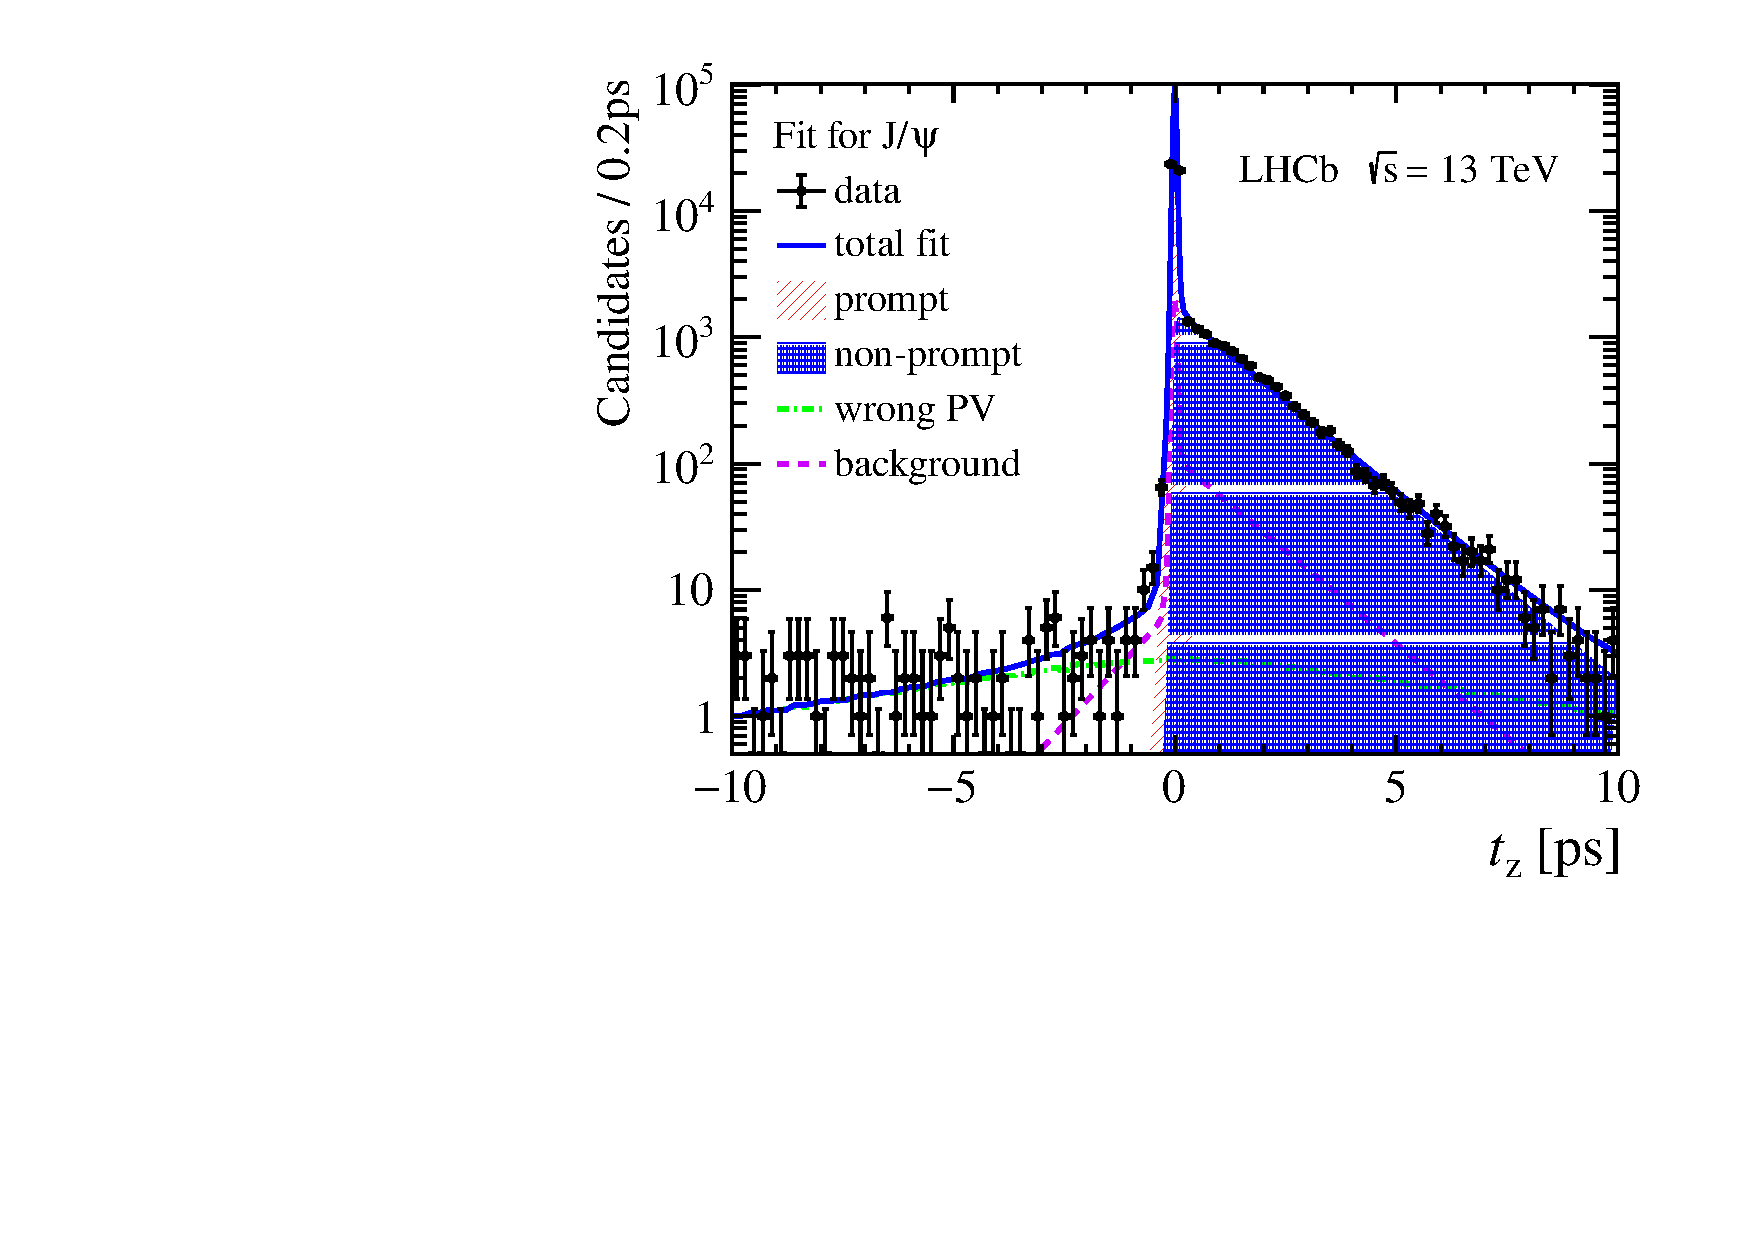
\includegraphics[width=0.49\linewidth]{pdf/Jpsi/2DFit/n1y2pt4.pdf}
     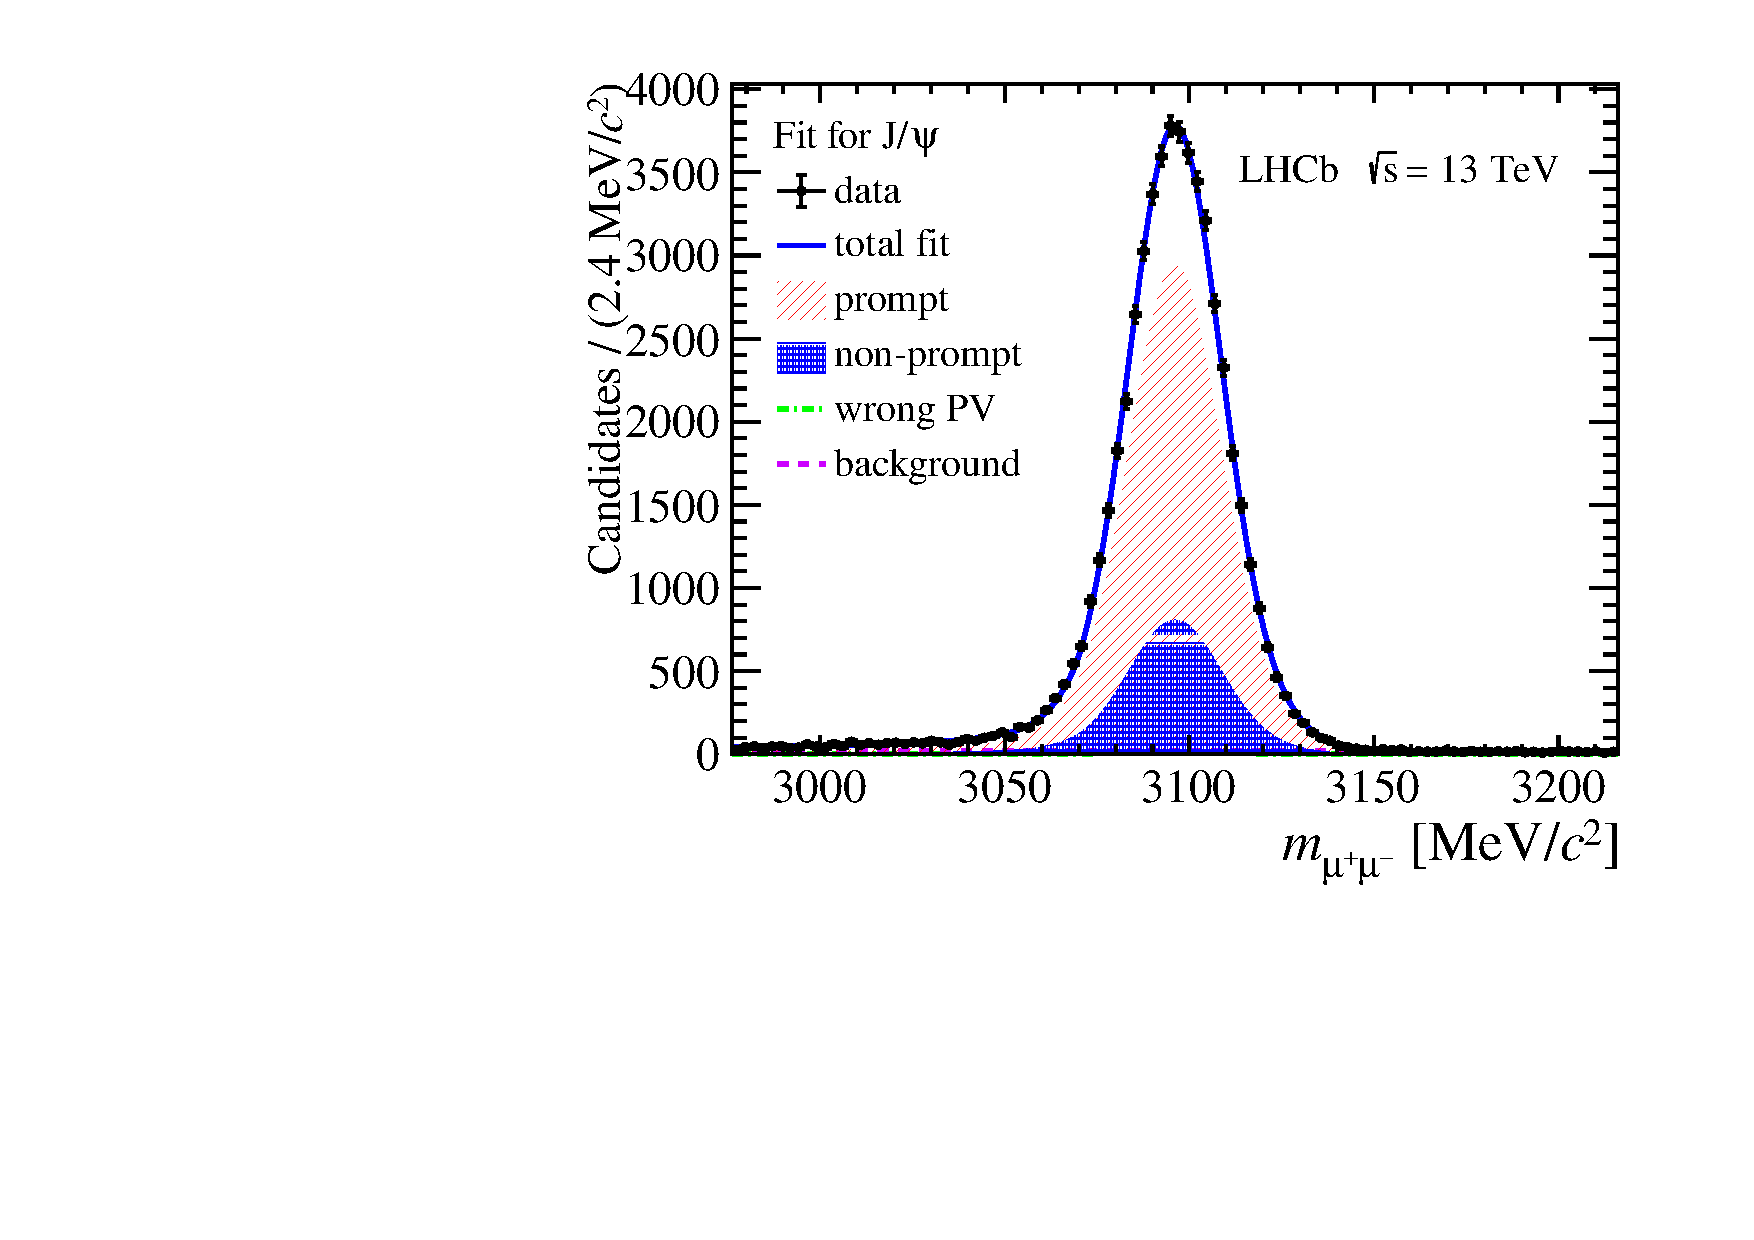
\includegraphics[width=0.49\linewidth]{pdf/Jpsi/drawmass/n1y2pt4.pdf}
     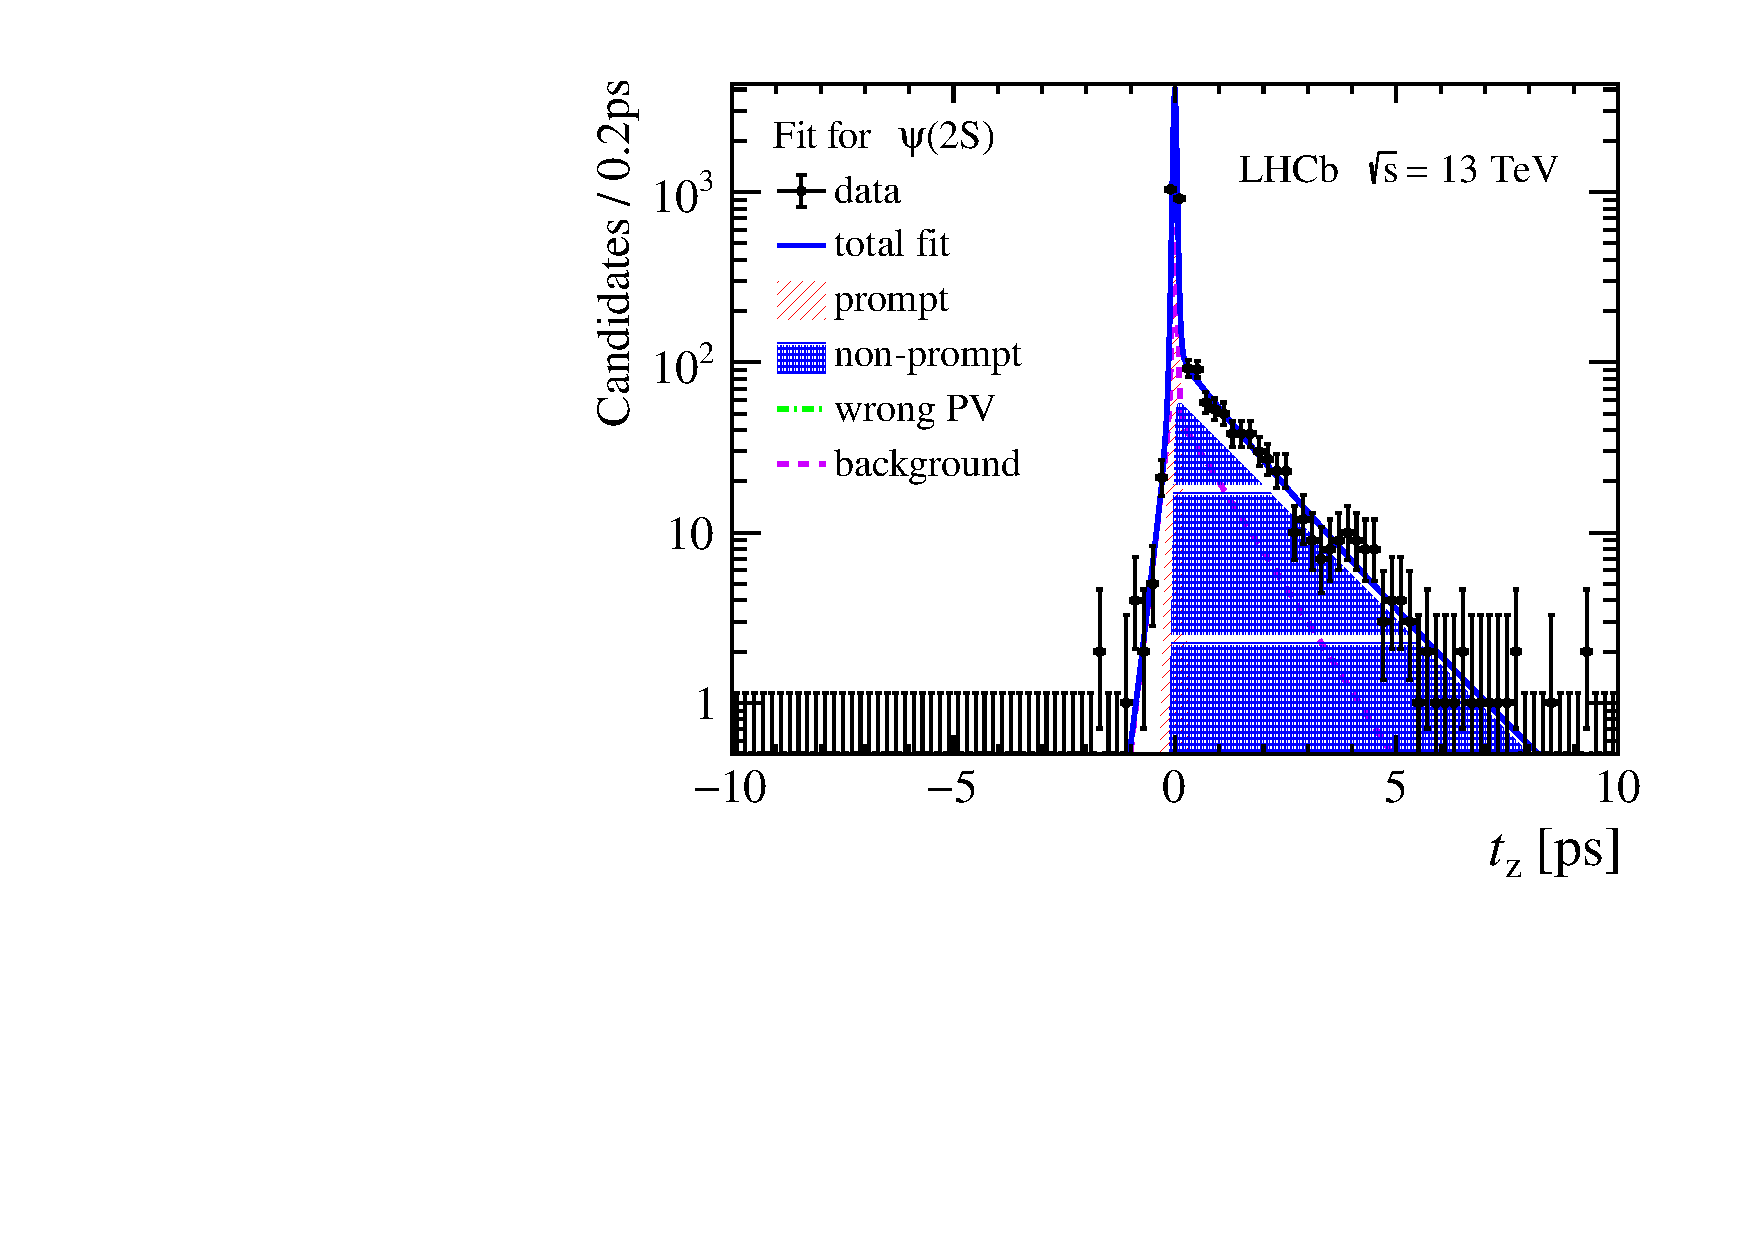
\includegraphics[width=0.49\linewidth]{pdf/Psi2S/2DFit/n1y2pt4.pdf}
     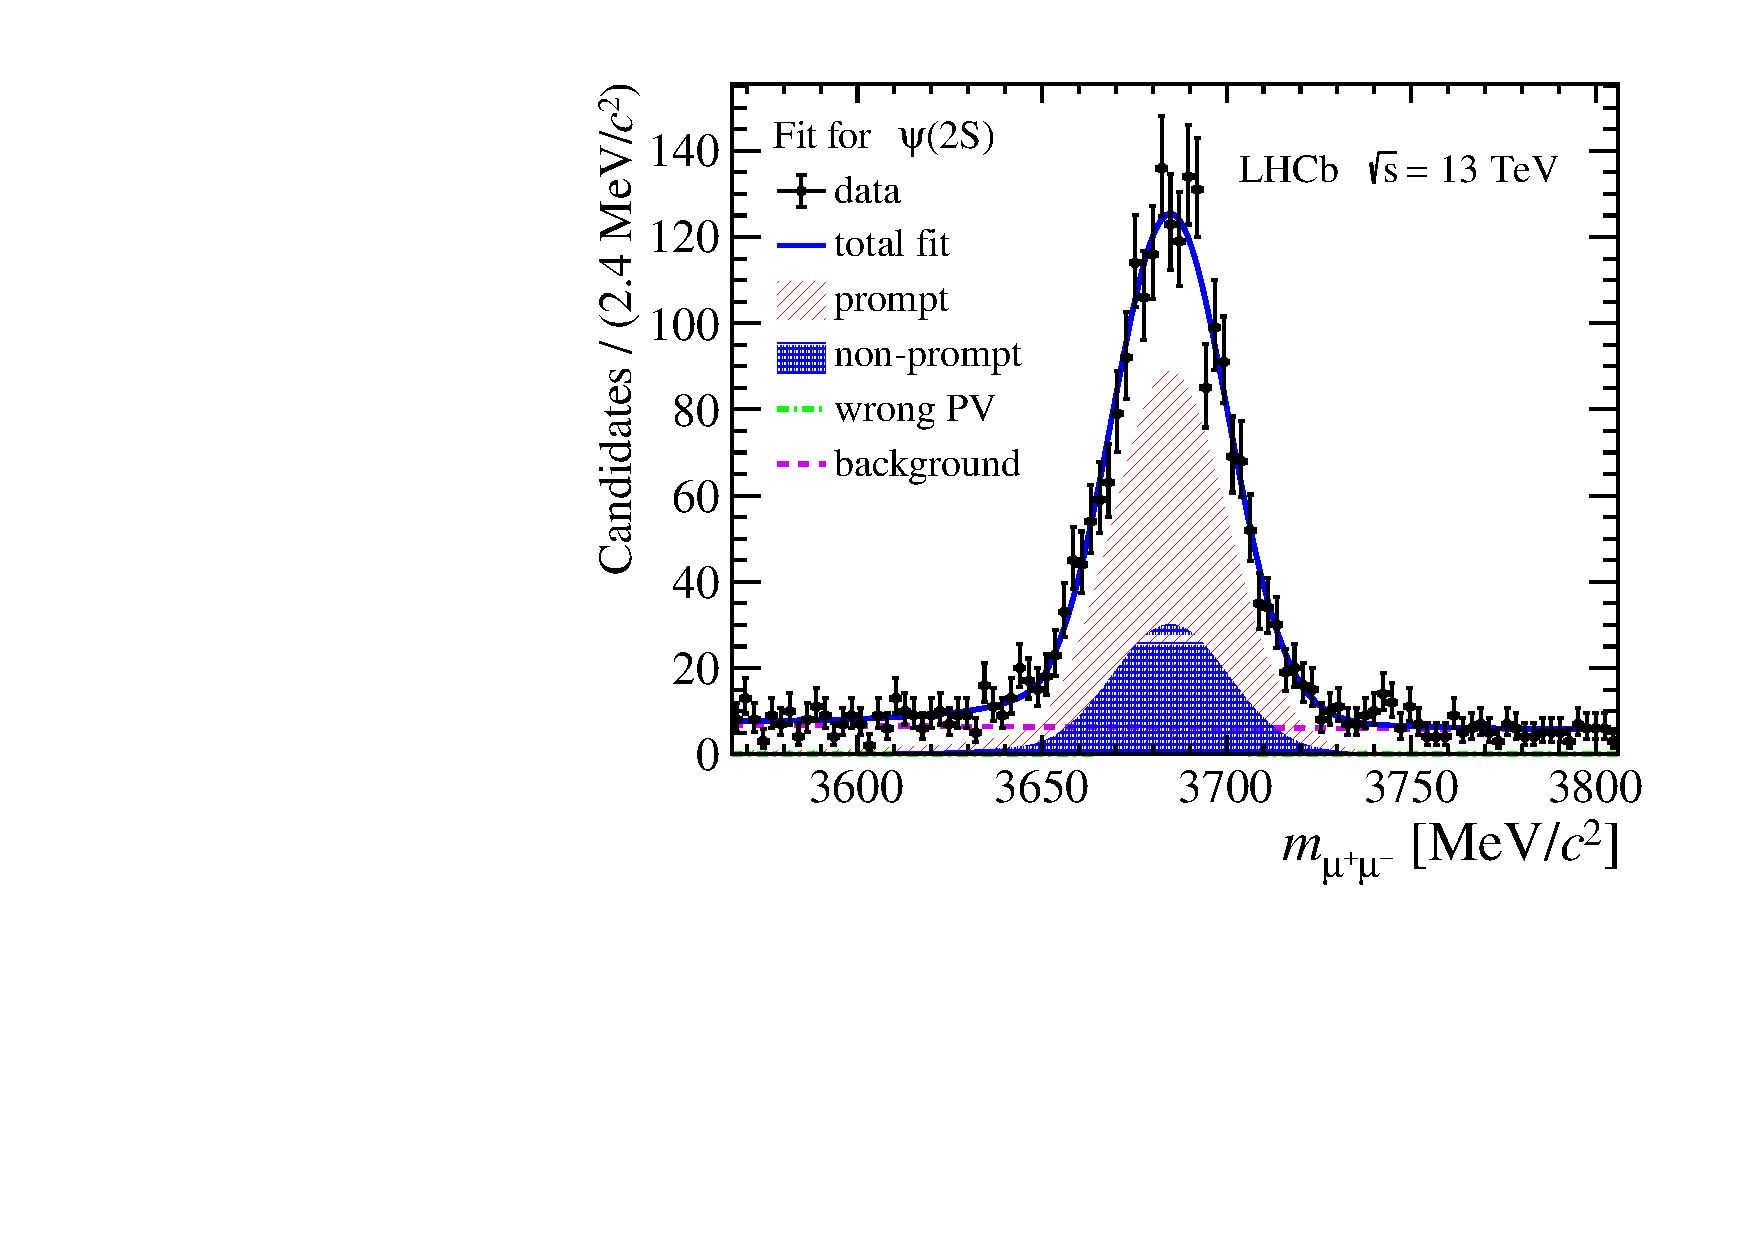
\includegraphics[width=0.49\linewidth]{pdf/Psi2S/drawmass/n1y2pt4.pdf}
   \end{center}
   \caption{
   Distributions of the (left) pseudo decay time and (right) mass for (upper) \jpsi and (lower) \psitwos are plotted in the region $4\leq N_{\rm tracks}^{\rm PV} < 20$, $2.8<y<3.5$, and $6<\pt<8\gevc$. The fit results are overlaid.
     }
   \label{fig:2Dtz}
 \end{figure}
The total efficiency \effTot is the product of the geometrical acceptance and the efficiencies of the particle reconstruction, event selection, muon identification and the trigger. The track reconstruction and muon identification efficiencies are determined using data-driven methods~\cite{Anderlini:2202412,LHCb-DP-2013-002}. The trigger efficiency is estimated on simulation and cross-checked using data~\cite{Tolk:2014llp}. The total efficiencies for prompt and non-prompt signals are calculated separately in each (\pt, $y$) and multiplicity bin. They are found to be very similar.
The efficiencies in different multiplicity regions are determined separately, according to the binning scheme in data samples.


%Systematic uncertainty
\section{Systematic uncertainties}
\def\effTri{\ensuremath{\epsilon_{\mathrm{trigger}}}\xspace}
\def\effTotJ{\ensuremath{\epsilon_{\mathrm{tot,\jpsi}}}\xspace}
\def\effTotP{\ensuremath{\epsilon_{\mathrm{tot,\psitwos}}}\xspace}
\def\pandb{prompt components and components from $b$-hadron decay}
Systematic uncertainties arising from a variety of sources are studied. The systematic uncertainty ranges for the ratios in different $N_{\rm tracks}^{\rm PV}$ bins are summarized in Table~\ref{SysU}. The binning scheme for multiplicity and (\pt, $y$) ensures that in each individual bin, analysis can be performed with enough events.

To study the uncertainties related to the mass fits, the signal invariant mass distribution in each bin is also fitted with a kernel-estimated~\cite{Cranmer:2000du} distribution extracted from simulated samples. In order to account for the difference in resolution between data and simulation, a Gaussian function is used to smear the shape of the signals. The study is performed in each kinematic and multiplicity bin, and the relative difference between the ratio obtained from the default fit model and from the alternative fit model is quoted as a systematic uncertainty for both the prompt and non-prompt ratios.

To estimate the uncertainty due to imperfection of the $t_z$ signal model, it is fitted to the simulated sample, where the true numbers of prompt and non-prompt candidates are known. Then the fit yield is compared to the true numbers and the variation is quoted as a systematic uncertainty. For the $t_z$ background model, the sideband sample which the model is originally fitted to, is replaced by the distribution extracted from the data using the $sPlot$~\cite{Pivk:2004ty} method. The invariant mass and pseudo decay time have a correlation factor of $10^{-3}$, so the invariant mass may be used as a discriminating variable to extract the signal and background distribution of pseudo decay time $t_z$ with the $sPlot$~\cite{Pivk:2004ty} method. The difference between the alternative and default fits is taken as a systematic uncertainty.


The tracking efficiencies are determined from the simulation. Corrections, as a function of $p$ and $\eta$, are determined using \jpsi control samples in data~\cite{DeCian:1402577}. The uncertainty due to the limited size of the control samples are propagated to the results using pseudoexperiments. The multiplicity distribution of simulated samples is weighted to match that of the control samples, and the bias caused by the choice of the multiplicity variable is canceled in the \psitwos-to-\jpsi cross-section production ratio.

The muon identification efficiency is obtained using simulated samples and calibrated with data samples of $\jpsi\rightarrow \mu^+\mu^-$ decays using the tag-and-probe method~\cite{Archilli:2013npa}.  The single-muon identification efficiency is calculated as a function of $p$, $\eta$ and the number of hits in the SPD, $N_{\rm spd}$. The uncertainty due to the limited size of control samples is propagated to the final result. The uncertainty related to the binning scheme is studied by changing the binning scheme of ($p$,$\eta$,$N_{\rm spd}$), and the variation on the ratio of production is quoted as a systematic uncertainty.

The uncertainty due to limited size of the simulated sample used to determine the efficiencies is propagated to the final result. The trigger efficiency is estimated from simulation and is cross-checked by a data-driven method using a fully reconstructed sample. The trigger efficiency in data is determined using a subset of events that would have triggered independently of the \jpsi and \psitwos signal candidates~\cite{LHCb-DP-2012-004}. The relative difference between data and simulation in different multiplicity bins is taken as a systematic uncertainty.
The uncertainties in the charmonium branching ratios and luminosity cancel in the normalised ratios, defined as the ratios in different multiplicity regions divided by the total ratio over all multiplicity regions.
\begin{table}[!tbp]
  \centering
	\caption{Summary of systematic uncertainty ranges for the double-differential \psitwos-to-\jpsi cross-section ratio, in different kinematic bins within corresponding multiplicity intervals in $\%$. Sources marked with $\dagger$ are considered to be correlated beween bins.}
\begin{center}
  \begin{tabular}{l|ccccc}
    \hline
    & \multicolumn{5}{c}{Interval of $N_{\rm tracks}^{\rm PV}$}\\
    Source &  4--20 & 20--45  & 45--70   & 70--95   & 95--200   \\ \hline
    Signal mass shape$\dagger$ & & & & &  \\
    prompt \& non-prompt & 0.1--1.6 & 0.1--1.3 & 0.1--1.1 & 0.1--1.8 & 0.1--3.2 \\ \hline
    Signal $t_z$ shape$\dagger$  & & & & &  \\
    prompt & 0.2--1.8 & 0.2--1.2 & 0.0--1.4 & 0.0--1.8 & 0.1--9.7 \\ 
    non-prompt & 0.0--1.8 & 0.2--2.0 & 0.0--2.3 & 0.1--1.7 & 0.0--4.0 \\ \hline
    Background $t_z$ shape$\dagger$  & & & & &  \\
    prompt & 0.0--1.6 & 0.2--3.1 & 0.0--2.2 & 0.2--6.2 & 0.4--6.4 \\
    non-prompt & 1.2--6.5 & 0.2--5.1 & 0.2--3.4 & 0.6--3.7 & 0.0--9.7 \\ \hline
    Tracking efficiency$\dagger$ & & & & &  \\
    prompt & 0.0--0.8 & 0.0--0.7 & 0.0--0.7 & 0.0--0.7 & 0.0--0.8 \\
    non-prompt & 0.0--1.0 & 0.0--1.1 & 0.0--1.2 & 0.0--1.1 & 0.0--1.1 \\ \hline
    Trigger efficiency$\dagger$ & & & & &  \\
    prompt \& non-prompt & 2.1 & 4.0 & 1.0 & 0.0 & 1.1 \\ \hline
    Muon ID sample size$\dagger$ & & & & &  \\
    prompt & 0.0--0.1 & 0.0--0.1 & 0.0--0.1 & 0.0--0.1 & 0.0--0.1 \\
    non-prompt & 0.0--0.1 & 0.0--0.1 & 0.0--0.1 & 0.0--0.1 & 0.0--0.1 \\
    Muon ID binning$\dagger$ & & & & &  \\
    prompt & 0.1--0.8 & 0.1--0.8 & 0.1--0.9 & 0.1--0.7 & 0.1--0.9 \\
    non-prompt & 0.0--0.9 & 0.0--0.8 & 0.1--0.7 & 0.1--0.8 & 0.1--1.0 \\ \hline
    Simulated sample size & & & & &  \\
    prompt & 1.5--4.4 & 1.1--2.4 & 1.3--2.5 & 2.0--3.4 & 4.0--6.4 \\
    non-prompt & 2.7--5.5 & 1.6--3.2 & 1.6--3.4 & 2.3--4.7 & 4.1--8.9 \\ \hline
    Total & & & & &  \\
    prompt & 3.1--7.7 & 4.3--5.5 & 2.2--3.9 & 2.9--7.7 & 6.1--13 \\
    non-prompt &5.2--10.2 & 5.0--7.6 & 3.3--5.3 & 3.9--8.4 & 7.4--17\\ \hline
\end{tabular}
\end{center}
\label{SysU}
\end{table}

The \psitwos-to-\jpsi cross-section ratios are reported with integration separately over \pt and $y$, and over the full \pt and $y$ range. The systematic uncertainties that are correlated across different bins may cancel each other when adding the production over different kinematic bins, since in some bins the production cross-section may be over-estimated and in other bins it may be under-estimated. The systematic uncertainties for ratios over integrated kinematic bins are obtained in the same way as for each bins. The uncertainties that are not correlated across different bins are propagated to the final result.

%Result:
\section{Results}
\label{sec:results}

\subsection{\boldmath{\psitwos-to-\jpsi} ratio as a function of multiplicity}
The measured \psitwos-to-\jpsi production cross-section ratios are presented in various kinematic and multiplicity bins, with the full numerical data details provided in Appendix A~\ref{Sec:Ratio}. 
Subsequently, the normalised ratio as a function of the nondimensionalised multiplicity can be obtained by integrating the double-differential results over the \pt and $y$ bins. The \psitwos-to-\jpsi ratio in each multiplicity bin is normalised to the ratio of total cross-section of \jpsi and \psitwos mesons as
\begin{equation}
\mathrm{Normalised \ } \sigma_{\psitwos,n}/\sigma_{\jpsi,n}=\frac{\sigma_{\psitwos,n}/\sigma_{\jpsi,n}}{\sum_n\sigma_{\psitwos,n}/\sum_n\sigma_{\jpsi,n}},
\label{norm}
\end{equation}
where $n$ is the bin index for multiplicity.
The normalised ratio for the integrated production over \pt and $y$ as a function of the nondimensionalised $N_{\rm tracks}^{\rm PV}$ is illustrated in Fig.~\ref{Ratio}. The multiplicity distribution for \jpsi and \psitwos are quite similar to each other, and the $x$-values are the weighted average of (non-)prompt \jpsi and \psitwos multiplicity in each bin, where the weight is the inverse variation of the multiplicity distribution in corresponding bin. The uncertainty for the $x$-values is nearly negligible. For the sake of visibility, a small width is applied when drawing the systematic uncertainty.

The production ratio from $b$-hadron decays shows little dependence on multiplicity irrespective of the choice of multiplicity variable. For prompt \psitwos and \jpsi,  an evident decrease of ratio with $N_{\rm tracks}^{\rm PV}$ is observed (P-value of slope $<0.0005$), which aligns well with the predictions of the co-mover model, except in the low multiplicity region.
\begin{figure}[H]
    \begin{center}
      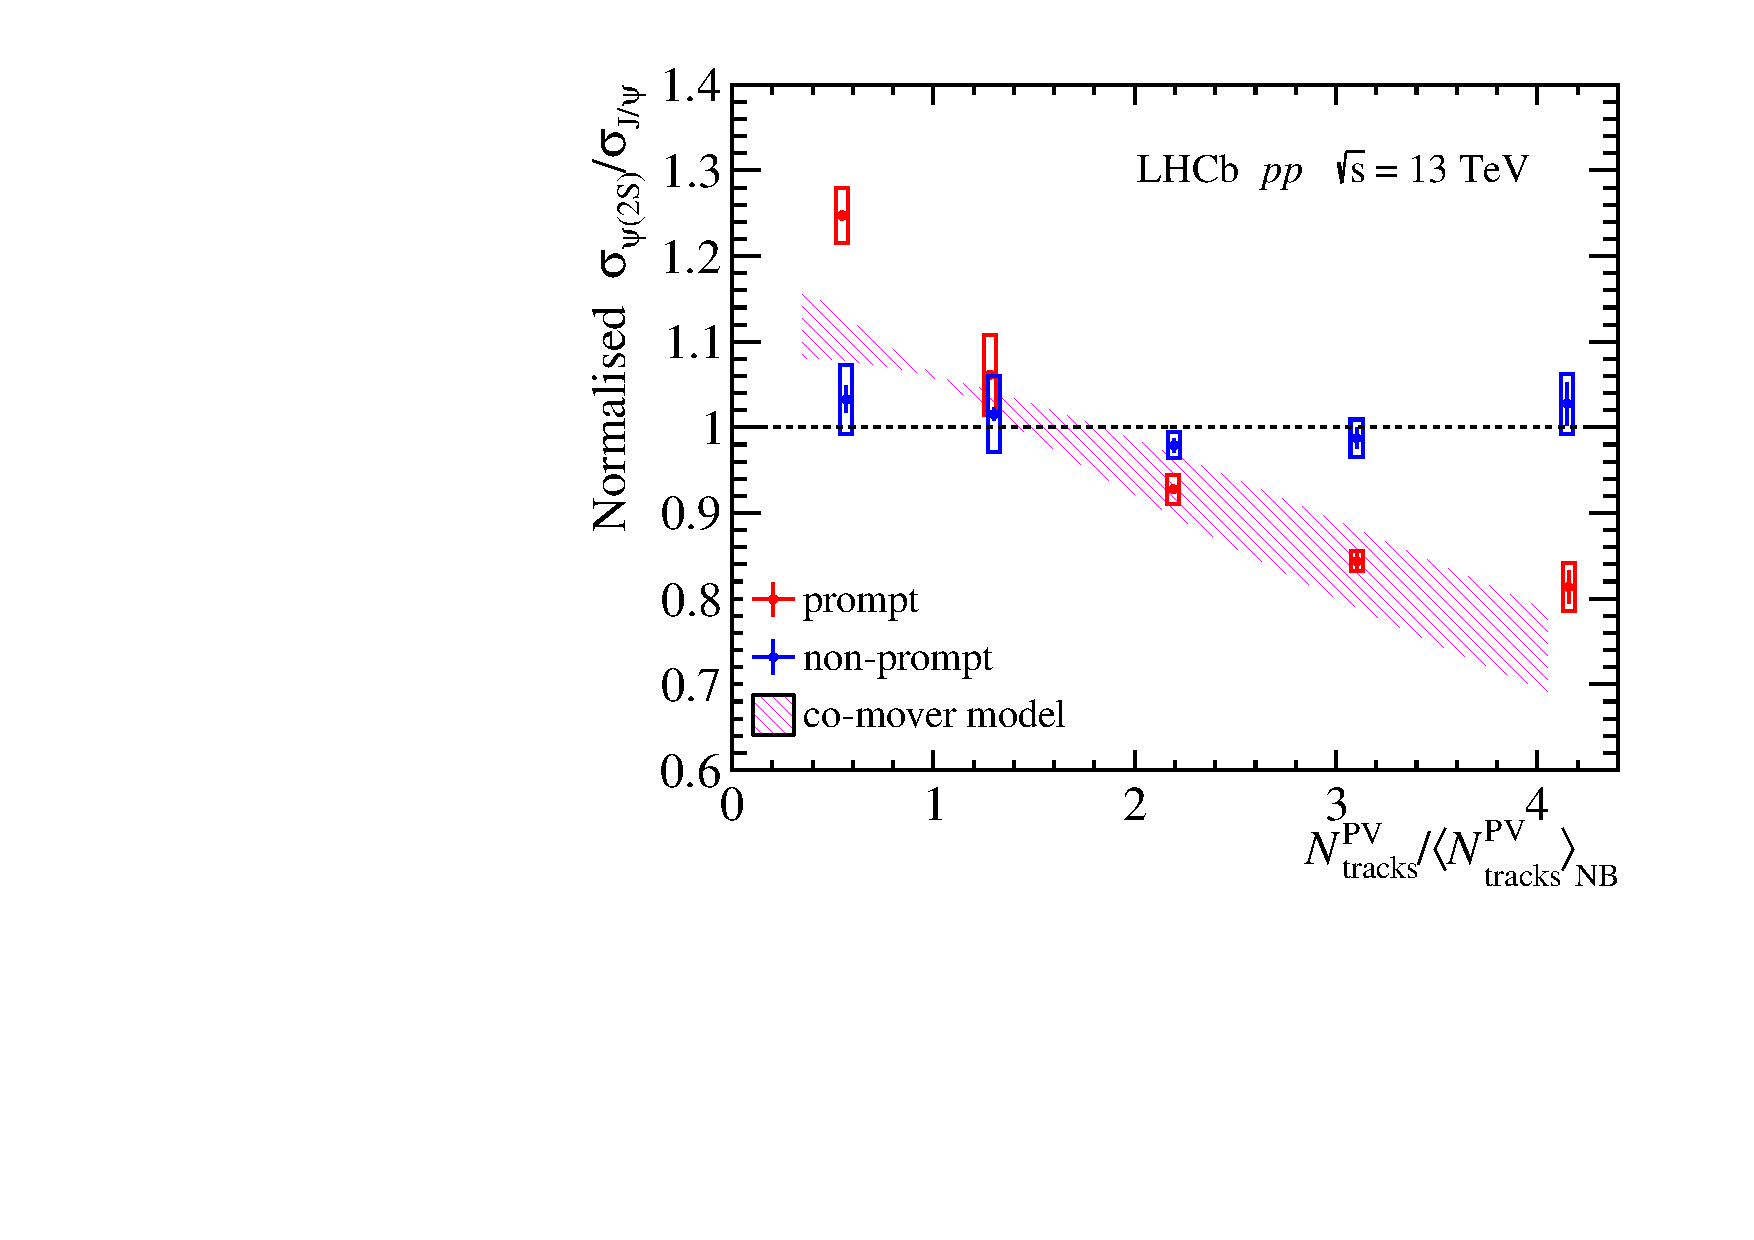
\includegraphics[width=0.6\linewidth]{pdf/Result/All.pdf}
    \end{center}
	\caption{Normalised production ratio as a function of $N_{\rm tracks}^{\rm PV}/\langle N_{\rm tracks}^{\rm PV}\rangle_{\rm{NB}}$, integrated over the full \pt-$y$ range of $2.0<y<4.5$ and $0.3<\pt<20$~\gevc with $-60 < z_{\rm PV} < 180$~mm. The error bars represent statistical uncertainties and heights of the boxes represent systematical uncertainties. 
      }
    \label{Ratio}
\end{figure}

Additionally, the ratios are examined as a function of the nondimensionalised $N_{\rm bwd}^{\rm PV}$ and $N_{\rm fwd}^{\rm PV}$ in Fig.~\ref{RatioFB}. 
\begin{figure}[H]
  \begin{center}
    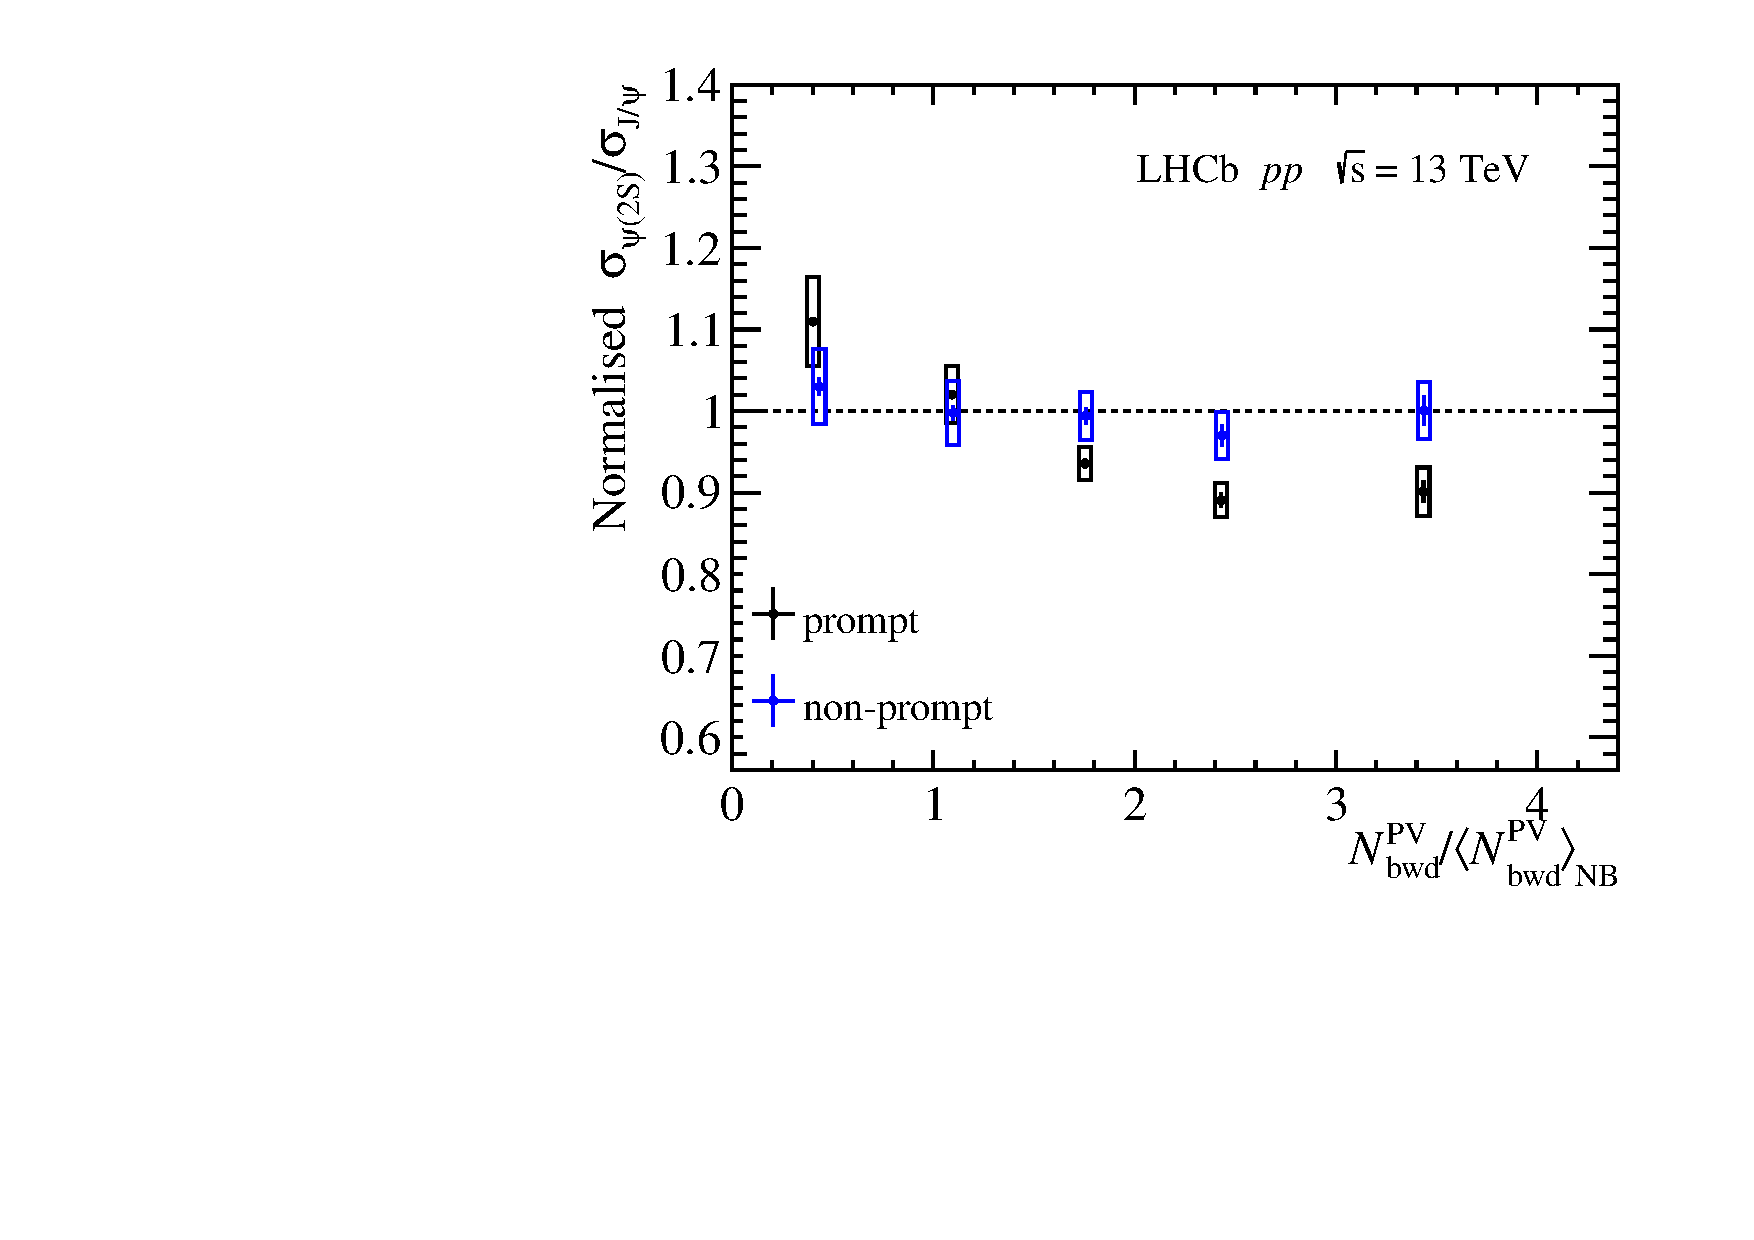
\includegraphics[width=0.49\linewidth]{pdf/Result/AllB.pdf}
    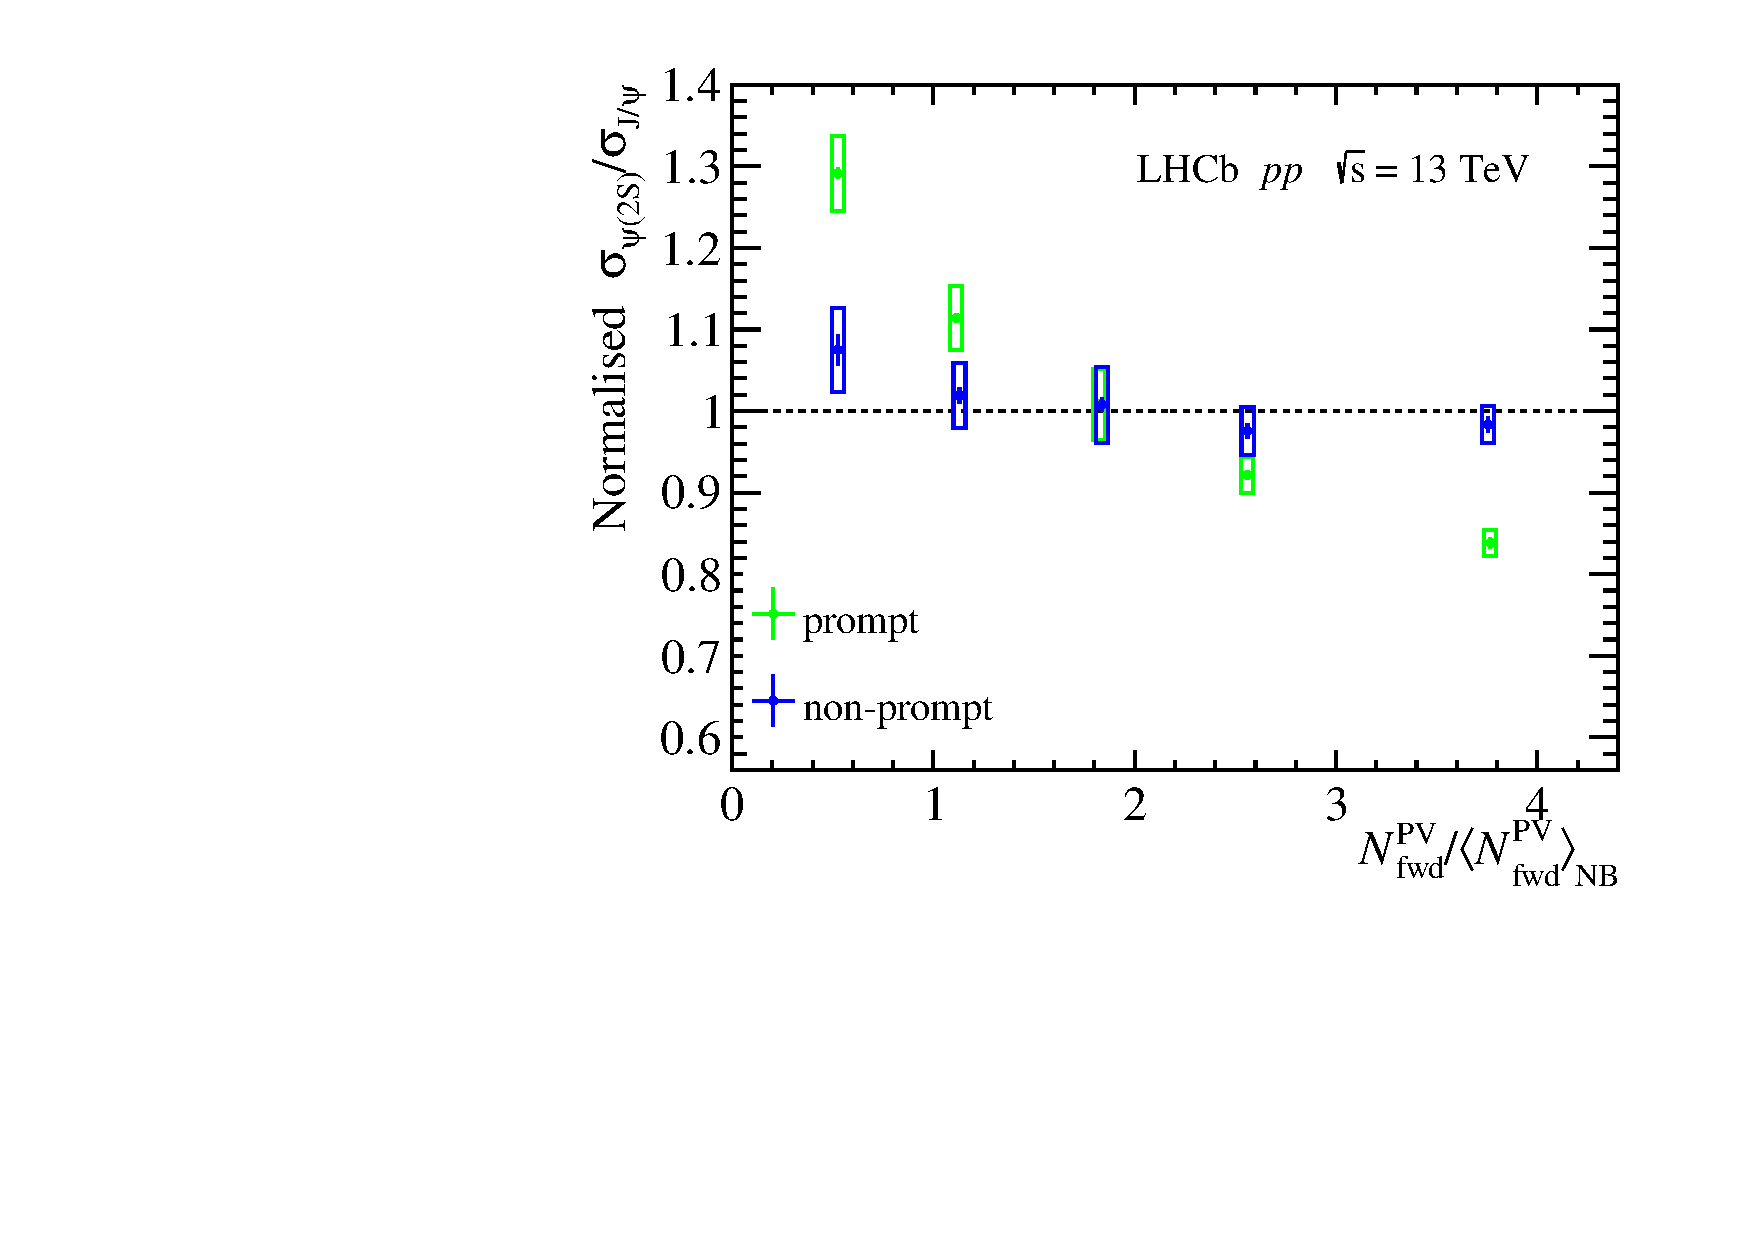
\includegraphics[width=0.49\linewidth]{pdf/Result/AllF.pdf}
    \vspace*{-0.5cm}
  \end{center}
	\caption{Normalised production ratio as a function of (left) $N_{\rm bwd}^{\rm PV}/\langle N_{\rm bwd}^{\rm PV}\rangle_{\rm{NB}}$ , with $-30<z_{\rm PV}<180$~mm, and (right) $N_{\rm fwd}^{\rm PV}/\langle N_{\rm fwd}^{\rm PV}\rangle_{\rm{NB}}$, with $-180<z_{\rm PV}<180$~mm, integrated over the full \pt-$y$ range of $2.0<y<4.5$ and $0.3<\pt<20$~\gevc.
    }
  \label{RatioFB}
\end{figure}
Notably, the trend is weaker as a function of $N_{\rm bwd}^{\rm PV}$ than $N_{\rm fwd}^{\rm PV}$ and  $N_{\rm tracks}^{\rm PV}$. This suggests a correlation between the relative suppression and local particle multiplicity. According to comover effect~\cite{Ferreiro:2012rq}, the ratio should remain constant across different $N_{\rm bwd}^{\rm PV}$, with $N_{\rm bwd}^{\rm PV}$ being measured in a backward rapidity range and not including the muon tracks from charmonia. The slight decreasing trend of ratio as function of $N_{\rm bwd}^{\rm PV}$ could result from the correlation between $N_{\rm bwd}^{\rm PV}$ and $N_{\rm fwd}^{\rm PV}$, where the correlation factor is 0.54 and 0.51 for prompt \jpsi and \psitwos, respectively. To estimate the impact of this correlation, the mean $N_{\rm fwd}^{\rm PV}$ value within each $N_{\rm bwd}^{\rm PV}$ bin for prompt charmonia is calculated. Then, the normalised ratios across different $N_{\rm bwd}^{\rm PV}$ bins are plotted as a function of $N_{\rm fwd}^{\rm PV}$, as shown in Fig.~\ref{BtoF}. A coherent alignment in the decreasing trend is consistent with the hypothesis that the dependency of the normalised \psitwos-to-\jpsi ratio on $N_{\rm bwd}^{\rm PV}$ arises from $N_{\rm bwd}^{\rm PV}$-$N_{\rm fwd}^{\rm PV}$ correlation. 
\begin{figure}[H] 
    \begin{center}
      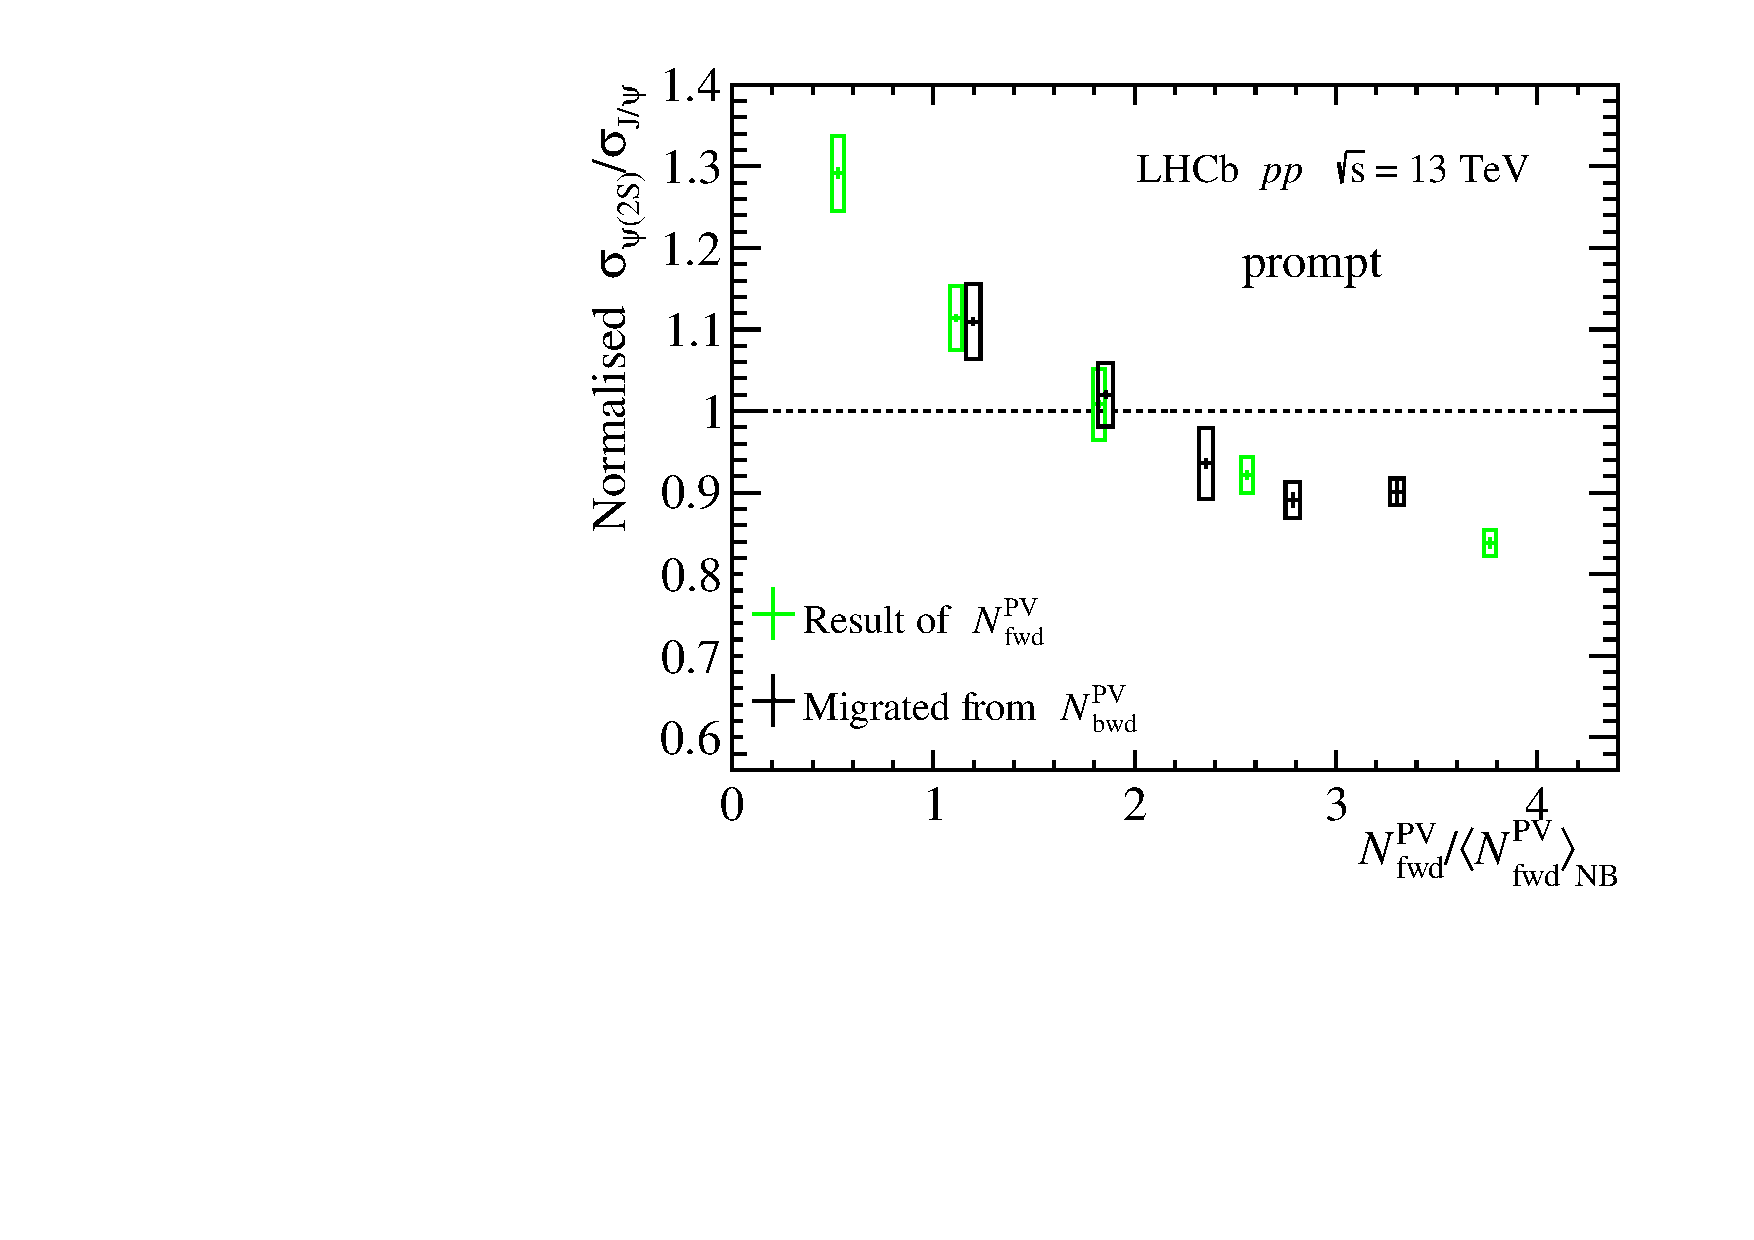
\includegraphics[width=0.6\linewidth]{pdf/Result/AllBtoF.pdf}
    \end{center}
	\caption{Normalised production ratio as a function of $N_{\rm fwd}^{\rm PV}/\langle N_{\rm fwd}^{\rm PV}\rangle_{\rm{NB}}$, compared to a translation of the ratio as a function of $N_{\rm bwd}^{\rm PV}/\langle N_{\rm bwd}^{\rm PV}\rangle_{\rm{NB}}$.
      } 
    \label{BtoF}
\end{figure}

\subsection{\boldmath{\psitwos-to-\jpsi} ratio in different \pt and $y$ ranges}
Figures~\ref{RatioPT_PVN},~\ref{RatioPT_For}, and~\ref{RatioPT_Back} present the normalised production ratios, as a function of the multiplicity, in different \pt ranges. The mean values for multiplicity variables in each bin are calculated in different kinematic regions accordingly, where their distributions are slight different. The relative production of \psitwos mesons is suppressed in the lower \pt region. However, in the high-\pt region, the prompt is almost independent of multiplicity as the non-prompt ratio. This is consistent with the measurement on multiplicity dependence of $\it{\Upsilon}(nS)$ by CMS~\cite{CMS:2020fae} and ATLAS~\cite{ATLAS-CONF-2022-023}, where the decreasing trend become slight in the high-\pt region.


\begin{figure}[H]
  \begin{center}

	  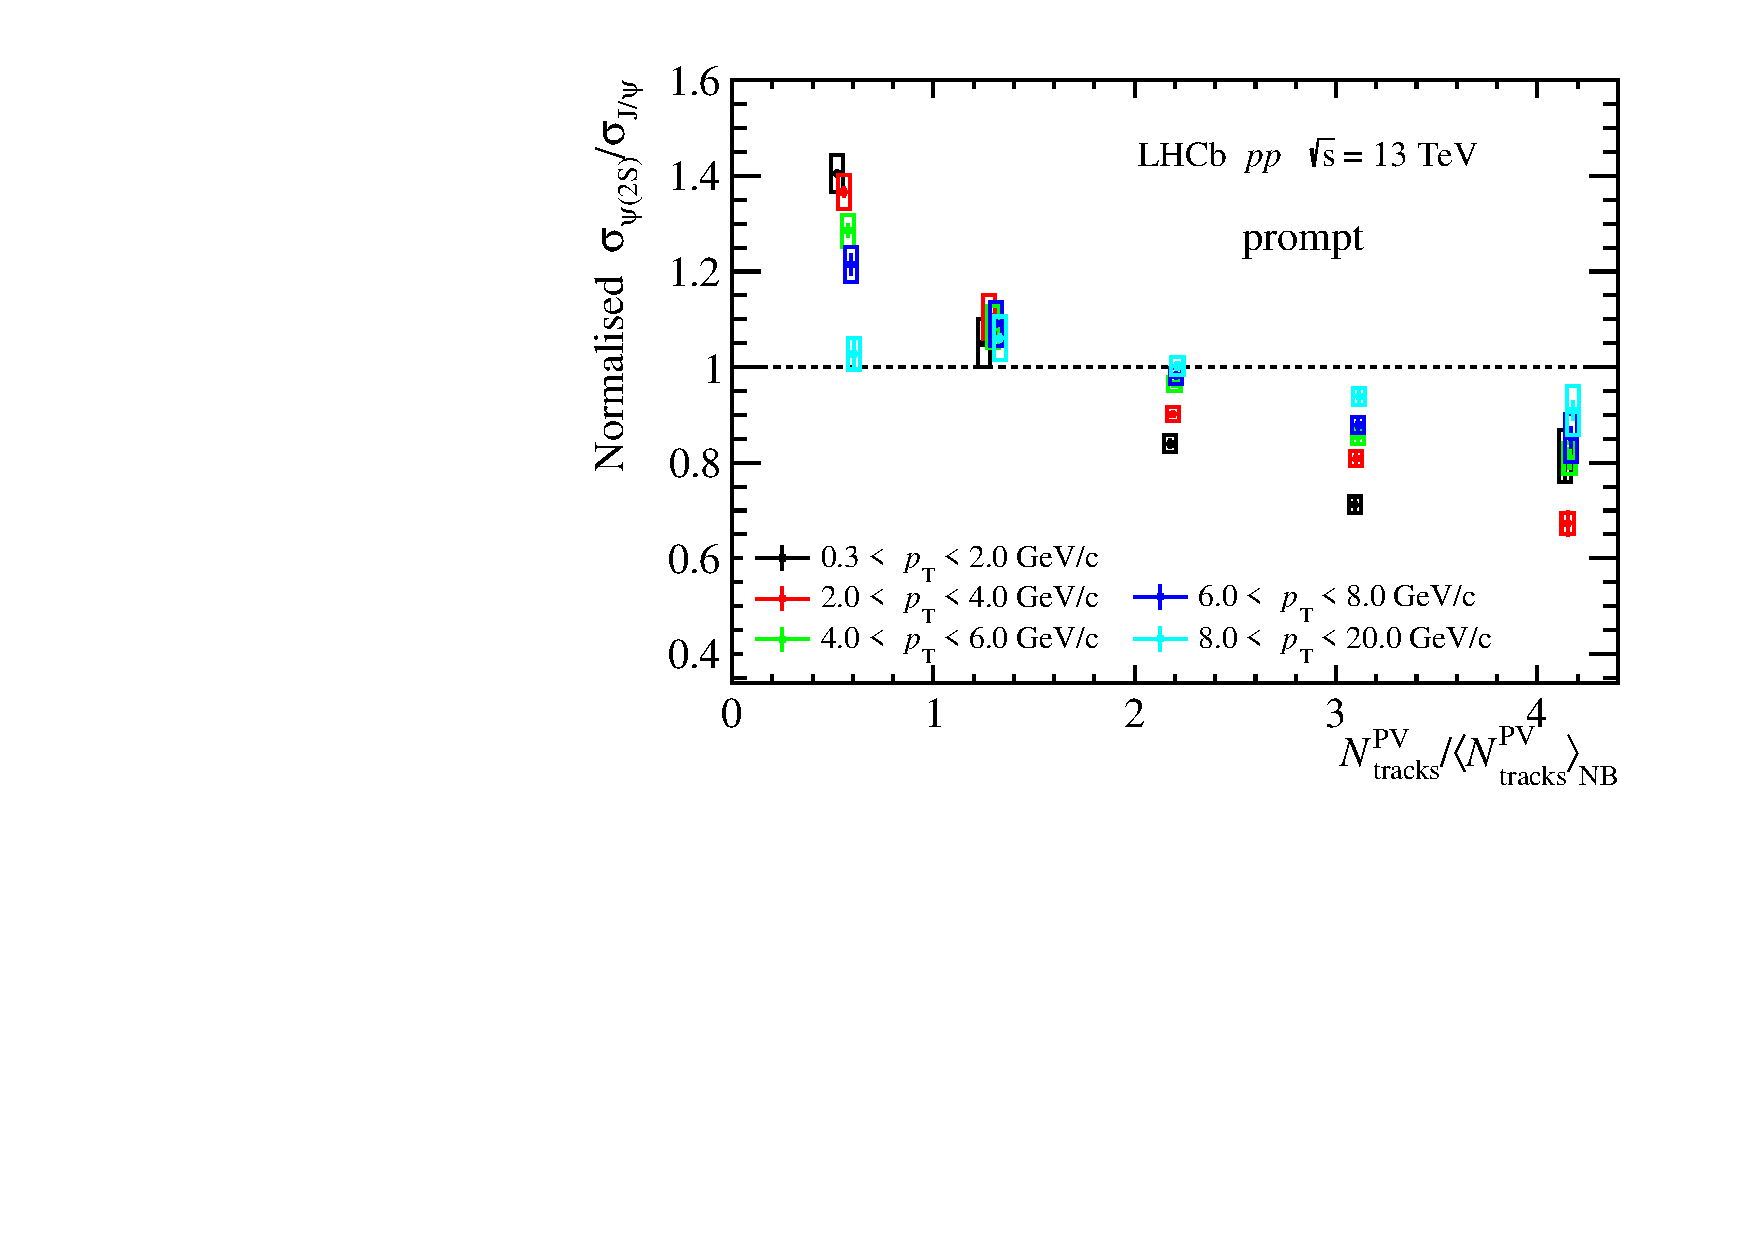
\includegraphics[width=0.48\linewidth]{pdf/Result/promptRatioPT.pdf}
          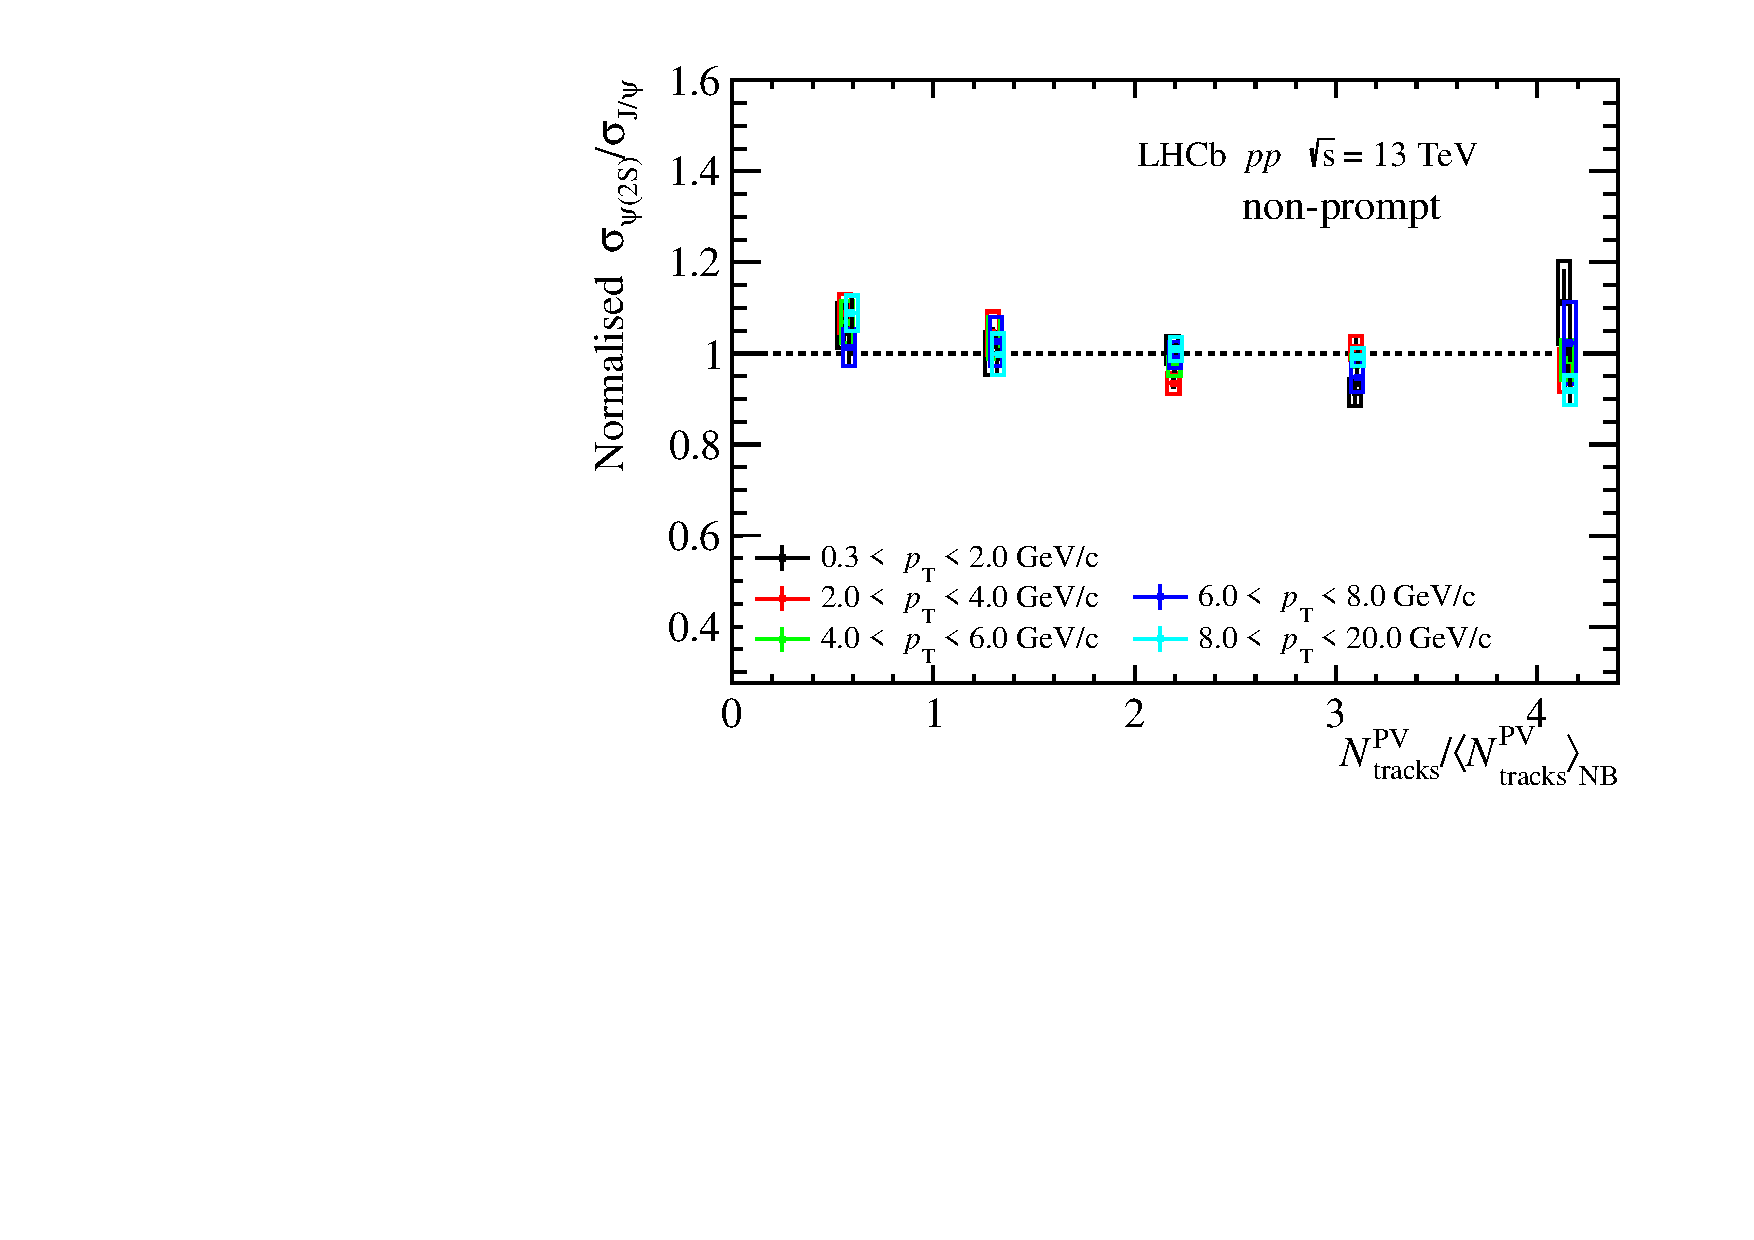
\includegraphics[width=0.48\linewidth]{pdf/Result/frombRatioPT.pdf}
	  \vspace*{-0.5cm}
  \end{center}
	\caption{Normalised production ratio for (left) prompt and(right) non-prompt charmonia as a function of $N_{\rm tracks}^{\rm PV}/\langle N_{\rm tracks}^{\rm PV}\rangle_{\rm{NB}}$ in different \pt intervals.}
  \label{RatioPT_PVN}
\end{figure}
\begin{figure}[H]
  \begin{center}
	  \vspace*{-0.5cm}
    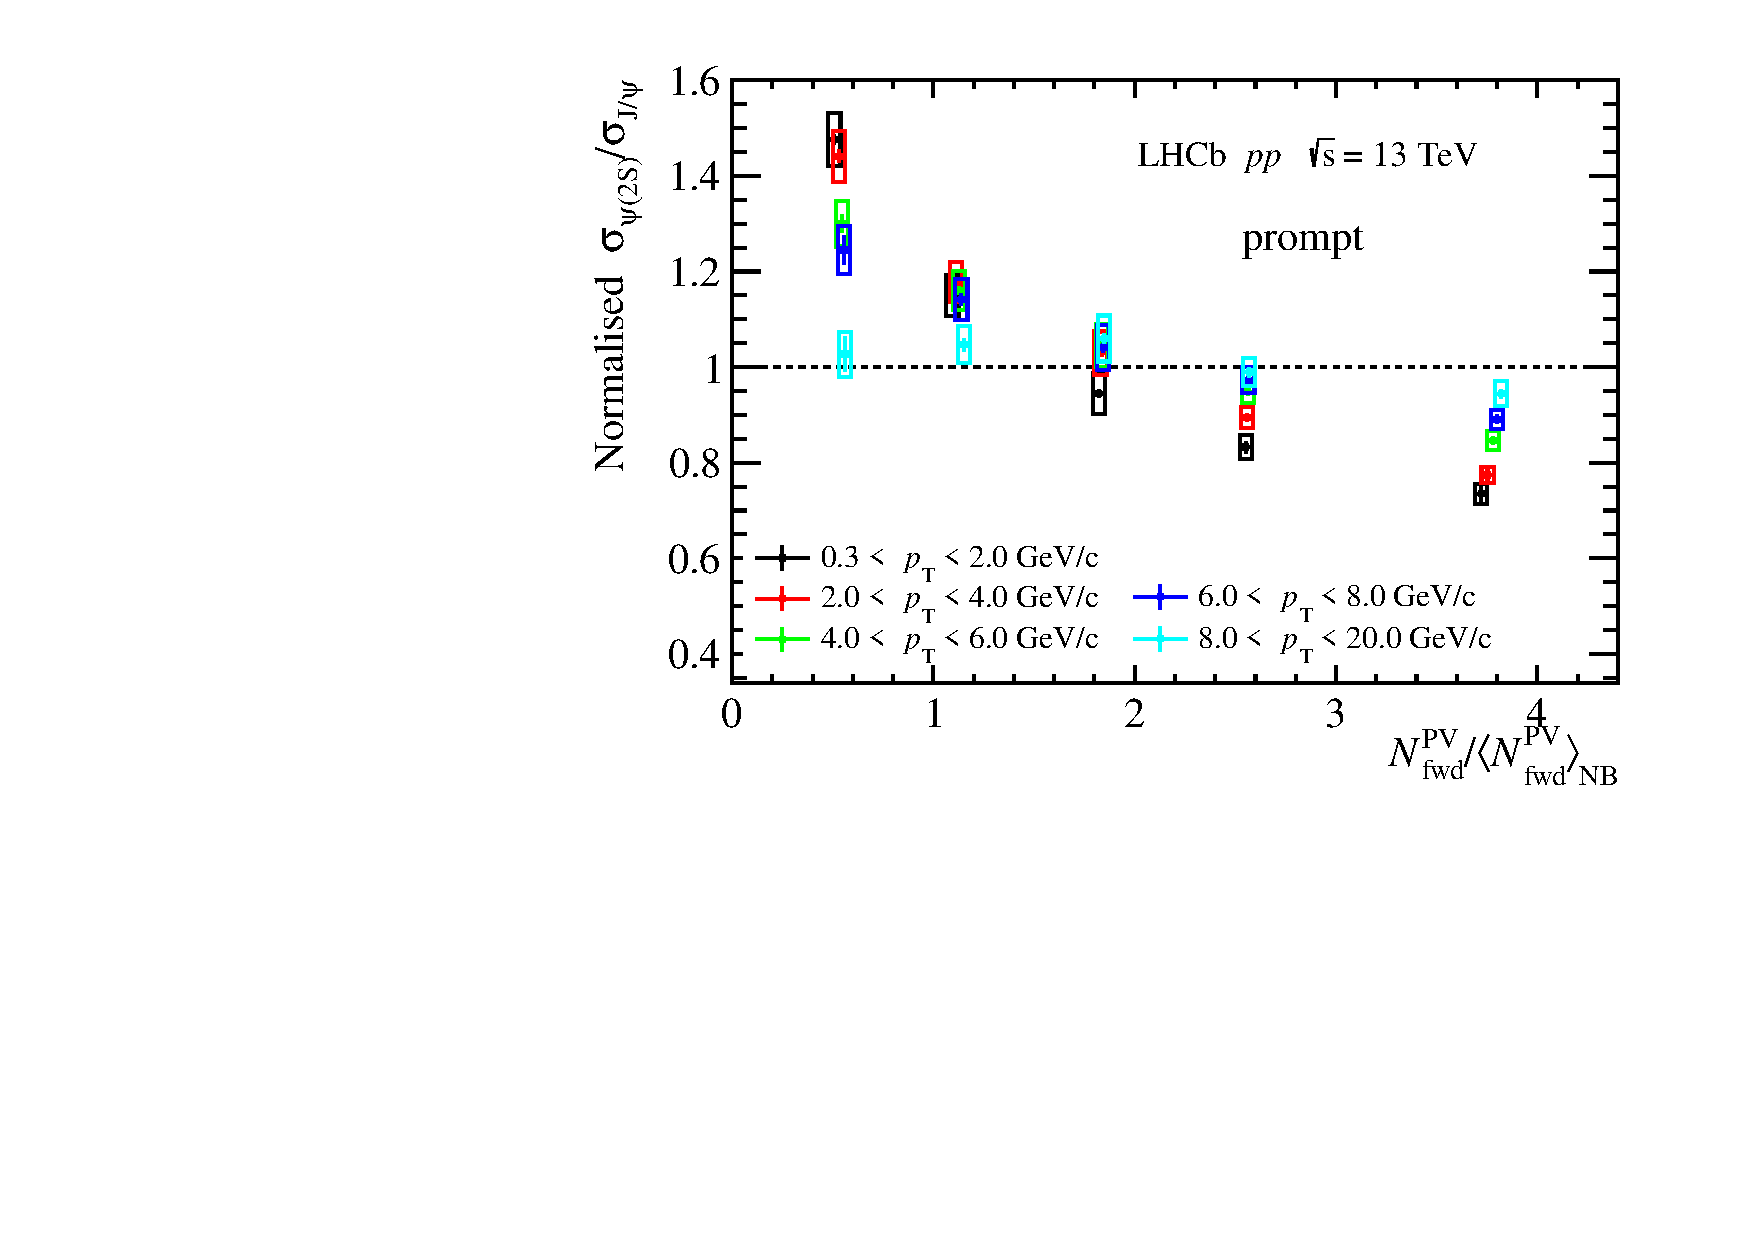
\includegraphics[width=0.48\linewidth]{pdf/Result/promptRatioPTF.pdf}
    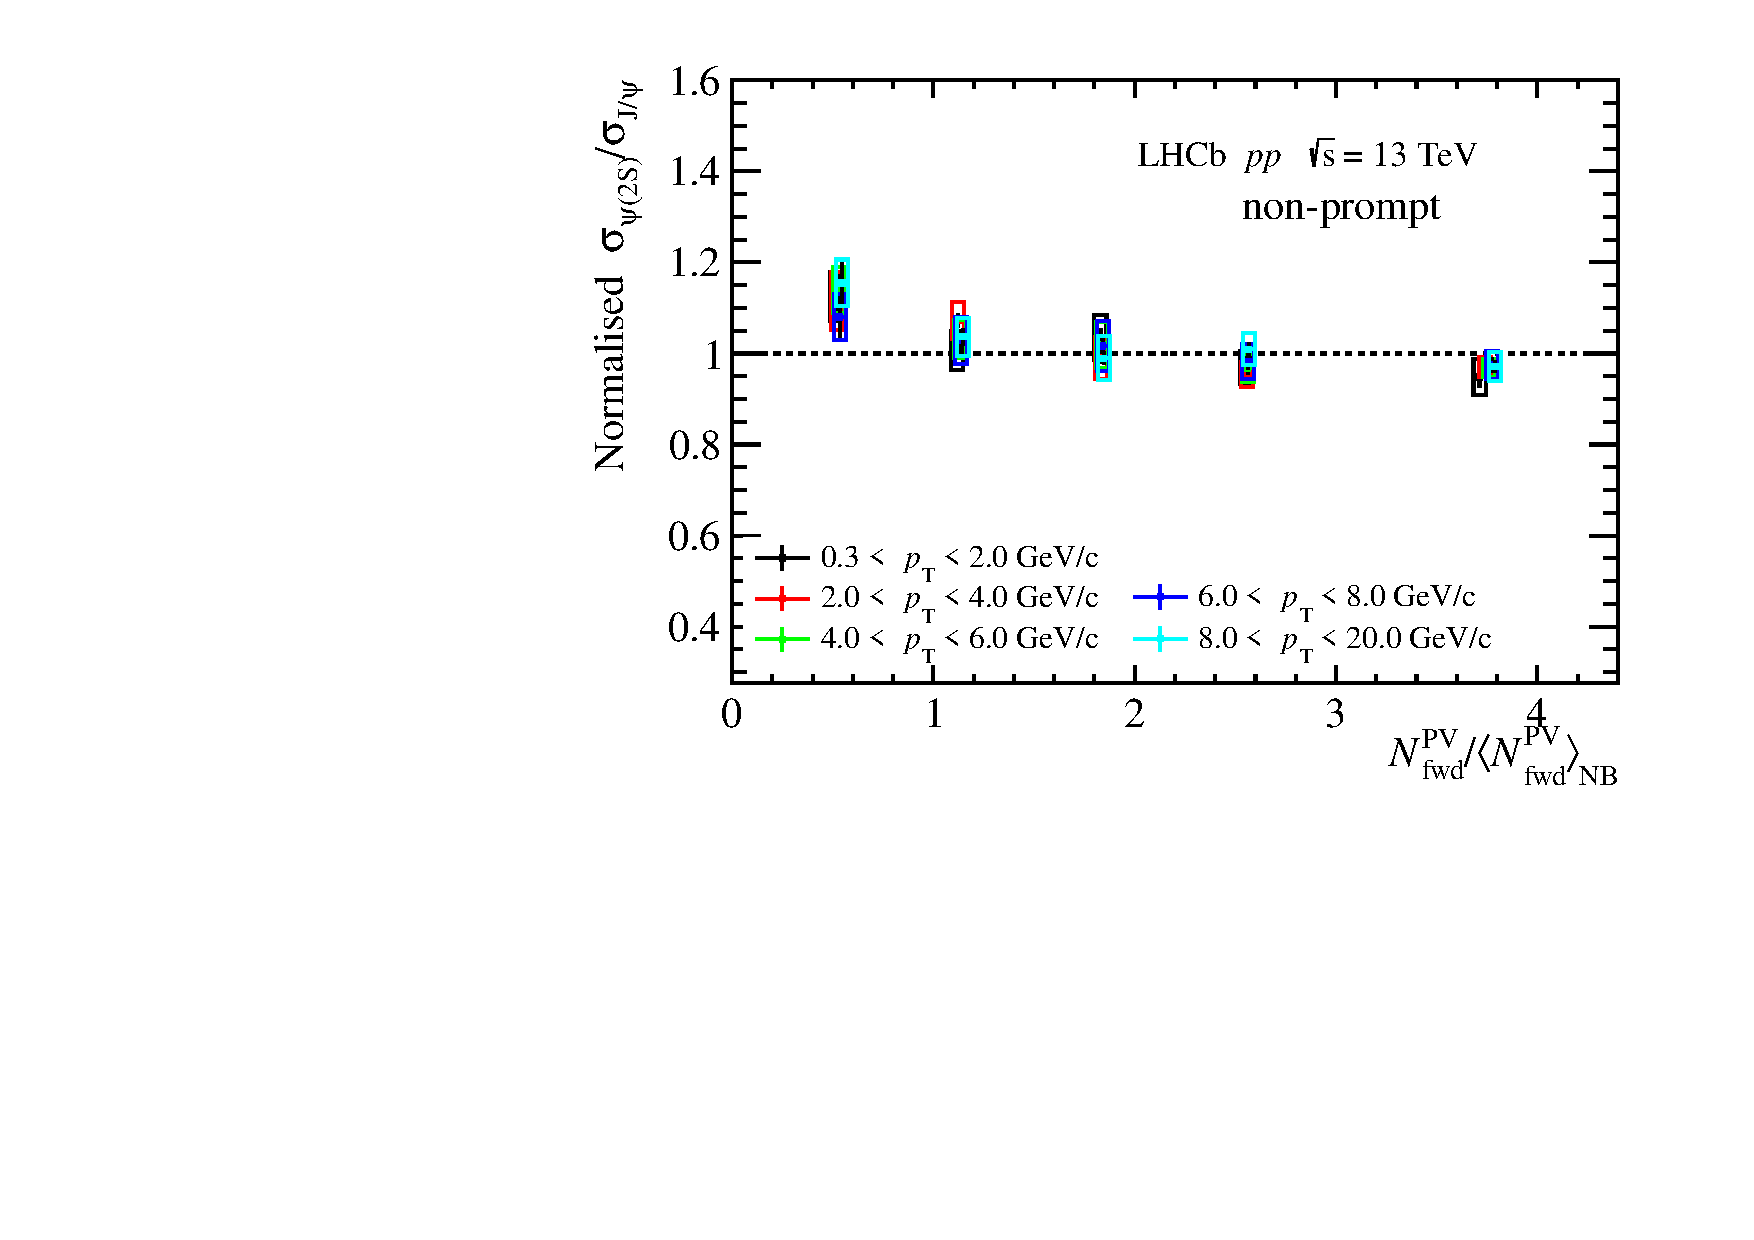
\includegraphics[width=0.48\linewidth]{pdf/Result/frombRatioPTF.pdf}
	  \vspace*{-0.5cm}
  \end{center}
	\caption{Normalised production ratio for (left) prompt and(right) non-prompt charmonia as a function of $N_{\rm fwd}^{\rm PV}/\langle N_{\rm fwd}^{\rm PV}\rangle_{\rm{NB}}$ in different \pt intervals.}
  \label{RatioPT_For}
\end{figure}
\begin{figure}[H]
  \begin{center}
	  \vspace*{-0.5cm}
    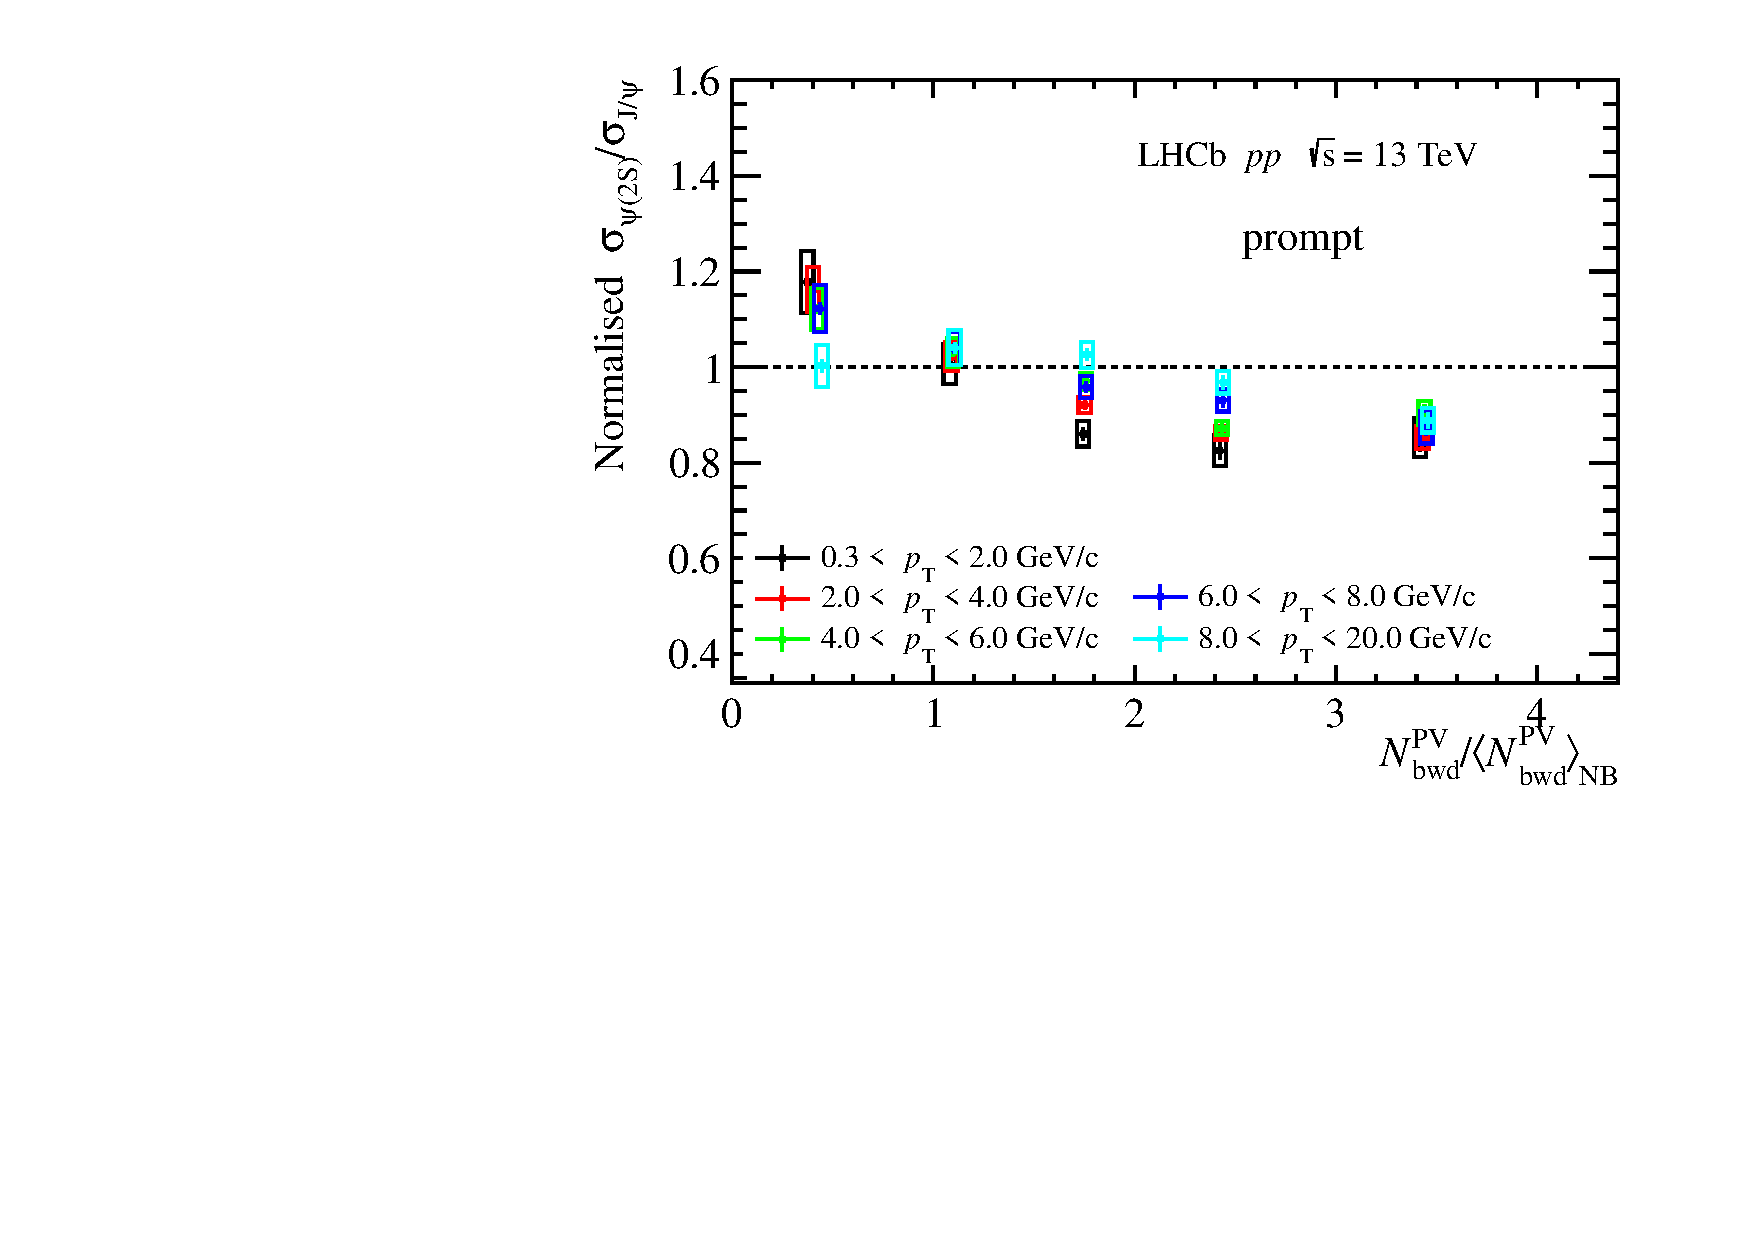
\includegraphics[width=0.48\linewidth]{pdf/Result/promptRatioPTB.pdf}
    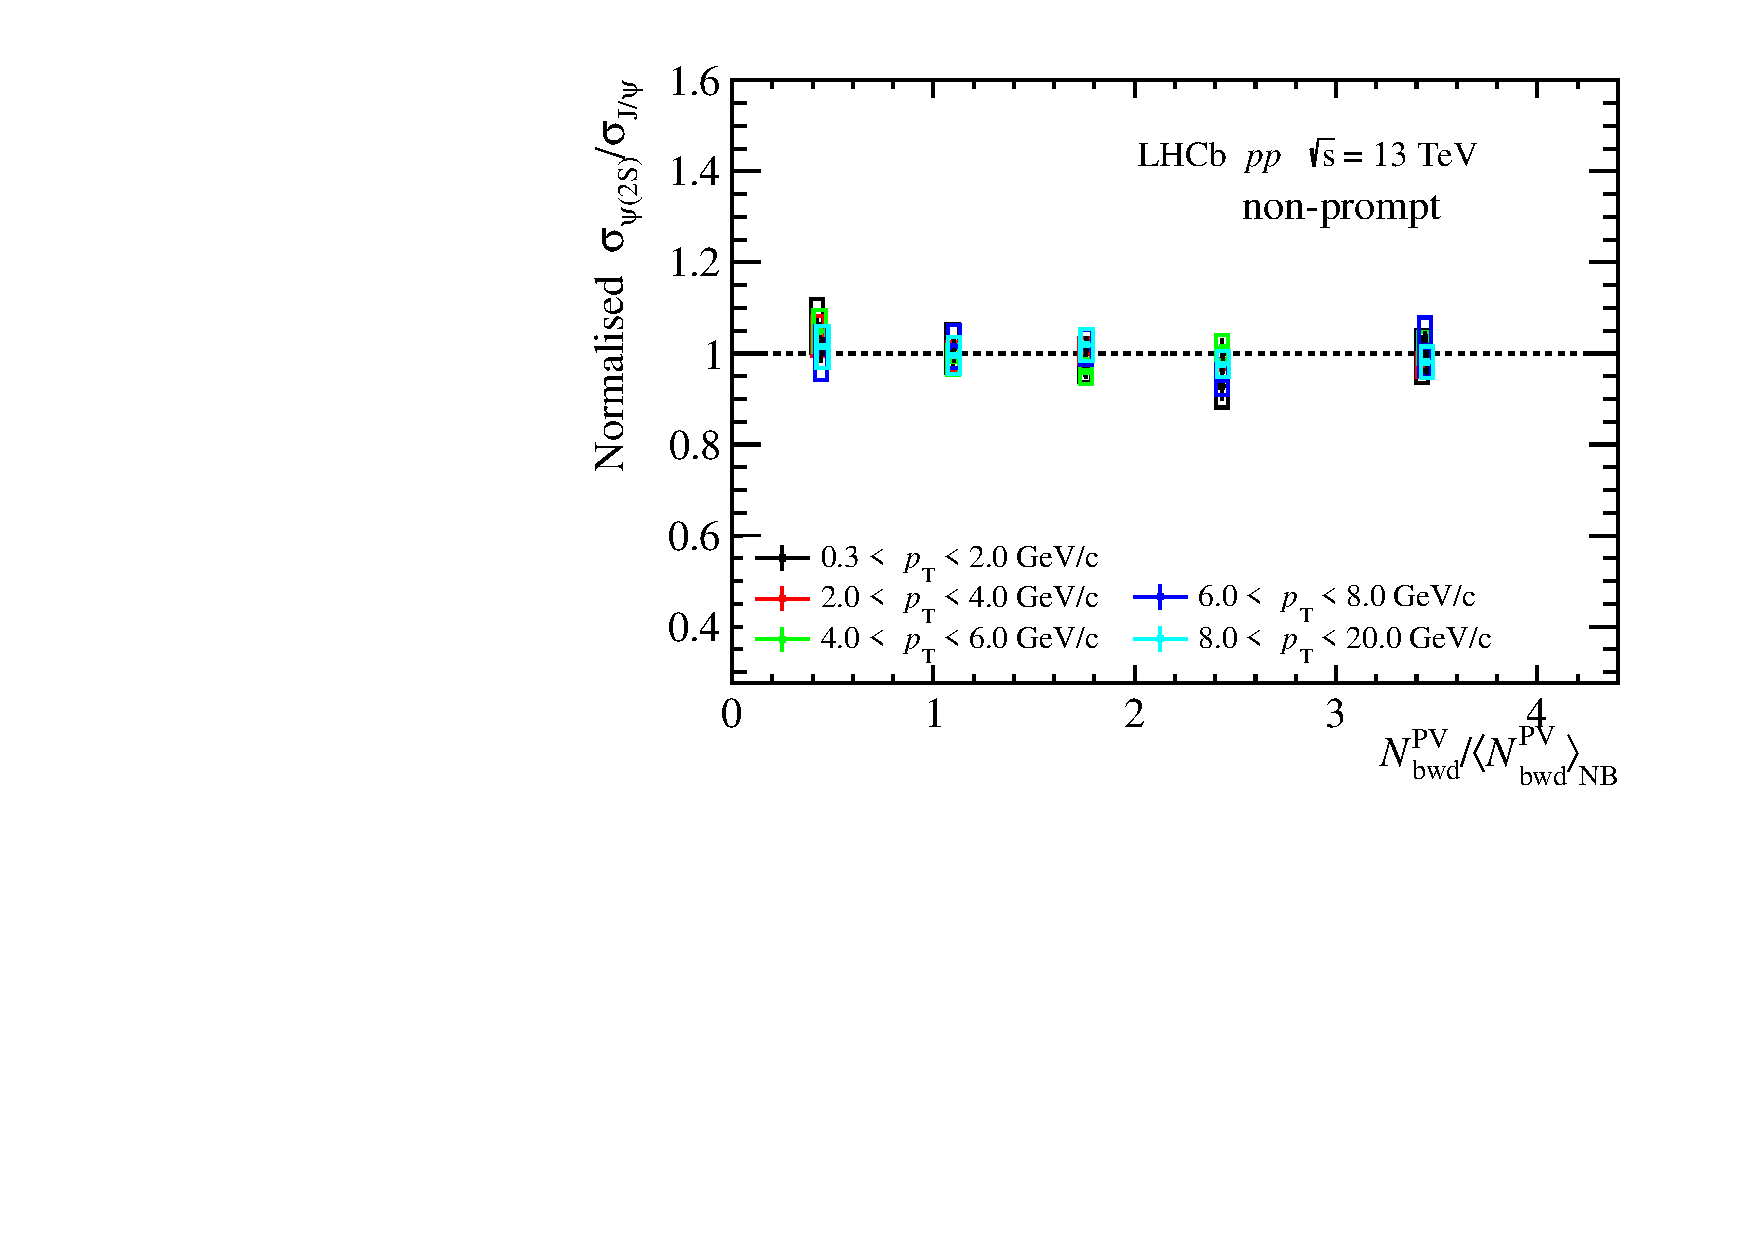
\includegraphics[width=0.48\linewidth]{pdf/Result/frombRatioPTB.pdf}
	  \vspace*{-0.5cm}
  \end{center}
	\caption{Normalised production ratio for (left) prompt and(right) non-prompt charmonia as a function of $N_{\rm bwd}^{\rm PV}/\langle N_{\rm bwd}^{\rm PV}\rangle_{\rm{NB}}$ in different \pt intervals.}
  \label{RatioPT_Back}
\end{figure}

The results for the ratio in different rapidity bins are shown in Figs.~\ref{RatioY},~\ref{RatioY_For} and~\ref{RatioY_Back}. Notably, there is minimal difference across different rapidity regions, for both prompt and non-prompt signals.

\begin{figure}[H]
  \begin{center}

    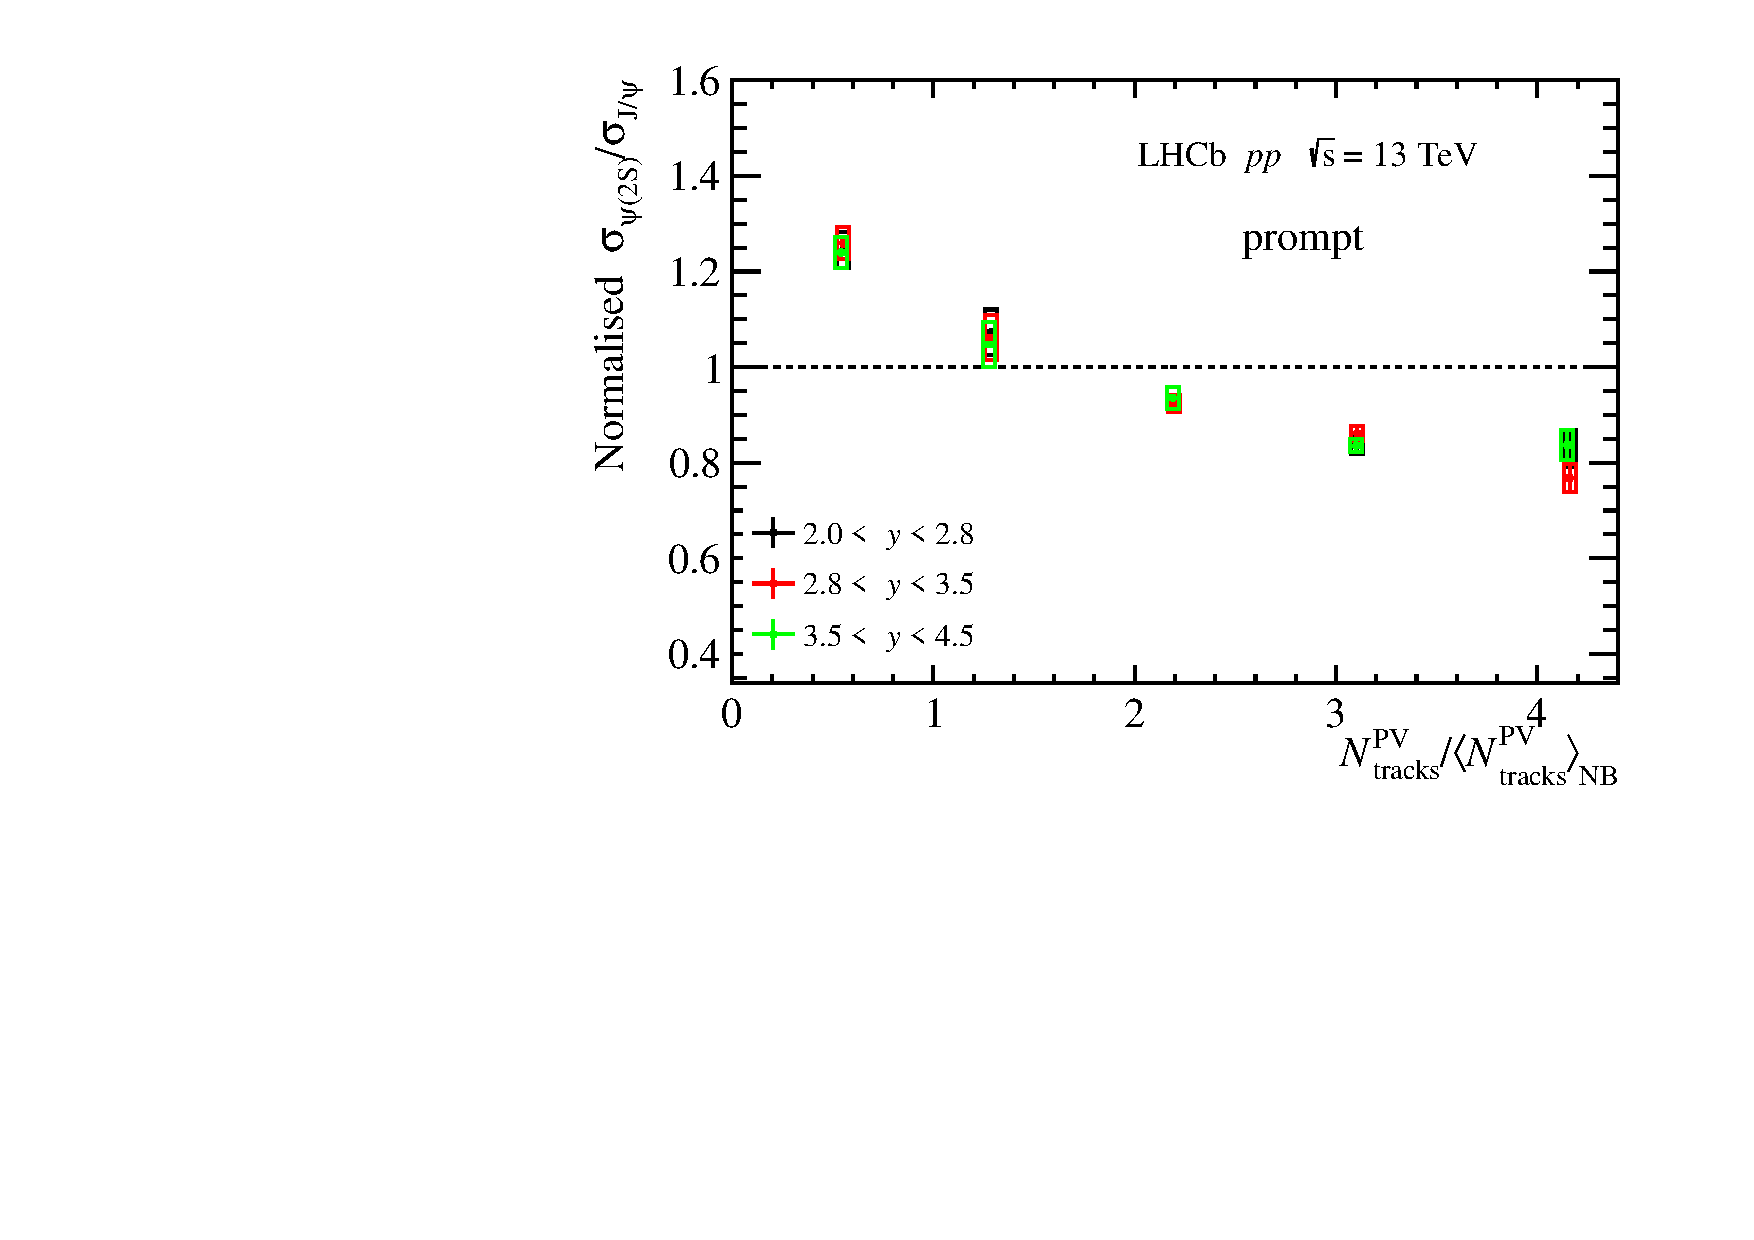
\includegraphics[width=0.48\linewidth]{pdf/Result/promptRatioY.pdf}
    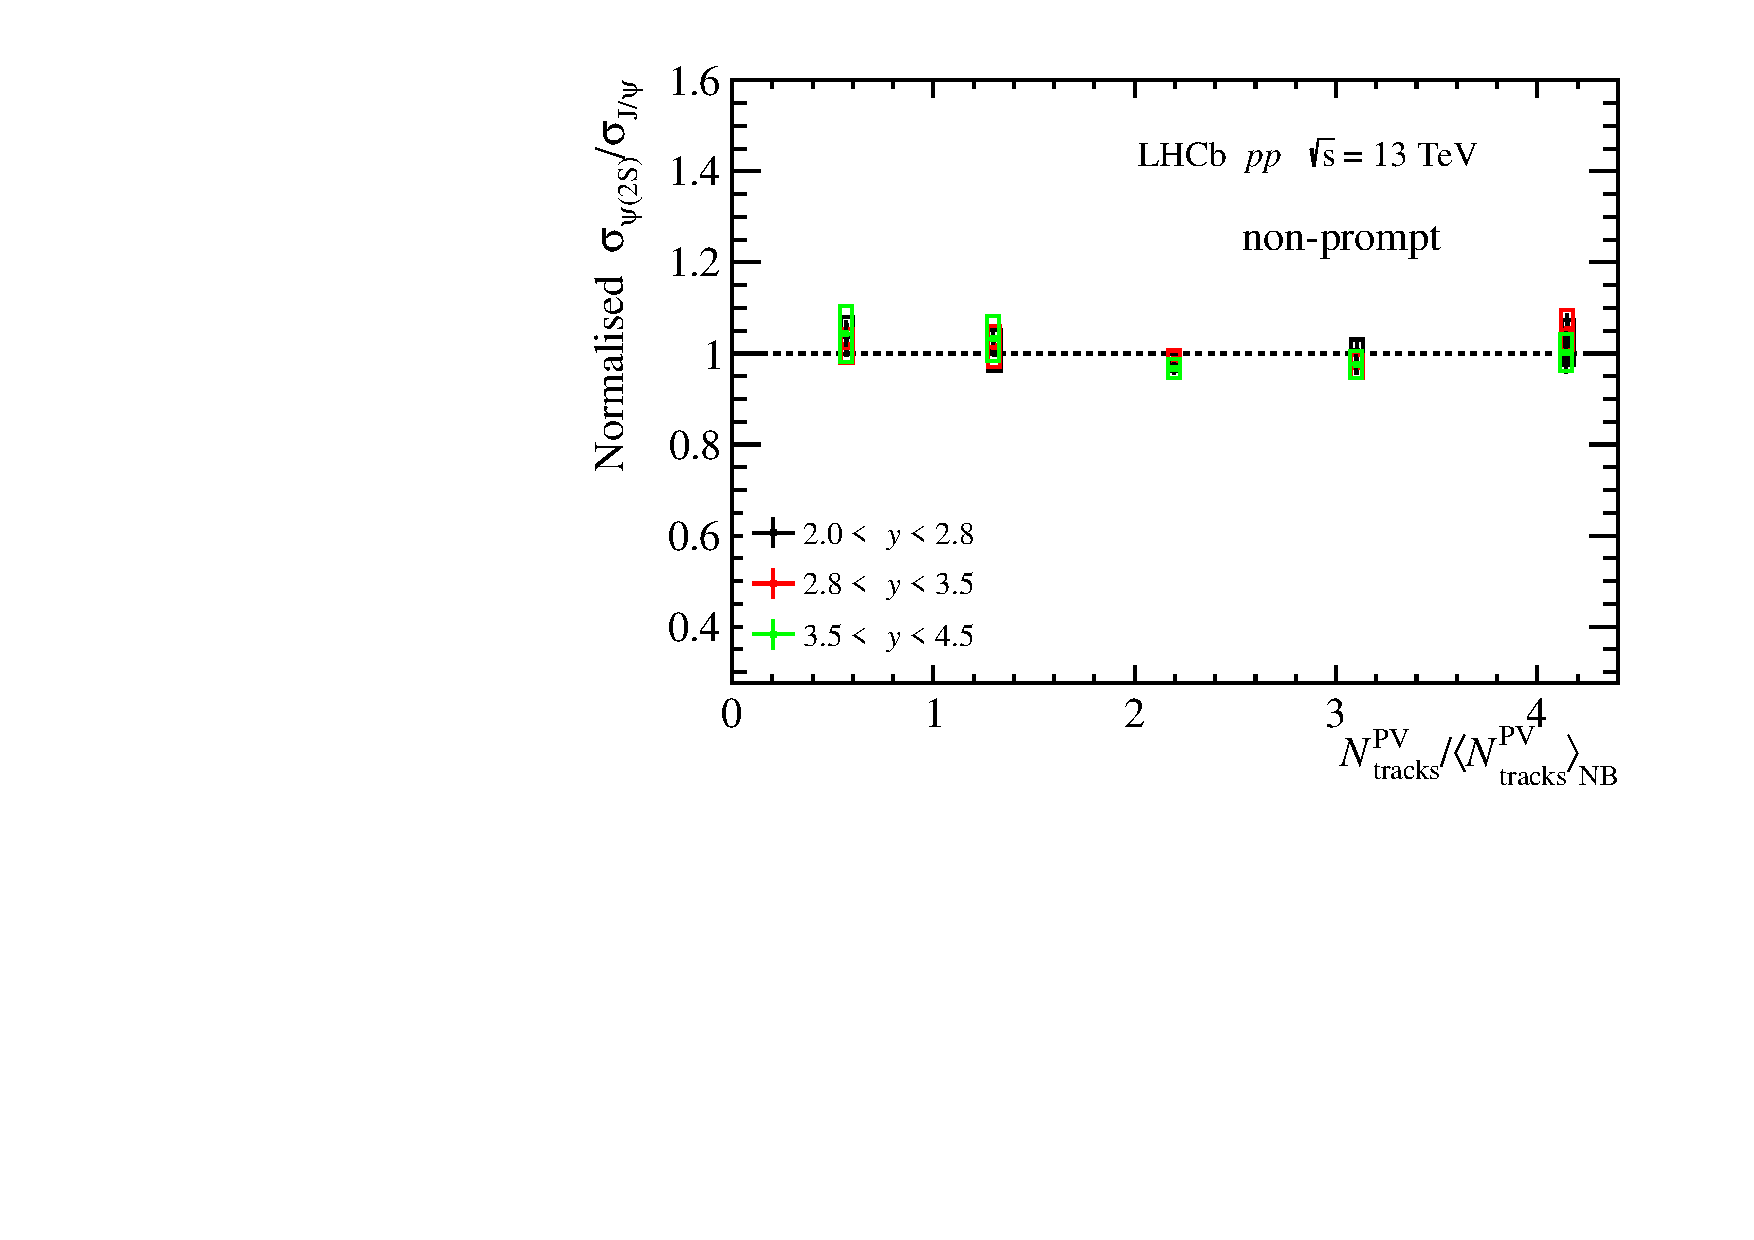
\includegraphics[width=0.48\linewidth]{pdf/Result/frombRatioY.pdf}
	  \vspace*{-0.5cm}
  \end{center}
	\caption{Normalised production ratio for (left) prompt and(right) non-prompt charmonia as a function of $N_{\rm tracks}^{\rm PV}/\langle N_{\rm tracks}^{\rm PV}\rangle_{\rm{NB}}$ in different $y$ intervals.}
  \label{RatioY}
\end{figure}

\begin{figure}[H]
  \begin{center}
	  \vspace*{-0.5cm}
    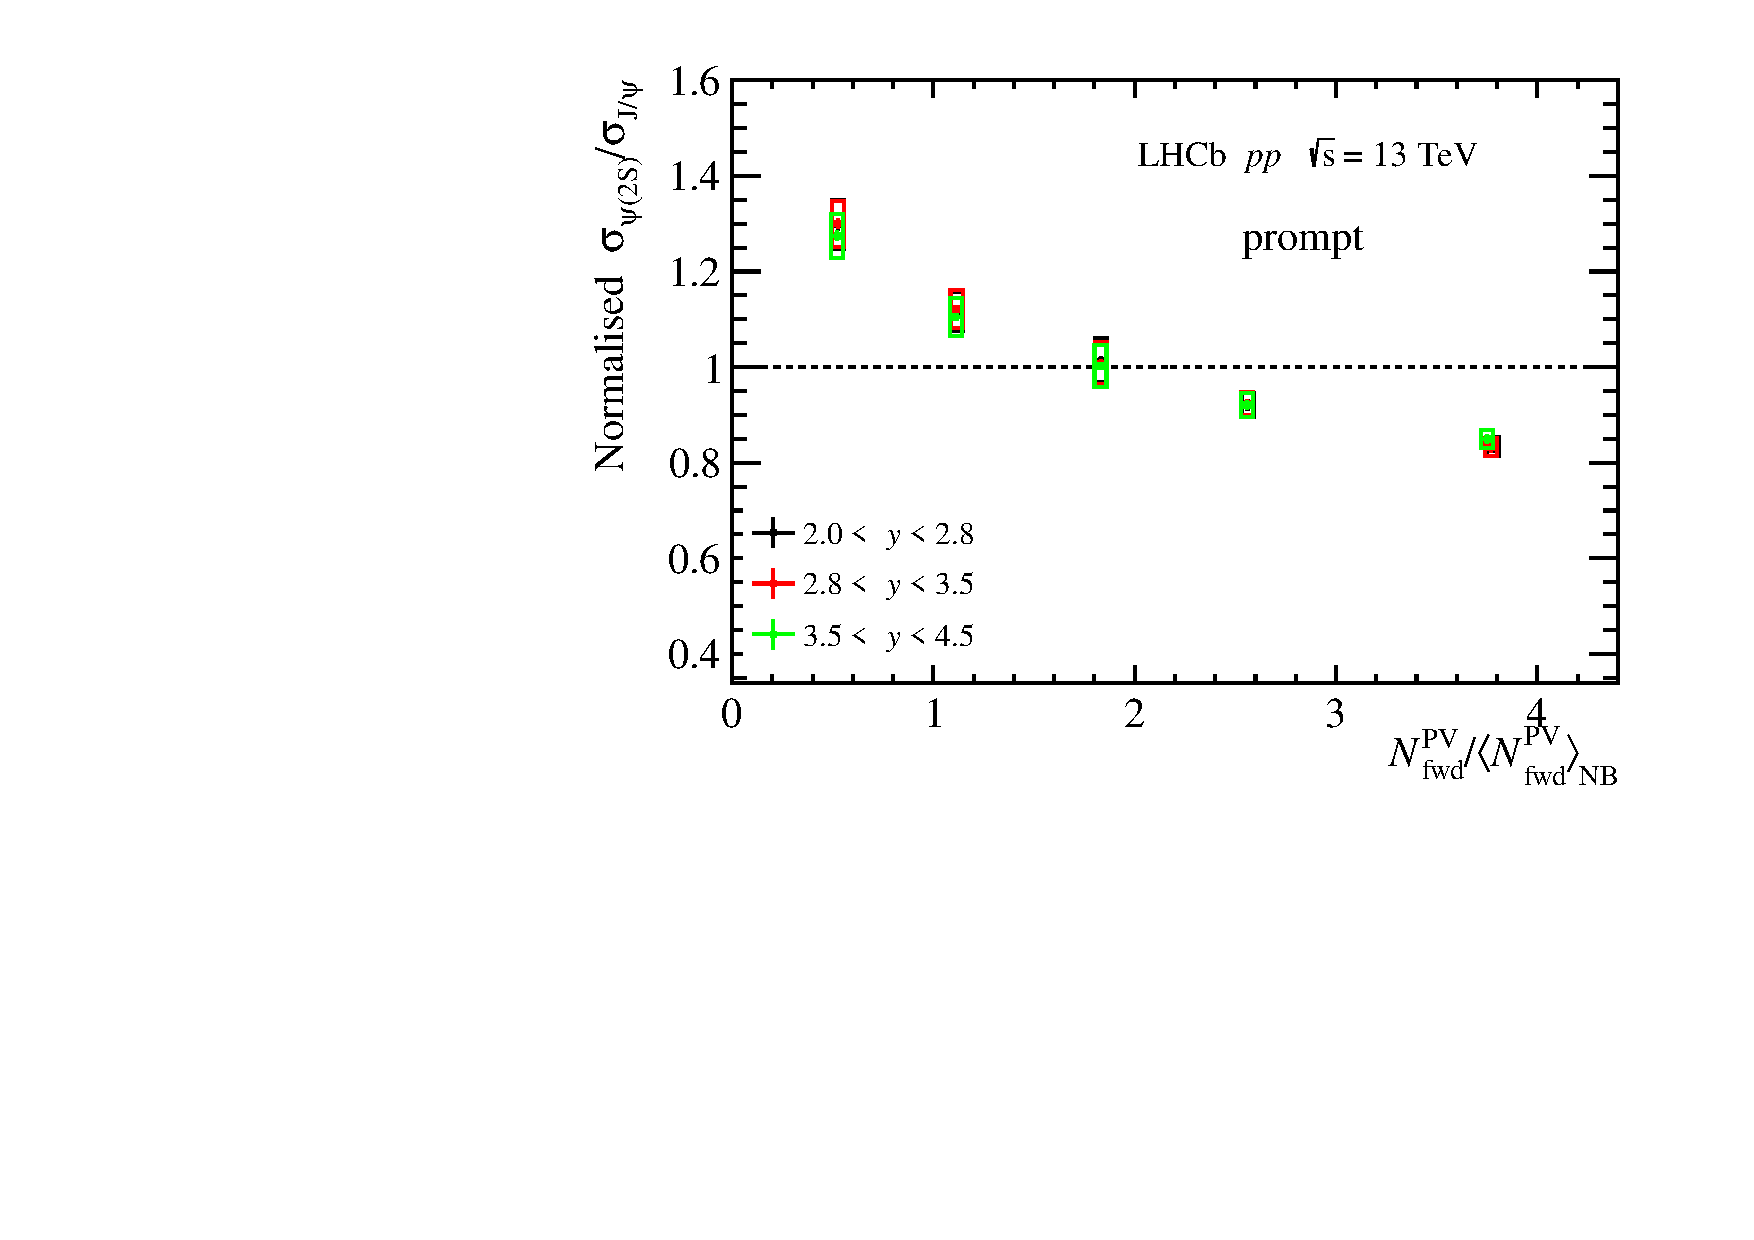
\includegraphics[width=0.48\linewidth]{pdf/Result/promptRatioYF.pdf}
    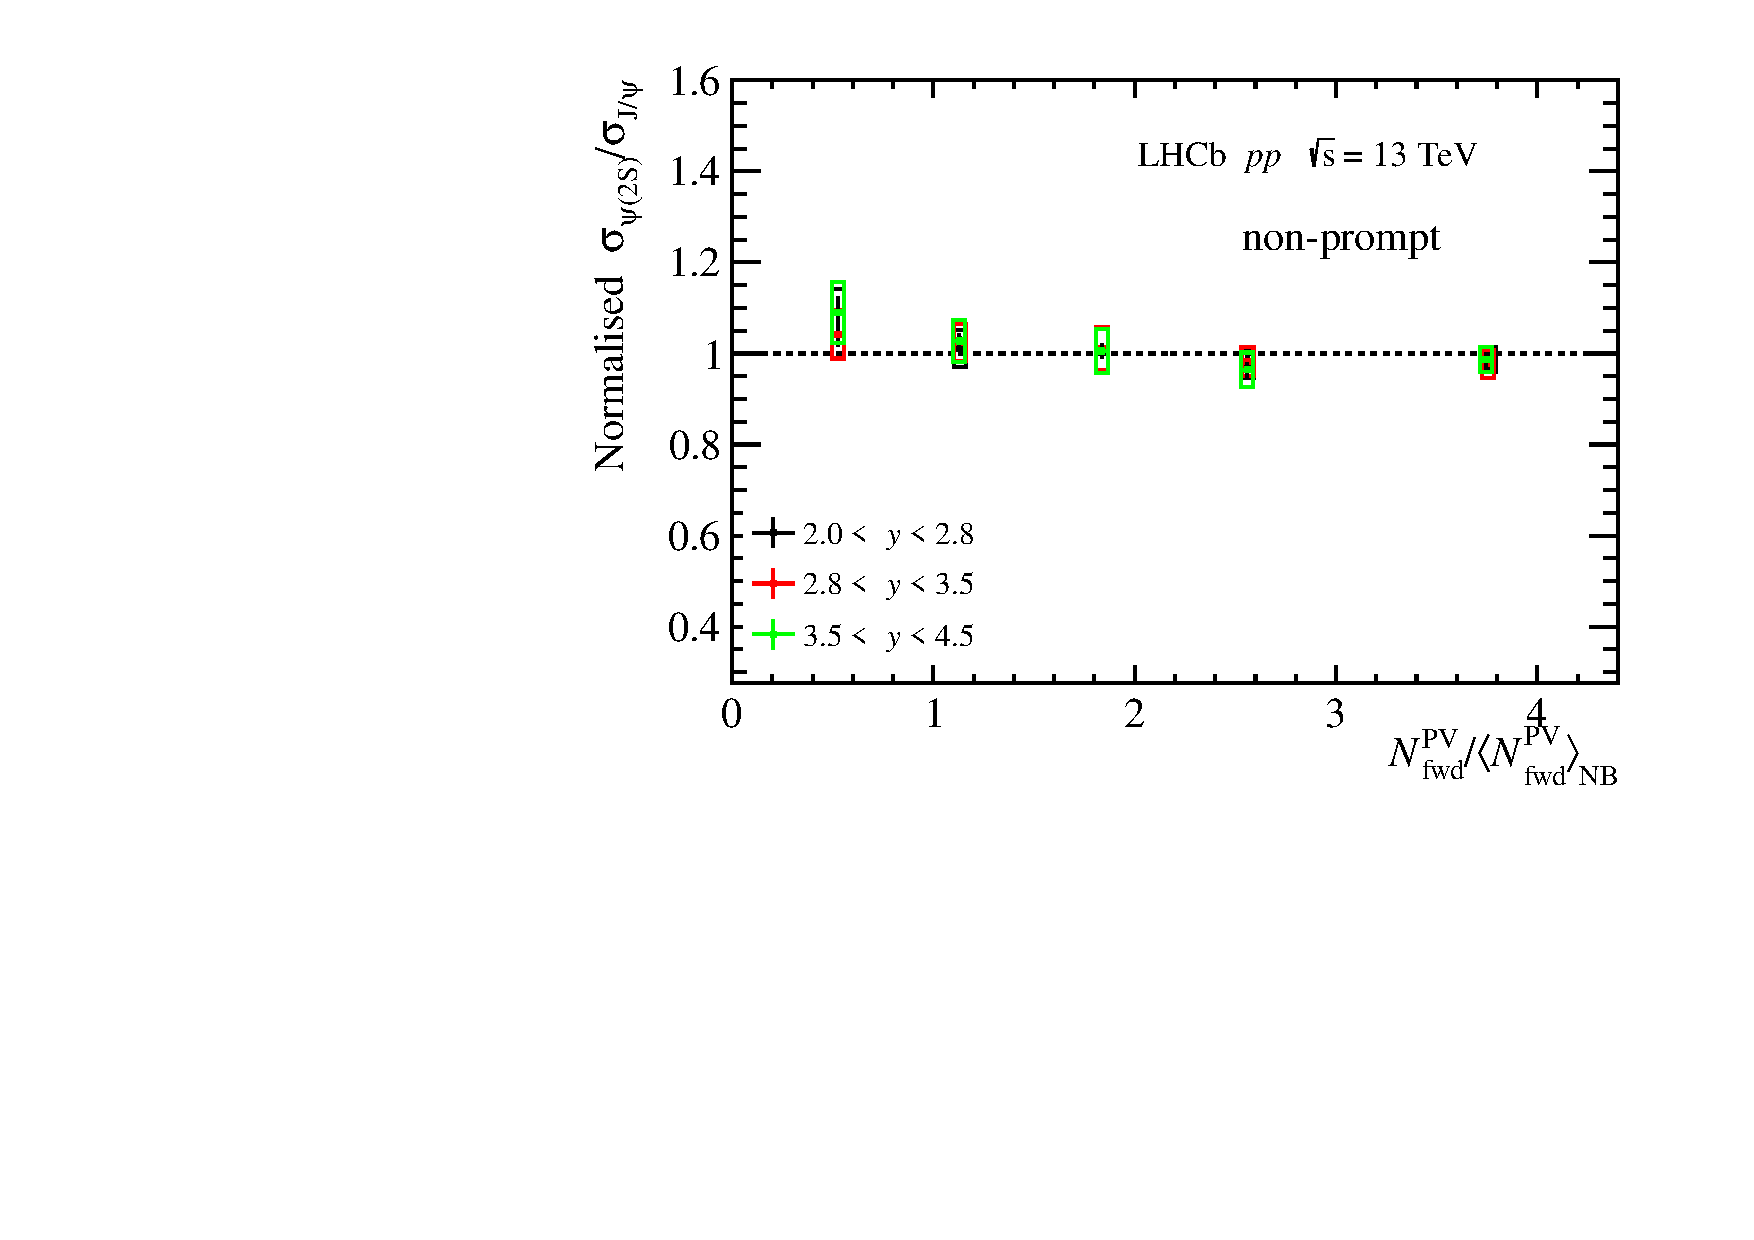
\includegraphics[width=0.48\linewidth]{pdf/Result/frombRatioYF.pdf}
	  \vspace*{-0.5cm}
  \end{center}
	\caption{Normalised production ratio for (left) prompt and(right) non-prompt charmonia as a function of $N_{\rm fwd}^{\rm PV}/\langle N_{\rm fwd}^{\rm PV}\rangle_{\rm{NB}}$ in different $y$ intervals.}
  \label{RatioY_For}
\end{figure}

\begin{figure}[H]
  \begin{center}
	  \vspace*{-0.5cm}
    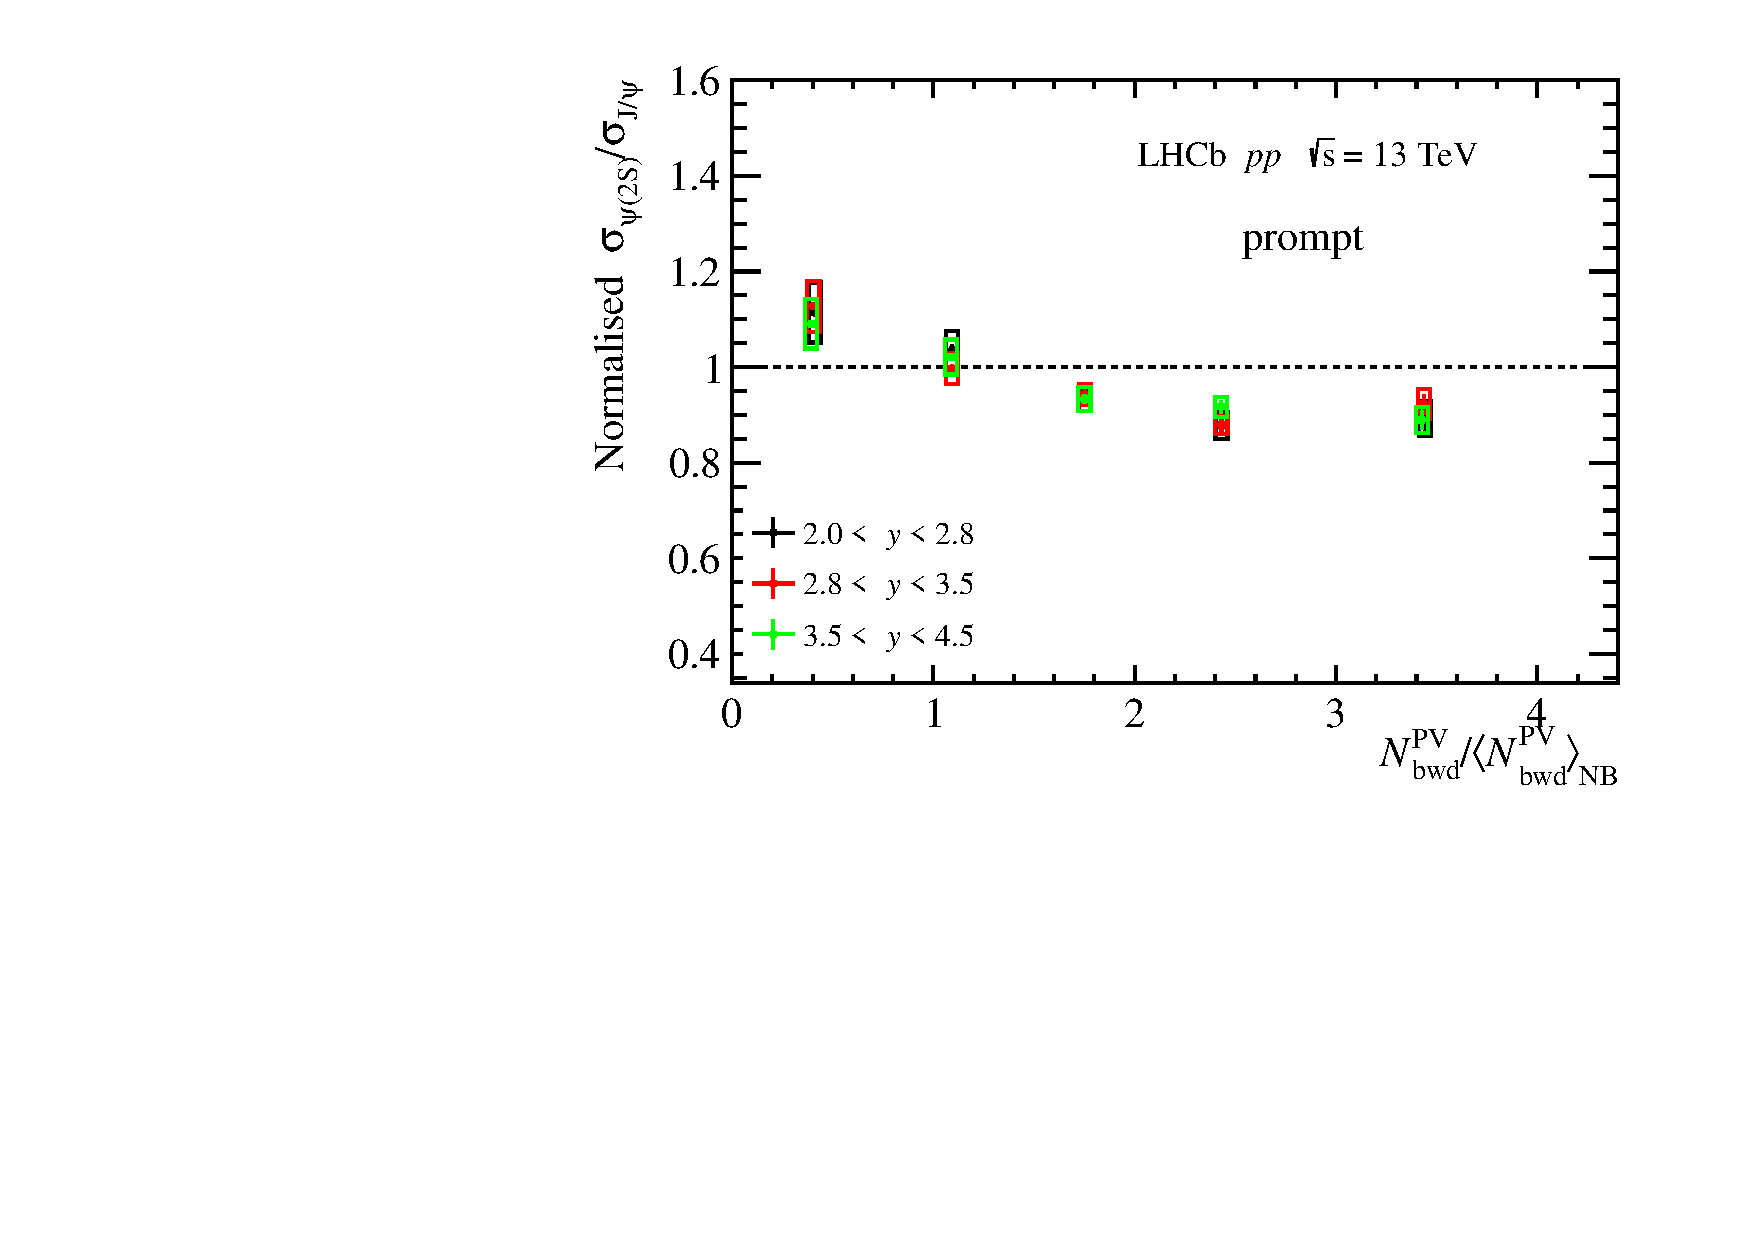
\includegraphics[width=0.48\linewidth]{pdf/Result/promptRatioYB.pdf}
    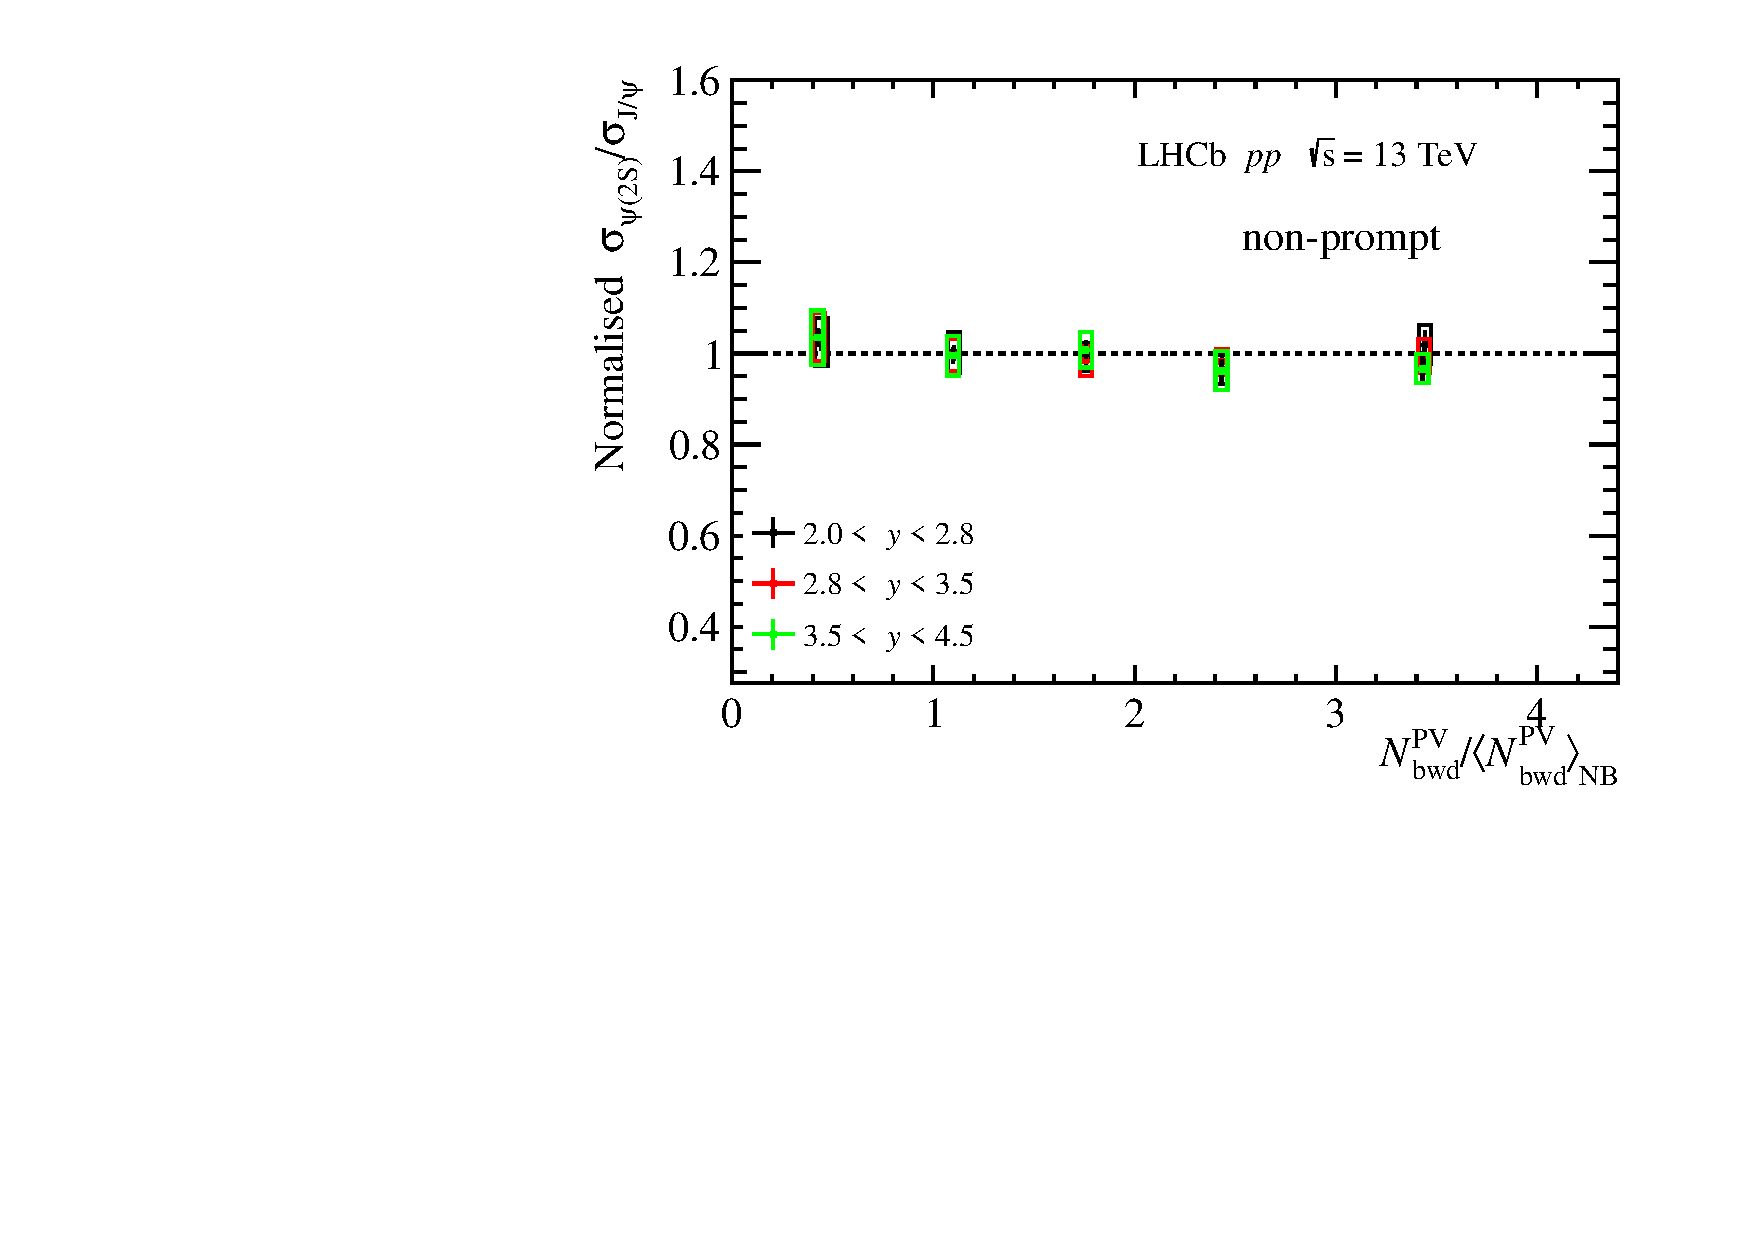
\includegraphics[width=0.48\linewidth]{pdf/Result/frombRatioYB.pdf}
	  \vspace*{-0.5cm}
  \end{center}
	\caption{Normalised production ratio for (left) prompt and(right) non-prompt charmonia as a function of $N_{\rm bwd}^{\rm PV}/\langle N_{\rm bwd}^{\rm PV}\rangle_{\rm{NB}}$ in different $y$ intervals.}
  \label{RatioY_Back}
\end{figure}

\subsection{Comparisons with other measurements}
\label{Compare}
Measurements of $\BR_{\psitwos}\times\sigma_{\psitwos}$ with $\BR_{\jpsi}\times\sigma_{\jpsi}$ have been carried out across diverse collision systems and energies by comparing the ratio of $\sigma_{\psitwos}/\sigma_{\jpsi}$ alongside their branching fractions and systematic uncertainties. Remarkably, the ratio is consistent regardless of the collision systems and energies. A comprehensive comparison is shown in Figs.~\ref{compare_total} and~\ref{compare_pt}, revealing strong agreement with other measurements~\cite{PHENIX:2016vmz,NA50:2006rdp,PHENIX:2011gyb,E705:1992vec,NA51:1998uun,Clark:1978mg,UA1:1990eni,CDF:1997ykw,LHCb:2013nqs,CMS:2011rxs,ALICE:2017leg}, which has been summarized in~\cite{PHENIX:2016vmz}. The value of this measurement is
\begin{equation}
		\frac{\BR_{\psitwos}\times\sigma_{\psitwos}}{\BR_{\jpsi}\times\sigma_{\jpsi}} = (1.894\pm0.039)\%.
\end{equation}

\begin{figure}[H]
  \begin{center}
  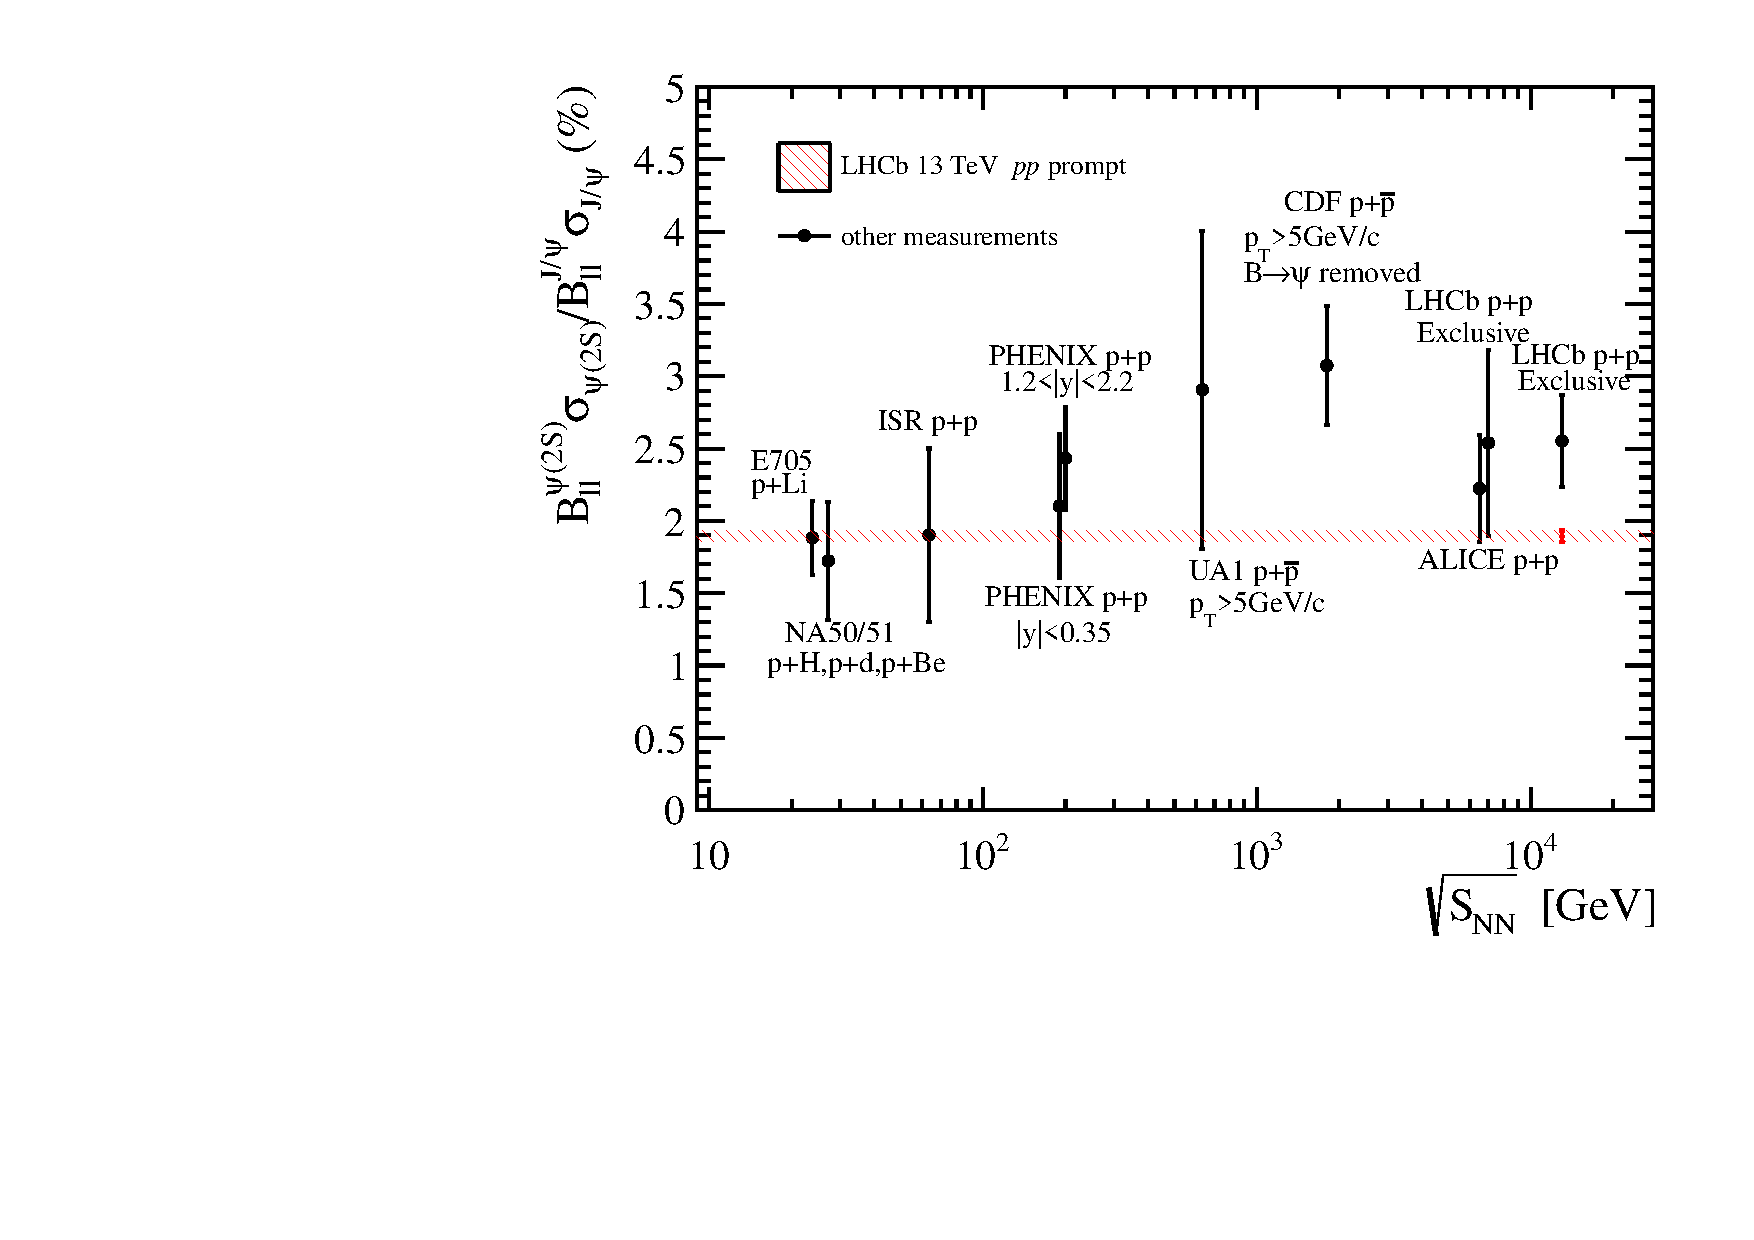
\includegraphics[width=0.7\linewidth]{pdf/Result/VariousMeasurements.pdf }
  \end{center}
  \caption{Production ratios compared to existing measurements~\cite{PHENIX:2016vmz}.}
\label{compare_total}
\end{figure}
\begin{figure}[H]
  \begin{center}
  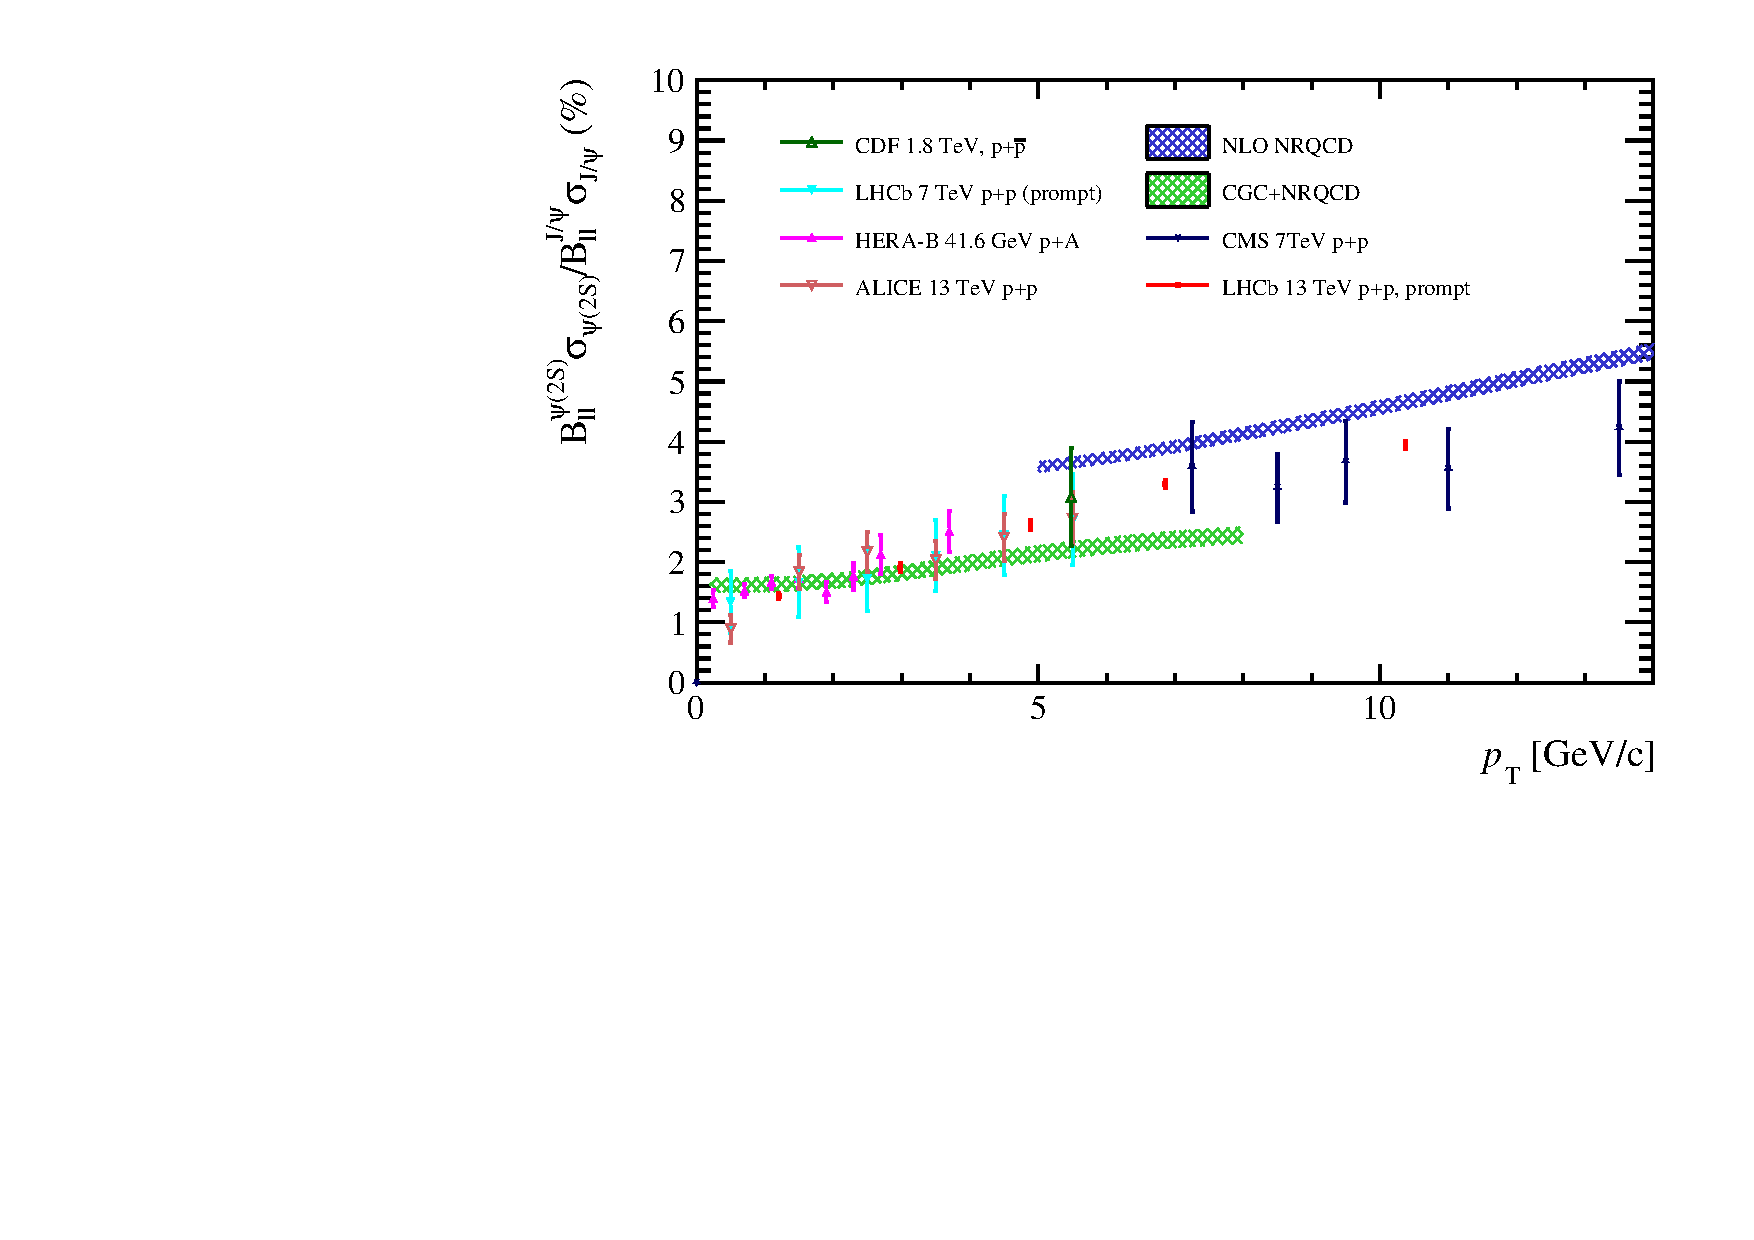
\includegraphics[width=0.7\linewidth]{pdf/Result/Comparisons_PT_VariousMeasurements.pdf}
  \end{center}
  \caption{Production ratios as a function of \pt compared to existing measurements~\cite{PHENIX:2016vmz} and model predictions~\cite{Ma:2014mri}.}
\label{compare_pt}
\end{figure}



%Conclusion:
\cleardoublepage
\section{Conclusion}
\label{sec:conclusion}

This analysis presents a measurement of the the normalised \psitwos-to-\jpsi cross-section ratio, as a function of different charged-track multiplicity variables, in $pp$ collisions at $\sqrt{s}=13$~TeV. The data sample was collected by the \lhcb detector in 2016 and corresponds to an integrated luminosity of $658\pm 13$\invpb.

Notably, for non-prompt production the cross-section ratio exhibits no dependence on any of these multiplicity variables. In contrast, in prompt production the ratio decreases as a function of $N_{\rm tracks}^{\rm PV}$, which is a trend that aligns well with the predictions of the co-mover model. Furthermore, the ratio for prompt production has a similar trend as a function of $N_{\rm fwd}^{\rm PV}$, which can be attributed to the correlation between the multiplicity and the charmonium production, a phenomenon that can also be ascribed to the co-mover effect. The use of $N_{\rm bwd}^{\rm PV}$ serves to mitigate this correlation, leading to a small yet observable diminishing trend in relation to multiplicity. The small dependence on $N_{\rm bwd}^{\rm PV}$ could arise from the correlation between $N_{\rm bwd}^{\rm PV}$ and $N_{\rm fwd}^{\rm PV}$. The distinct behaviors exhibited by the prompt and non-prompt components underscore the significant influence of interactions with other particles within the collision event on charmonium production, even in $pp$ collisions. Furthermore, the variation of these ratios as a function of different multiplicity variables further solidifies this perspective. 

The multiplicity dependence of the ratios is also measured in distinct \pt and $y$ regions, uncovering an enhanced suppression pattern at low \pt, and an almost multiplicity independence in the high-\pt region for prompt \psitwos-to-\jpsi ratio, regardless of the choice of multiplicity variables. Finally, the results of the ratio $\BR_{\psitwos} \times \sigma_{\psitwos}$ over $\BR_{\jpsi} \times \sigma_{\jpsi}$ are compared with other measurements, and are found to be in agreement with a relative higher precision.


%Acknowledgements:
\section*{Acknowledgements}
%
% These Acknowledgements valid from 3-May-2019
%
We express our gratitute to Elena Gonzalez Ferreiro for the co-mover model predictions and YanQing Ma for the NRQCD model predictions.
We express our gratitude to our colleagues in the CERN
accelerator departments for the excellent performance of the LHC. We
thank the technical and administrative staff at the LHCb
institutes.
We acknowledge support from CERN and from the national agencies:
CAPES, CNPq, FAPERJ and FINEP (Brazil); 
MOST and NSFC (China); 
CNRS/IN2P3 (France); 
BMBF, DFG and MPG (Germany); 
INFN (Italy); 
NWO (Netherlands); 
MNiSW and NCN (Poland); 
MCID/IFA (Romania); 
%MSHE (Russia); 
MICINN (Spain); 
SNSF and SER (Switzerland); 
NASU (Ukraine); 
STFC (United Kingdom); 
DOE NP and NSF (USA).
We acknowledge the computing resources that are provided by CERN, IN2P3
(France), KIT and DESY (Germany), INFN (Italy), SURF (Netherlands),
PIC (Spain), GridPP (United Kingdom), 
%RRCKI and Yandex LLC (Russia), 
CSCS (Switzerland), IFIN-HH (Romania), CBPF (Brazil),
and Polish WLCG (Poland).
We are indebted to the communities behind the multiple open-source
software packages on which we depend.
Individual groups or members have received support from
ARC and ARDC (Australia);
Key Research Program of Frontier Sciences of CAS, CAS PIFI, CAS CCEPP, 
Fundamental Research Funds for the Central Universities, 
and Sci. \& Tech. Program of Guangzhou (China);
Minciencias (Colombia);
EPLANET, Marie Sk\l{}odowska-Curie Actions, ERC and NextGenerationEU (European Union);
A*MIDEX, ANR, IPhU and Labex P2IO, and R\'{e}gion Auvergne-Rh\^{o}ne-Alpes (France);
%RFBR, RSF and Yandex LLC (Russia);
AvH Foundation (Germany);
ICSC (Italy); 
GVA, XuntaGal, GENCAT, Inditex, InTalent and Prog.~Atracci\'on Talento, CM (Spain);
SRC (Sweden);
the Leverhulme Trust, the Royal Society
 and UKRI (United Kingdom).

 %Appendix
\clearpage
\section*{A. Numeric results}
\label{Sec:Ratio}
%\subsection*{A.1 Taking $N^{PV}_{tracks}$ as multiplicity variable} 
\begin{table}[H]
    \centering
    \caption{Summary of systematic relative uncertainties of ratio of integrated production due to the uncertainty of trigger requirement for PVNTRACKS from 0 to 20.}
\begin{center}
    \begin{tabular}{ c | c | c }
        \hline
        Region & prompt (\%) & from $b$ (\%)\\
        \hline
        2.0$<$y$<$2.8&2.83&2.75\\
        2.8$<$y$<$3.5&2.81&2.80\\
        3.5$<$y$<$4.5&2.80&2.83\\
        \hline
        0\gevc $<$\pt$<$2\gevc&2.70&2.70\\
        2\gevc $<$\pt$<$4\gevc&2.70&2.70\\
        4\gevc $<$\pt$<$6\gevc&3.58&3.58\\
        6\gevc $<$\pt$<$8\gevc&1.02&1.02\\
        8\gevc $<$\pt$<$20\gevc&0.24&0.24\\
        \hline
        all \pt-y region&2.82&2.80\\
        \hline
    \end{tabular}
\end{center}
\label{input label here}
\end{table}

\begin{table}[H]
    \centering
    \caption{Summary of systematic relative uncertainties of ratio of integrated production due to the uncertainty of statistical uncertainty for PVNTRACKS from 20 to 40.}
\begin{center}
    \begin{tabular}{ c | c | c }
        \hline
        Region & prompt (\%) & from $b$ (\%)\\
        \hline
        2.0$<$y$<$2.8&0.90&1.44\\
        2.8$<$y$<$3.5&0.71&1.24\\
        3.5$<$y$<$4.5&0.65&1.46\\
        \hline
        0\gevc $<$\pt$<$2\gevc&0.87&1.82\\
        2\gevc $<$\pt$<$4\gevc&0.73&1.29\\
        4\gevc $<$\pt$<$6\gevc&0.73&1.34\\
        6\gevc $<$\pt$<$8\gevc&0.94&1.64\\
        8\gevc $<$\pt$<$20\gevc&1.09&1.52\\
        \hline
        all \pt-y region&0.46&0.82\\
        \hline
    \end{tabular}
\end{center}
\label{input label here}
\end{table}

\begin{table}[H]
    \centering
    \caption{Summary of systematic relative uncertainties of ratio of integrated production due to the uncertainty of statistical uncertainty for PVNTRACKS from 40 to 60.}
\begin{center}
    \begin{tabular}{ c | c | c }
        \hline
        Region & prompt (\%) & from $b$ (\%)\\
        \hline
        2.0$<$y$<$2.8&1.43&1.51\\
        2.8$<$y$<$3.5&1.11&1.26\\
        3.5$<$y$<$4.5&0.92&1.55\\
        \hline
        0\gevc $<$\pt$<$2\gevc&1.67&2.06\\
        2\gevc $<$\pt$<$4\gevc&1.08&1.37\\
        4\gevc $<$\pt$<$6\gevc&0.90&1.31\\
        6\gevc $<$\pt$<$8\gevc&0.97&1.52\\
        8\gevc $<$\pt$<$20\gevc&0.97&1.34\\
        \hline
        all \pt-y region&0.71&0.86\\
        \hline
    \end{tabular}
\end{center}
\label{input label here}
\end{table}

\begin{table}[H]
    \centering
    \caption{Summary of systematic relative uncertainties of ratio of integrated production due to the uncertainty of trigger requirement for PVNTRACKS from 60 to 80.}
\begin{center}
    \begin{tabular}{ c | c | c }
        \hline
        Region & prompt (\%) & from $b$ (\%)\\
        \hline
        2.0$<$y$<$2.8&-1.38&-1.41\\
        2.8$<$y$<$3.5&-1.37&-1.48\\
        3.5$<$y$<$4.5&-1.52&-1.62\\
        \hline
        0\gevc $<$\pt$<$2\gevc&-3.21&-3.21\\
        2\gevc $<$\pt$<$4\gevc&-2.88&-2.88\\
        4\gevc $<$\pt$<$6\gevc&1.54&1.54\\
        6\gevc $<$\pt$<$8\gevc&-1.18&-1.18\\
        8\gevc $<$\pt$<$20\gevc&-1.26&-1.26\\
        \hline
        all \pt-y region&2.14&-3.41\\
        \hline
    \end{tabular}
\end{center}
\label{input label here}
\end{table}

\begin{table}[H]
    \centering
    \caption{Summary of systematic relative uncertainties of ratio of integrated production due to the uncertainty of statistical uncertainty for PVNTRACKS from 80 to 200.}
\begin{center}
    \begin{tabular}{ c | c | c }
        \hline
        Region & prompt (\%) & from $b$ (\%)\\
        \hline
        2.0$<$y$<$2.8&4.66&2.64\\
        2.8$<$y$<$3.5&3.13&2.33\\
        3.5$<$y$<$4.5&2.64&2.71\\
        \hline
        0\gevc $<$\pt$<$2\gevc&6.57&4.00\\
        2\gevc $<$\pt$<$4\gevc&3.37&2.38\\
        4\gevc $<$\pt$<$6\gevc&2.20&2.16\\
        6\gevc $<$\pt$<$8\gevc&1.89&2.43\\
        8\gevc $<$\pt$<$20\gevc&1.51&1.98\\
        \hline
        all \pt-y region&2.25&1.54\\
        \hline
    \end{tabular}
\end{center}
\label{input label here}
\end{table}

%\subsection*{A.2 Taking $N^{PV}_bwd$ as multiplicity variable} 
\begin{table}[H]
\caption{Ratio(\%) of double differential production cross-section for prompt \psitwos to \jpsi in bins of (\pt,$y$). The first uncertainties are statistical, the second are the systematic uncertainties, for 0 $\leq$ nBackTracks $<$ 8. }
\centering
\resizebox{\linewidth}{!}{
\begin{tabular}{|c|ccc|}
\hline
\multicolumn{4}{|c|}{prompt}\\\hline
\pt(\gevc)& $2<y<2.8$& $2.8<y<3.5$& $3.5<y<4.5$ \\
\hline
0-2&$12.78\pm0.18\pm0.89$&$12.48\pm0.14\pm0.66$&$12.88\pm0.13\pm0.75$\\
2-4&$17.26\pm0.23\pm0.81$&$16.40\pm0.18\pm0.68$&$16.36\pm0.18\pm0.66$\\
4-6&$23.45\pm0.36\pm1.07$&$21.17\pm0.26\pm0.87$&$20.84\pm0.29\pm0.88$\\
6-8&$30.78\pm0.62\pm1.63$&$26.87\pm0.47\pm1.26$&$26.21\pm0.53\pm1.31$\\
8-20&$32.25\pm0.71\pm1.68$&$28.28\pm0.60\pm1.42$&$27.93\pm0.76\pm1.46$\\
\hline
\multicolumn{4}{|c|}{from $b$}\\\hline
\pt(\gevc)& $2<y<2.8$& $2.8<y<3.5$& $3.5<y<4.5$ \\
\hline
0-2&$21.71\pm0.88\pm2.39$&$20.83\pm0.72\pm1.38$&$21.28\pm0.82\pm1.67$\\
2-4&$26.41\pm0.79\pm1.31$&$26.46\pm0.63\pm1.29$&$26.41\pm0.75\pm1.35$\\
4-6&$34.65\pm1.00\pm1.70$&$29.13\pm0.71\pm1.39$&$30.13\pm0.95\pm1.69$\\
6-8&$33.39\pm1.23\pm2.17$&$31.37\pm1.02\pm1.85$&$33.99\pm1.40\pm2.61$\\
8-20&$41.81\pm1.26\pm2.03$&$36.94\pm1.11\pm2.00$&$35.45\pm1.45\pm2.12$\\
\hline
\end{tabular}
}
\label{RatioBACK1}
\end{table}

\begin{table}[H]
\caption{Ratio(\%) of double differential production cross-section for prompt \psitwos to \jpsi in bins of (\pt,$y$). The first uncertainties are statistical, the second are the systematic uncertainties, for 8 $\leq$ nBackTracks $<$ 15. }
\centering
\resizebox{\linewidth}{!}{
\begin{tabular}{|c|ccc|}
\hline
\multicolumn{4}{|c|}{prompt}\\\hline
\pt(\gevc)& $2<y<2.8$& $2.8<y<3.5$& $3.5<y<4.5$ \\
\hline
0-2&$10.88\pm0.21\pm0.53$&$10.31\pm0.17\pm0.40$&$11.35\pm0.16\pm0.55$\\
2-4&$15.30\pm0.24\pm0.56$&$13.74\pm0.18\pm0.43$&$14.85\pm0.19\pm0.47$\\
4-6&$21.98\pm0.33\pm0.78$&$18.69\pm0.23\pm0.60$&$19.23\pm0.27\pm0.64$\\
6-8&$27.76\pm0.49\pm1.19$&$25.11\pm0.38\pm0.91$&$24.65\pm0.47\pm1.04$\\
8-20&$33.44\pm0.60\pm1.44$&$28.62\pm0.51\pm1.09$&$29.46\pm0.66\pm1.52$\\
\hline
\multicolumn{4}{|c|}{from $b$}\\\hline
\pt(\gevc)& $2<y<2.8$& $2.8<y<3.5$& $3.5<y<4.5$ \\
\hline
0-2&$21.38\pm0.82\pm1.35$&$19.44\pm0.63\pm1.01$&$19.59\pm0.71\pm1.30$\\
2-4&$25.22\pm0.68\pm1.05$&$24.62\pm0.53\pm0.91$&$26.11\pm0.70\pm1.00$\\
4-6&$32.12\pm0.80\pm1.27$&$27.71\pm0.60\pm1.04$&$28.15\pm0.81\pm1.36$\\
6-8&$33.65\pm0.99\pm1.64$&$33.25\pm0.88\pm1.46$&$32.86\pm1.20\pm2.38$\\
8-20&$39.68\pm0.95\pm1.75$&$37.19\pm0.94\pm1.58$&$35.36\pm1.31\pm2.08$\\
\hline
\end{tabular}
}
\label{RatioBACK2}
\end{table}

\begin{table}[H]
\caption{Ratio(\%) of double differential production cross-section for prompt \psitwos to \jpsi in bins of (\pt,$y$). The first uncertainties are statistical, the second are the systematic uncertainties, for 15 $\leq$ nBackTracks $<$ 22. }
\centering
\resizebox{\linewidth}{!}{
\begin{tabular}{|c|ccc|}
\hline
\multicolumn{4}{|c|}{prompt}\\\hline
\pt(\gevc)& $2<y<2.8$& $2.8<y<3.5$& $3.5<y<4.5$ \\
\hline
0-2&$8.97\pm0.27\pm0.32$&$9.42\pm0.23\pm0.32$&$9.58\pm0.21\pm0.39$\\
2-4&$13.41\pm0.28\pm0.34$&$12.68\pm0.22\pm0.27$&$13.57\pm0.24\pm0.36$\\
4-6&$20.29\pm0.38\pm0.55$&$17.52\pm0.27\pm0.39$&$18.62\pm0.33\pm0.48$\\
6-8&$25.76\pm0.52\pm0.90$&$23.21\pm0.41\pm0.69$&$22.37\pm0.49\pm0.78$\\
8-20&$32.96\pm0.62\pm1.24$&$28.41\pm0.55\pm0.91$&$28.58\pm0.73\pm1.04$\\
\hline
\multicolumn{4}{|c|}{from $b$}\\\hline
\pt(\gevc)& $2<y<2.8$& $2.8<y<3.5$& $3.5<y<4.5$ \\
\hline
0-2&$18.28\pm0.84\pm0.91$&$19.54\pm0.74\pm0.91$&$21.70\pm0.89\pm1.02$\\
2-4&$26.99\pm0.78\pm0.89$&$24.53\pm0.61\pm0.84$&$24.61\pm0.76\pm1.15$\\
4-6&$31.88\pm0.91\pm1.02$&$25.95\pm0.64\pm1.11$&$27.80\pm0.93\pm1.13$\\
6-8&$35.26\pm1.08\pm1.48$&$31.24\pm0.93\pm1.30$&$32.19\pm1.34\pm1.96$\\
8-20&$40.96\pm1.06\pm1.57$&$36.60\pm1.00\pm1.41$&$37.63\pm1.47\pm1.93$\\
\hline
\end{tabular}
}
\label{RatioBACK3}
\end{table}

\begin{table}[H]
\caption{Ratios (\%) of double differential production cross-section for \psitwos to \jpsi in bins of (\pt,$y$) for 22 $\leq$ $N_{\rm bwd}^{\rm PV}$ $<$ 30. The first uncertainties are statistical, the second are systematic. }
\centering
\resizebox{0.7\linewidth}{!}{
\begin{tabular}{|c|ccc|}
\hline
\multicolumn{4}{|c|}{prompt}\\\hline
\pt(\gevc)& $2<y<2.8$& $2.8<y<3.5$& $3.5<y<4.5$ \\
\hline
0-2&$8.84\pm0.42\pm0.38$&$8.44\pm0.31\pm0.30$&$9.44\pm0.30\pm0.62$\\
2-4&$12.34\pm0.39\pm0.44$&$11.70\pm0.29\pm0.25$&$13.21\pm0.32\pm0.31$\\
4-6&$17.14\pm0.46\pm0.52$&$16.60\pm0.35\pm0.39$&$17.25\pm0.42\pm0.48$\\
6-8&$24.94\pm0.65\pm1.00$&$21.02\pm0.49\pm0.65$&$23.60\pm0.66\pm0.93$\\
8-20&$30.78\pm0.71\pm1.12$&$27.47\pm0.66\pm0.91$&$26.57\pm0.84\pm1.39$\\
\hline
\multicolumn{4}{|c|}{non-prompt}\\\hline
\pt(\gevc)& $2<y<2.8$& $2.8<y<3.5$& $3.5<y<4.5$ \\
\hline
0-2&$19.08\pm1.06\pm1.17$&$18.33\pm0.91\pm0.95$&$18.24\pm1.04\pm1.54$\\
2-4&$24.53\pm0.93\pm0.87$&$24.59\pm0.75\pm0.65$&$24.82\pm0.98\pm0.96$\\
4-6&$34.04\pm1.14\pm1.13$&$27.68\pm0.83\pm0.92$&$28.05\pm1.18\pm1.49$\\
6-8&$30.65\pm1.25\pm1.21$&$30.66\pm1.13\pm1.30$&$31.91\pm1.65\pm1.99$\\
8-20&$38.03\pm1.20\pm1.20$&$36.79\pm1.24\pm1.45$&$35.96\pm1.79\pm2.19$\\
\hline
\end{tabular}
}
\label{RatioBACK4}
\end{table}

\begin{table}[H]
\caption{Ratio(\%) of double differential production cross-section for prompt \psitwos to \jpsi in bins of (\pt,$y$). The first uncertainties are statistical, the second are the systematic uncertainties, for 30 $\leq$ nBackTracks $<$ 80. }
\centering
\resizebox{\linewidth}{!}{
\begin{tabular}{|c|ccc|}
\hline
\multicolumn{4}{|c|}{prompt}\\\hline
\pt(\gevc)& $2<y<2.8$& $2.8<y<3.5$& $3.5<y<4.5$ \\
\hline
0-2&$10.05\pm0.65\pm0.70$&$8.74\pm0.49\pm0.34$&$8.60\pm0.43\pm0.40$\\
2-4&$11.00\pm0.52\pm0.40$&$12.93\pm0.46\pm0.58$&$13.28\pm0.44\pm0.39$\\
4-6&$19.54\pm0.67\pm0.72$&$15.82\pm0.44\pm0.45$&$17.01\pm0.52\pm0.70$\\
6-8&$21.82\pm0.78\pm1.10$&$21.98\pm0.68\pm1.17$&$21.93\pm0.79\pm0.90$\\
8-20&$28.63\pm0.87\pm1.25$&$25.73\pm0.78\pm0.98$&$22.99\pm0.96\pm1.05$\\
\hline
\multicolumn{4}{|c|}{from $b$}\\\hline
\pt(\gevc)& $2<y<2.8$& $2.8<y<3.5$& $3.5<y<4.5$ \\
\hline
0-2&$20.03\pm1.60\pm1.77$&$19.62\pm1.20\pm1.13$&$20.23\pm1.49\pm1.20$\\
2-4&$26.02\pm1.26\pm1.00$&$23.62\pm1.01\pm0.83$&$24.16\pm1.25\pm0.91$\\
4-6&$33.55\pm1.45\pm1.31$&$28.41\pm1.07\pm1.14$&$27.64\pm1.44\pm1.67$\\
6-8&$35.20\pm1.81\pm2.00$&$34.75\pm1.62\pm2.78$&$27.33\pm2.10\pm2.32$\\
8-20&$40.75\pm1.57\pm1.72$&$33.67\pm1.46\pm1.26$&$34.87\pm2.28\pm1.82$\\
\hline
\end{tabular}
}
\label{RatioBACK5}
\end{table}

%\subsection*{A.3 Taking $N^{PV}_{fwd}$ as multiplicity variable} 
\begin{table}[H]
\caption{Ratio(\%) of double differential production cross-section for prompt \psitwos to \jpsi in bins of (\pt,$y$). The first uncertainties are statistical, the second are the systematic uncertainties, for 0 $\leq$ nForwardTracks $<$ 12. }
\centering
\resizebox{\linewidth}{!}{
\begin{tabular}{|c|ccc|}
\hline
\multicolumn{4}{|c|}{prompt}\\\hline
\pt(\gevc)& $2<y<2.8$& $2.8<y<3.5$& $3.5<y<4.5$ \\
\hline
0-2&$16.01\pm0.22\pm0.69$&$15.86\pm0.18\pm0.62$&$16.07\pm0.18\pm0.64$\\
2-4&$21.67\pm0.37\pm0.92$&$19.67\pm0.27\pm0.76$&$20.59\pm0.31\pm0.80$\\
4-6&$28.37\pm0.70\pm1.21$&$24.31\pm0.51\pm1.00$&$23.25\pm0.58\pm1.01$\\
6-8&$34.96\pm1.38\pm1.75$&$27.17\pm1.00\pm1.31$&$28.99\pm1.26\pm1.47$\\
8-20&$33.65\pm1.77\pm1.87$&$27.14\pm1.59\pm1.41$&$28.53\pm2.28\pm2.00$\\
\hline
\multicolumn{4}{|c|}{from $b$}\\\hline
\pt(\gevc)& $2<y<2.8$& $2.8<y<3.5$& $3.5<y<4.5$ \\
\hline
0-2&$22.02\pm1.35\pm1.27$&$21.28\pm1.08\pm1.27$&$23.51\pm1.43\pm1.48$\\
2-4&$29.87\pm1.36\pm1.82$&$26.89\pm1.03\pm1.41$&$27.32\pm1.33\pm2.18$\\
4-6&$35.66\pm1.82\pm1.71$&$30.86\pm1.42\pm1.81$&$35.67\pm1.97\pm2.15$\\
6-8&$36.27\pm2.50\pm2.10$&$35.57\pm2.18\pm2.07$&$34.00\pm2.92\pm2.13$\\
8-20&$48.13\pm3.00\pm2.48$&$40.55\pm2.76\pm2.12$&$39.03\pm3.58\pm3.07$\\
\hline
\end{tabular}
}
\label{RatioFOR1}
\end{table}

\begin{table}[H]
\caption{Ratios (\%) of double differential production cross-section for \psitwos to \jpsi in bins of (\pt,$y$) for 12 $\leq$ $N_{\rm fwd}^{\rm PV}$ $<$ 24. The first uncertainties are statistical, the second are systematic. }
\centering
\resizebox{0.7\linewidth}{!}{
\begin{tabular}{|c|ccc|}
\hline
\multicolumn{4}{|c|}{prompt}\\\hline
\pt(\gevc)& $2<y<2.8$& $2.8<y<3.5$& $3.5<y<4.5$ \\
\hline
0-2&$12.52\pm0.16\pm0.51$&$12.00\pm0.12\pm0.45$&$12.79\pm0.12\pm0.51$\\
2-4&$17.29\pm0.20\pm0.69$&$16.64\pm0.15\pm0.61$&$16.81\pm0.16\pm0.62$\\
4-6&$24.11\pm0.32\pm0.95$&$21.80\pm0.23\pm0.81$&$22.20\pm0.27\pm0.84$\\
6-8&$30.99\pm0.54\pm1.38$&$27.27\pm0.42\pm1.07$&$25.82\pm0.50\pm1.08$\\
8-20&$34.20\pm0.69\pm1.46$&$28.33\pm0.59\pm1.21$&$28.99\pm0.77\pm1.33$\\
\hline
\multicolumn{4}{|c|}{non-prompt}\\\hline
\pt(\gevc)& $2<y<2.8$& $2.8<y<3.5$& $3.5<y<4.5$ \\
\hline
0-2&$19.02\pm0.69\pm1.00$&$20.54\pm0.60\pm0.90$&$20.53\pm0.69\pm1.05$\\
2-4&$27.70\pm0.70\pm1.17$&$26.41\pm0.55\pm1.15$&$27.35\pm0.69\pm1.20$\\
4-6&$33.87\pm0.87\pm1.40$&$28.73\pm0.63\pm1.24$&$28.92\pm0.85\pm1.66$\\
6-8&$34.24\pm1.10\pm1.97$&$31.66\pm0.95\pm1.53$&$36.00\pm1.40\pm2.05$\\
8-20&$42.40\pm1.14\pm1.83$&$36.58\pm1.06\pm1.62$&$37.08\pm1.47\pm1.96$\\
\hline
\end{tabular}
}
\label{RatioFOR2}
\end{table}

\begin{table}[H]
\caption{Ratios (\%) of double differential production cross-section for \psitwos to \jpsi in bins of (\pt,$y$) for 24 $\leq$ $N_{\rm fwd}^{\rm PV}$ $<$ 36. The first uncertainties are statistical, the second are systematic. }
\centering
\resizebox{0.7\linewidth}{!}{
\begin{tabular}{|c|ccc|}
\hline
\multicolumn{4}{|c|}{prompt}\\\hline
\pt(\gevc)& $2<y<2.8$& $2.8<y<3.5$& $3.5<y<4.5$ \\
\hline
0-2&$10.25\pm0.19\pm0.50$&$9.94\pm0.15\pm0.45$&$10.47\pm0.14\pm0.49$\\
2-4&$15.01\pm0.21\pm0.74$&$14.06\pm0.16\pm0.63$&$15.27\pm0.17\pm0.69$\\
4-6&$22.14\pm0.30\pm1.03$&$19.72\pm0.21\pm0.88$&$19.45\pm0.24\pm0.89$\\
6-8&$27.15\pm0.43\pm1.36$&$24.99\pm0.34\pm1.15$&$24.87\pm0.42\pm1.26$\\
8-20&$34.19\pm0.55\pm1.69$&$29.95\pm0.48\pm1.41$&$28.70\pm0.59\pm1.56$\\
\hline
\multicolumn{4}{|c|}{non-prompt}\\\hline
\pt(\gevc)& $2<y<2.8$& $2.8<y<3.5$& $3.5<y<4.5$ \\
\hline
0-2&$20.86\pm0.70\pm1.14$&$19.55\pm0.57\pm1.06$&$20.70\pm0.66\pm1.15$\\
2-4&$24.64\pm0.59\pm1.30$&$25.44\pm0.49\pm1.22$&$25.49\pm0.61\pm1.24$\\
4-6&$33.39\pm0.75\pm1.71$&$28.38\pm0.55\pm1.50$&$28.53\pm0.75\pm1.59$\\
6-8&$34.21\pm0.91\pm1.88$&$32.26\pm0.78\pm1.66$&$33.53\pm1.12\pm2.48$\\
8-20&$39.71\pm0.87\pm2.00$&$36.66\pm0.85\pm1.87$&$34.49\pm1.16\pm2.10$\\
\hline
\end{tabular}
}
\label{RatioFOR3}
\end{table}

\begin{table}[H]
\caption{Ratio(\%) of double differential production cross-section for prompt \psitwos to \jpsi in bins of (\pt,$y$). The first uncertainties are statistical, the second are the systematic uncertainties, for 36 $\leq$ nForwardTracks $<$ 48. }
\centering
\resizebox{\linewidth}{!}{
\begin{tabular}{|c|ccc|}
\hline
\multicolumn{4}{|c|}{prompt}\\\hline
\pt(\gevc)& $2<y<2.8$& $2.8<y<3.5$& $3.5<y<4.5$ \\
\hline
0-2&$8.97\pm0.27\pm0.34$&$8.91\pm0.21\pm0.28$&$9.18\pm0.19\pm0.35$\\
2-4&$12.98\pm0.25\pm0.40$&$12.24\pm0.20\pm0.35$&$13.34\pm0.21\pm0.40$\\
4-6&$19.67\pm0.33\pm0.66$&$17.34\pm0.24\pm0.48$&$18.71\pm0.27\pm0.62$\\
6-8&$25.22\pm0.45\pm0.91$&$24.19\pm0.37\pm0.77$&$22.53\pm0.43\pm0.93$\\
8-20&$30.83\pm0.52\pm1.17$&$29.39\pm0.48\pm1.01$&$26.80\pm0.58\pm1.10$\\
\hline
\multicolumn{4}{|c|}{from $b$}\\\hline
\pt(\gevc)& $2<y<2.8$& $2.8<y<3.5$& $3.5<y<4.5$ \\
\hline
0-2&$19.55\pm0.82\pm0.94$&$18.95\pm0.68\pm0.89$&$18.66\pm0.73\pm0.97$\\
2-4&$24.04\pm0.66\pm0.87$&$24.03\pm0.55\pm0.86$&$24.57\pm0.67\pm0.97$\\
4-6&$32.21\pm0.79\pm1.18$&$26.33\pm0.56\pm0.83$&$27.16\pm0.79\pm1.37$\\
6-8&$32.09\pm0.91\pm1.37$&$33.16\pm0.85\pm1.31$&$31.59\pm1.13\pm2.03$\\
8-20&$38.94\pm0.89\pm1.47$&$37.14\pm0.87\pm1.45$&$39.10\pm1.30\pm1.88$\\
\hline
\end{tabular}
}
\label{RatioFOR4}
\end{table}

\begin{table}[H]
\caption{Ratios (\%) of double differential production cross-section for \psitwos to \jpsi in bins of (\pt,$y$) for 48 $\leq$ $N_{\rm fwd}^{\rm PV}$ $<$ 130. The first uncertainties are statistical, the second are systematic. }
\centering
\resizebox{0.7\linewidth}{!}{
\begin{tabular}{|c|ccc|}
\hline
\multicolumn{4}{|c|}{prompt}\\\hline
\pt(\gevc)& $2<y<2.8$& $2.8<y<3.5$& $3.5<y<4.5$ \\
\hline
0-2&$7.83\pm0.35\pm0.31$&$7.63\pm0.28\pm0.31$&$8.44\pm0.25\pm0.25$\\
2-4&$10.93\pm0.30\pm0.35$&$10.96\pm0.24\pm0.28$&$11.58\pm0.23\pm0.29$\\
4-6&$18.12\pm0.35\pm0.63$&$15.04\pm0.24\pm0.35$&$16.48\pm0.28\pm0.60$\\
6-8&$23.28\pm0.44\pm0.83$&$19.97\pm0.32\pm0.54$&$22.83\pm0.42\pm0.82$\\
8-20&$29.91\pm0.46\pm0.98$&$27.16\pm0.41\pm1.04$&$25.68\pm0.51\pm1.07$\\
\hline
\multicolumn{4}{|c|}{non-prompt}\\\hline
\pt(\gevc)& $2<y<2.8$& $2.8<y<3.5$& $3.5<y<4.5$ \\
\hline
0-2&$19.00\pm0.87\pm1.09$&$17.31\pm0.66\pm1.00$&$19.72\pm0.79\pm0.85$\\
2-4&$24.67\pm0.68\pm0.83$&$24.22\pm0.55\pm0.70$&$24.98\pm0.68\pm0.83$\\
4-6&$30.68\pm0.76\pm0.98$&$27.65\pm0.57\pm0.94$&$27.95\pm0.74\pm1.13$\\
6-8&$32.93\pm0.89\pm1.21$&$32.79\pm0.78\pm1.22$&$29.56\pm1.01\pm1.59$\\
8-20&$39.20\pm0.79\pm1.35$&$35.10\pm0.75\pm1.30$&$34.72\pm1.11\pm1.71$\\
\hline
\end{tabular}
}
\label{RatioFOR5}
\end{table}

\clearpage


\addcontentsline{toc}{section}{References}

\bibliographystyle{LHCb}
\bibliography{main,standard,LHCb-PAPER,LHCb-CONF,LHCb-DP,LHCb-TDR}
% LHCb collaboration author list
% Data extracted on September 4th, 2023 at 2:51pm for paper reference LHCb-PAPER-2023-035
\centerline
{\large\bf LHCb collaboration}
\begin
{flushleft}
\small
R.~Aaij$^{35}$\lhcborcid{0000-0003-0533-1952},
A.S.W.~Abdelmotteleb$^{54}$\lhcborcid{0000-0001-7905-0542},
C.~Abellan~Beteta$^{48}$,
F.~Abudin{\'e}n$^{54}$\lhcborcid{0000-0002-6737-3528},
T.~Ackernley$^{58}$\lhcborcid{0000-0002-5951-3498},
B.~Adeva$^{44}$\lhcborcid{0000-0001-9756-3712},
M.~Adinolfi$^{52}$\lhcborcid{0000-0002-1326-1264},
P.~Adlarson$^{78}$\lhcborcid{0000-0001-6280-3851},
C.~Agapopoulou$^{46}$\lhcborcid{0000-0002-2368-0147},
C.A.~Aidala$^{79}$\lhcborcid{0000-0001-9540-4988},
Z.~Ajaltouni$^{11}$,
S.~Akar$^{63}$\lhcborcid{0000-0003-0288-9694},
K.~Akiba$^{35}$\lhcborcid{0000-0002-6736-471X},
P.~Albicocco$^{25}$\lhcborcid{0000-0001-6430-1038},
J.~Albrecht$^{17}$\lhcborcid{0000-0001-8636-1621},
F.~Alessio$^{46}$\lhcborcid{0000-0001-5317-1098},
M.~Alexander$^{57}$\lhcborcid{0000-0002-8148-2392},
A.~Alfonso~Albero$^{43}$\lhcborcid{0000-0001-6025-0675},
Z.~Aliouche$^{60}$\lhcborcid{0000-0003-0897-4160},
P.~Alvarez~Cartelle$^{53}$\lhcborcid{0000-0003-1652-2834},
R.~Amalric$^{15}$\lhcborcid{0000-0003-4595-2729},
S.~Amato$^{3}$\lhcborcid{0000-0002-3277-0662},
J.L.~Amey$^{52}$\lhcborcid{0000-0002-2597-3808},
Y.~Amhis$^{13,46}$\lhcborcid{0000-0003-4282-1512},
L.~An$^{6}$\lhcborcid{0000-0002-3274-5627},
L.~Anderlini$^{24}$\lhcborcid{0000-0001-6808-2418},
M.~Andersson$^{48}$\lhcborcid{0000-0003-3594-9163},
A.~Andreianov$^{41}$\lhcborcid{0000-0002-6273-0506},
P.~Andreola$^{48}$\lhcborcid{0000-0002-3923-431X},
M.~Andreotti$^{23}$\lhcborcid{0000-0003-2918-1311},
D.~Andreou$^{66}$\lhcborcid{0000-0001-6288-0558},
A. A. ~Anelli$^{28,o}$\lhcborcid{0000-0002-6191-934X},
D.~Ao$^{7}$\lhcborcid{0000-0003-1647-4238},
F.~Archilli$^{34,u}$\lhcborcid{0000-0002-1779-6813},
M.~Argenton$^{23}$\lhcborcid{0009-0006-3169-0077},
S.~Arguedas~Cuendis$^{9}$\lhcborcid{0000-0003-4234-7005},
A.~Artamonov$^{41}$\lhcborcid{0000-0002-2785-2233},
M.~Artuso$^{66}$\lhcborcid{0000-0002-5991-7273},
E.~Aslanides$^{12}$\lhcborcid{0000-0003-3286-683X},
M.~Atzeni$^{62}$\lhcborcid{0000-0002-3208-3336},
B.~Audurier$^{14}$\lhcborcid{0000-0001-9090-4254},
D.~Bacher$^{61}$\lhcborcid{0000-0002-1249-367X},
I.~Bachiller~Perea$^{10}$\lhcborcid{0000-0002-3721-4876},
S.~Bachmann$^{19}$\lhcborcid{0000-0002-1186-3894},
M.~Bachmayer$^{47}$\lhcborcid{0000-0001-5996-2747},
J.J.~Back$^{54}$\lhcborcid{0000-0001-7791-4490},
P.~Baladron~Rodriguez$^{44}$\lhcborcid{0000-0003-4240-2094},
V.~Balagura$^{14}$\lhcborcid{0000-0002-1611-7188},
W.~Baldini$^{23}$\lhcborcid{0000-0001-7658-8777},
J.~Baptista~de~Souza~Leite$^{2}$\lhcborcid{0000-0002-4442-5372},
M.~Barbetti$^{24,l}$\lhcborcid{0000-0002-6704-6914},
I. R.~Barbosa$^{67}$\lhcborcid{0000-0002-3226-8672},
R.J.~Barlow$^{60}$\lhcborcid{0000-0002-8295-8612},
S.~Barsuk$^{13}$\lhcborcid{0000-0002-0898-6551},
W.~Barter$^{56}$\lhcborcid{0000-0002-9264-4799},
M.~Bartolini$^{53}$\lhcborcid{0000-0002-8479-5802},
J.~Bartz$^{66}$\lhcborcid{0000-0002-2646-4124},
F.~Baryshnikov$^{41}$\lhcborcid{0000-0002-6418-6428},
J.M.~Basels$^{16}$\lhcborcid{0000-0001-5860-8770},
G.~Bassi$^{32,r}$\lhcborcid{0000-0002-2145-3805},
B.~Batsukh$^{5}$\lhcborcid{0000-0003-1020-2549},
A.~Battig$^{17}$\lhcborcid{0009-0001-6252-960X},
A.~Bay$^{47}$\lhcborcid{0000-0002-4862-9399},
A.~Beck$^{54}$\lhcborcid{0000-0003-4872-1213},
M.~Becker$^{17}$\lhcborcid{0000-0002-7972-8760},
F.~Bedeschi$^{32}$\lhcborcid{0000-0002-8315-2119},
I.B.~Bediaga$^{2}$\lhcborcid{0000-0001-7806-5283},
A.~Beiter$^{66}$,
S.~Belin$^{44}$\lhcborcid{0000-0001-7154-1304},
V.~Bellee$^{48}$\lhcborcid{0000-0001-5314-0953},
K.~Belous$^{41}$\lhcborcid{0000-0003-0014-2589},
I.~Belov$^{26}$\lhcborcid{0000-0003-1699-9202},
I.~Belyaev$^{41}$\lhcborcid{0000-0002-7458-7030},
G.~Benane$^{12}$\lhcborcid{0000-0002-8176-8315},
G.~Bencivenni$^{25}$\lhcborcid{0000-0002-5107-0610},
E.~Ben-Haim$^{15}$\lhcborcid{0000-0002-9510-8414},
A.~Berezhnoy$^{41}$\lhcborcid{0000-0002-4431-7582},
R.~Bernet$^{48}$\lhcborcid{0000-0002-4856-8063},
S.~Bernet~Andres$^{42}$\lhcborcid{0000-0002-4515-7541},
H.C.~Bernstein$^{66}$,
C.~Bertella$^{60}$\lhcborcid{0000-0002-3160-147X},
A.~Bertolin$^{30}$\lhcborcid{0000-0003-1393-4315},
C.~Betancourt$^{48}$\lhcborcid{0000-0001-9886-7427},
F.~Betti$^{56}$\lhcborcid{0000-0002-2395-235X},
J. ~Bex$^{53}$\lhcborcid{0000-0002-2856-8074},
Ia.~Bezshyiko$^{48}$\lhcborcid{0000-0002-4315-6414},
J.~Bhom$^{38}$\lhcborcid{0000-0002-9709-903X},
M.S.~Bieker$^{17}$\lhcborcid{0000-0001-7113-7862},
N.V.~Biesuz$^{23}$\lhcborcid{0000-0003-3004-0946},
P.~Billoir$^{15}$\lhcborcid{0000-0001-5433-9876},
A.~Biolchini$^{35}$\lhcborcid{0000-0001-6064-9993},
M.~Birch$^{59}$\lhcborcid{0000-0001-9157-4461},
F.C.R.~Bishop$^{10}$\lhcborcid{0000-0002-0023-3897},
A.~Bitadze$^{60}$\lhcborcid{0000-0001-7979-1092},
A.~Bizzeti$^{}$\lhcborcid{0000-0001-5729-5530},
M.P.~Blago$^{53}$\lhcborcid{0000-0001-7542-2388},
T.~Blake$^{54}$\lhcborcid{0000-0002-0259-5891},
F.~Blanc$^{47}$\lhcborcid{0000-0001-5775-3132},
J.E.~Blank$^{17}$\lhcborcid{0000-0002-6546-5605},
S.~Blusk$^{66}$\lhcborcid{0000-0001-9170-684X},
D.~Bobulska$^{57}$\lhcborcid{0000-0002-3003-9980},
V.~Bocharnikov$^{41}$\lhcborcid{0000-0003-1048-7732},
J.A.~Boelhauve$^{17}$\lhcborcid{0000-0002-3543-9959},
O.~Boente~Garcia$^{14}$\lhcborcid{0000-0003-0261-8085},
T.~Boettcher$^{63}$\lhcborcid{0000-0002-2439-9955},
A. ~Bohare$^{56}$\lhcborcid{0000-0003-1077-8046},
A.~Boldyrev$^{41}$\lhcborcid{0000-0002-7872-6819},
C.S.~Bolognani$^{76}$\lhcborcid{0000-0003-3752-6789},
R.~Bolzonella$^{23,k}$\lhcborcid{0000-0002-0055-0577},
N.~Bondar$^{41}$\lhcborcid{0000-0003-2714-9879},
F.~Borgato$^{30,46}$\lhcborcid{0000-0002-3149-6710},
S.~Borghi$^{60}$\lhcborcid{0000-0001-5135-1511},
M.~Borsato$^{28,o}$\lhcborcid{0000-0001-5760-2924},
J.T.~Borsuk$^{38}$\lhcborcid{0000-0002-9065-9030},
S.A.~Bouchiba$^{47}$\lhcborcid{0000-0002-0044-6470},
T.J.V.~Bowcock$^{58}$\lhcborcid{0000-0002-3505-6915},
A.~Boyer$^{46}$\lhcborcid{0000-0002-9909-0186},
C.~Bozzi$^{23}$\lhcborcid{0000-0001-6782-3982},
M.J.~Bradley$^{59}$,
S.~Braun$^{64}$\lhcborcid{0000-0002-4489-1314},
A.~Brea~Rodriguez$^{44}$\lhcborcid{0000-0001-5650-445X},
N.~Breer$^{17}$\lhcborcid{0000-0003-0307-3662},
J.~Brodzicka$^{38}$\lhcborcid{0000-0002-8556-0597},
A.~Brossa~Gonzalo$^{44}$\lhcborcid{0000-0002-4442-1048},
J.~Brown$^{58}$\lhcborcid{0000-0001-9846-9672},
D.~Brundu$^{29}$\lhcborcid{0000-0003-4457-5896},
A.~Buonaura$^{48}$\lhcborcid{0000-0003-4907-6463},
L.~Buonincontri$^{30}$\lhcborcid{0000-0002-1480-454X},
A.T.~Burke$^{60}$\lhcborcid{0000-0003-0243-0517},
C.~Burr$^{46}$\lhcborcid{0000-0002-5155-1094},
A.~Bursche$^{69}$,
A.~Butkevich$^{41}$\lhcborcid{0000-0001-9542-1411},
J.S.~Butter$^{53}$\lhcborcid{0000-0002-1816-536X},
J.~Buytaert$^{46}$\lhcborcid{0000-0002-7958-6790},
W.~Byczynski$^{46}$\lhcborcid{0009-0008-0187-3395},
S.~Cadeddu$^{29}$\lhcborcid{0000-0002-7763-500X},
H.~Cai$^{71}$,
R.~Calabrese$^{23,k}$\lhcborcid{0000-0002-1354-5400},
L.~Calefice$^{17}$\lhcborcid{0000-0001-6401-1583},
S.~Cali$^{25}$\lhcborcid{0000-0001-9056-0711},
M.~Calvi$^{28,o}$\lhcborcid{0000-0002-8797-1357},
M.~Calvo~Gomez$^{42}$\lhcborcid{0000-0001-5588-1448},
J.~Cambon~Bouzas$^{44}$\lhcborcid{0000-0002-2952-3118},
P.~Campana$^{25}$\lhcborcid{0000-0001-8233-1951},
D.H.~Campora~Perez$^{76}$\lhcborcid{0000-0001-8998-9975},
A.F.~Campoverde~Quezada$^{7}$\lhcborcid{0000-0003-1968-1216},
S.~Capelli$^{28,o}$\lhcborcid{0000-0002-8444-4498},
L.~Capriotti$^{23}$\lhcborcid{0000-0003-4899-0587},
R.~Caravaca-Mora$^{9}$\lhcborcid{0000-0001-8010-0447},
A.~Carbone$^{22,i}$\lhcborcid{0000-0002-7045-2243},
L.~Carcedo~Salgado$^{44}$\lhcborcid{0000-0003-3101-3528},
R.~Cardinale$^{26,m}$\lhcborcid{0000-0002-7835-7638},
A.~Cardini$^{29}$\lhcborcid{0000-0002-6649-0298},
P.~Carniti$^{28,o}$\lhcborcid{0000-0002-7820-2732},
L.~Carus$^{19}$,
A.~Casais~Vidal$^{62}$\lhcborcid{0000-0003-0469-2588},
R.~Caspary$^{19}$\lhcborcid{0000-0002-1449-1619},
G.~Casse$^{58}$\lhcborcid{0000-0002-8516-237X},
J.~Castro~Godinez$^{9}$\lhcborcid{0000-0003-4808-4904},
M.~Cattaneo$^{46}$\lhcborcid{0000-0001-7707-169X},
G.~Cavallero$^{23}$\lhcborcid{0000-0002-8342-7047},
V.~Cavallini$^{23,k}$\lhcborcid{0000-0001-7601-129X},
S.~Celani$^{47}$\lhcborcid{0000-0003-4715-7622},
J.~Cerasoli$^{12}$\lhcborcid{0000-0001-9777-881X},
D.~Cervenkov$^{61}$\lhcborcid{0000-0002-1865-741X},
S. ~Cesare$^{27,n}$\lhcborcid{0000-0003-0886-7111},
A.J.~Chadwick$^{58}$\lhcborcid{0000-0003-3537-9404},
I.~Chahrour$^{79}$\lhcborcid{0000-0002-1472-0987},
M.~Charles$^{15}$\lhcborcid{0000-0003-4795-498X},
Ph.~Charpentier$^{46}$\lhcborcid{0000-0001-9295-8635},
C.A.~Chavez~Barajas$^{58}$\lhcborcid{0000-0002-4602-8661},
M.~Chefdeville$^{10}$\lhcborcid{0000-0002-6553-6493},
C.~Chen$^{12}$\lhcborcid{0000-0002-3400-5489},
S.~Chen$^{5}$\lhcborcid{0000-0002-8647-1828},
Z.~Chen$^{7}$\lhcborcid{0000-0002-0215-7269},
A.~Chernov$^{38}$\lhcborcid{0000-0003-0232-6808},
S.~Chernyshenko$^{50}$\lhcborcid{0000-0002-2546-6080},
V.~Chobanova$^{44,y}$\lhcborcid{0000-0002-1353-6002},
S.~Cholak$^{47}$\lhcborcid{0000-0001-8091-4766},
M.~Chrzaszcz$^{38}$\lhcborcid{0000-0001-7901-8710},
A.~Chubykin$^{41}$\lhcborcid{0000-0003-1061-9643},
V.~Chulikov$^{41}$\lhcborcid{0000-0002-7767-9117},
P.~Ciambrone$^{25}$\lhcborcid{0000-0003-0253-9846},
M.F.~Cicala$^{54}$\lhcborcid{0000-0003-0678-5809},
X.~Cid~Vidal$^{44}$\lhcborcid{0000-0002-0468-541X},
G.~Ciezarek$^{46}$\lhcborcid{0000-0003-1002-8368},
P.~Cifra$^{46}$\lhcborcid{0000-0003-3068-7029},
P.E.L.~Clarke$^{56}$\lhcborcid{0000-0003-3746-0732},
M.~Clemencic$^{46}$\lhcborcid{0000-0003-1710-6824},
H.V.~Cliff$^{53}$\lhcborcid{0000-0003-0531-0916},
J.~Closier$^{46}$\lhcborcid{0000-0002-0228-9130},
J.L.~Cobbledick$^{60}$\lhcborcid{0000-0002-5146-9605},
C.~Cocha~Toapaxi$^{19}$\lhcborcid{0000-0001-5812-8611},
V.~Coco$^{46}$\lhcborcid{0000-0002-5310-6808},
J.~Cogan$^{12}$\lhcborcid{0000-0001-7194-7566},
E.~Cogneras$^{11}$\lhcborcid{0000-0002-8933-9427},
L.~Cojocariu$^{40}$\lhcborcid{0000-0002-1281-5923},
P.~Collins$^{46}$\lhcborcid{0000-0003-1437-4022},
T.~Colombo$^{46}$\lhcborcid{0000-0002-9617-9687},
A.~Comerma-Montells$^{43}$\lhcborcid{0000-0002-8980-6048},
L.~Congedo$^{21}$\lhcborcid{0000-0003-4536-4644},
A.~Contu$^{29}$\lhcborcid{0000-0002-3545-2969},
N.~Cooke$^{57}$\lhcborcid{0000-0002-4179-3700},
I.~Corredoira~$^{44}$\lhcborcid{0000-0002-6089-0899},
A.~Correia$^{15}$\lhcborcid{0000-0002-6483-8596},
G.~Corti$^{46}$\lhcborcid{0000-0003-2857-4471},
J.J.~Cottee~Meldrum$^{52}$,
B.~Couturier$^{46}$\lhcborcid{0000-0001-6749-1033},
D.C.~Craik$^{48}$\lhcborcid{0000-0002-3684-1560},
M.~Cruz~Torres$^{2,g}$\lhcborcid{0000-0003-2607-131X},
E.~Curras~Rivera$^{47}$\lhcborcid{0000-0002-6555-0340},
R.~Currie$^{56}$\lhcborcid{0000-0002-0166-9529},
C.L.~Da~Silva$^{65}$\lhcborcid{0000-0003-4106-8258},
S.~Dadabaev$^{41}$\lhcborcid{0000-0002-0093-3244},
L.~Dai$^{68}$\lhcborcid{0000-0002-4070-4729},
X.~Dai$^{6}$\lhcborcid{0000-0003-3395-7151},
E.~Dall'Occo$^{17}$\lhcborcid{0000-0001-9313-4021},
J.~Dalseno$^{44}$\lhcborcid{0000-0003-3288-4683},
C.~D'Ambrosio$^{46}$\lhcborcid{0000-0003-4344-9994},
J.~Daniel$^{11}$\lhcborcid{0000-0002-9022-4264},
A.~Danilina$^{41}$\lhcborcid{0000-0003-3121-2164},
P.~d'Argent$^{21}$\lhcborcid{0000-0003-2380-8355},
A. ~Davidson$^{54}$\lhcborcid{0009-0002-0647-2028},
J.E.~Davies$^{60}$\lhcborcid{0000-0002-5382-8683},
A.~Davis$^{60}$\lhcborcid{0000-0001-9458-5115},
O.~De~Aguiar~Francisco$^{60}$\lhcborcid{0000-0003-2735-678X},
C.~De~Angelis$^{29,j}$,
J.~de~Boer$^{35}$\lhcborcid{0000-0002-6084-4294},
K.~De~Bruyn$^{75}$\lhcborcid{0000-0002-0615-4399},
S.~De~Capua$^{60}$\lhcborcid{0000-0002-6285-9596},
M.~De~Cian$^{19,46}$\lhcborcid{0000-0002-1268-9621},
U.~De~Freitas~Carneiro~Da~Graca$^{2,b}$\lhcborcid{0000-0003-0451-4028},
E.~De~Lucia$^{25}$\lhcborcid{0000-0003-0793-0844},
J.M.~De~Miranda$^{2}$\lhcborcid{0009-0003-2505-7337},
L.~De~Paula$^{3}$\lhcborcid{0000-0002-4984-7734},
M.~De~Serio$^{21,h}$\lhcborcid{0000-0003-4915-7933},
D.~De~Simone$^{48}$\lhcborcid{0000-0001-8180-4366},
P.~De~Simone$^{25}$\lhcborcid{0000-0001-9392-2079},
F.~De~Vellis$^{17}$\lhcborcid{0000-0001-7596-5091},
J.A.~de~Vries$^{76}$\lhcborcid{0000-0003-4712-9816},
F.~Debernardis$^{21,h}$\lhcborcid{0009-0001-5383-4899},
D.~Decamp$^{10}$\lhcborcid{0000-0001-9643-6762},
V.~Dedu$^{12}$\lhcborcid{0000-0001-5672-8672},
L.~Del~Buono$^{15}$\lhcborcid{0000-0003-4774-2194},
B.~Delaney$^{62}$\lhcborcid{0009-0007-6371-8035},
H.-P.~Dembinski$^{17}$\lhcborcid{0000-0003-3337-3850},
J.~Deng$^{8}$\lhcborcid{0000-0002-4395-3616},
V.~Denysenko$^{48}$\lhcborcid{0000-0002-0455-5404},
O.~Deschamps$^{11}$\lhcborcid{0000-0002-7047-6042},
F.~Dettori$^{29,j}$\lhcborcid{0000-0003-0256-8663},
B.~Dey$^{74}$\lhcborcid{0000-0002-4563-5806},
P.~Di~Nezza$^{25}$\lhcborcid{0000-0003-4894-6762},
I.~Diachkov$^{41}$\lhcborcid{0000-0001-5222-5293},
S.~Didenko$^{41}$\lhcborcid{0000-0001-5671-5863},
S.~Ding$^{66}$\lhcborcid{0000-0002-5946-581X},
V.~Dobishuk$^{50}$\lhcborcid{0000-0001-9004-3255},
A. D. ~Docheva$^{57}$\lhcborcid{0000-0002-7680-4043},
A.~Dolmatov$^{41}$,
C.~Dong$^{4}$\lhcborcid{0000-0003-3259-6323},
A.M.~Donohoe$^{20}$\lhcborcid{0000-0002-4438-3950},
F.~Dordei$^{29}$\lhcborcid{0000-0002-2571-5067},
A.C.~dos~Reis$^{2}$\lhcborcid{0000-0001-7517-8418},
L.~Douglas$^{57}$,
A.G.~Downes$^{10}$\lhcborcid{0000-0003-0217-762X},
W.~Duan$^{69}$\lhcborcid{0000-0003-1765-9939},
P.~Duda$^{77}$\lhcborcid{0000-0003-4043-7963},
M.W.~Dudek$^{38}$\lhcborcid{0000-0003-3939-3262},
L.~Dufour$^{46}$\lhcborcid{0000-0002-3924-2774},
V.~Duk$^{31}$\lhcborcid{0000-0001-6440-0087},
P.~Durante$^{46}$\lhcborcid{0000-0002-1204-2270},
M. M.~Duras$^{77}$\lhcborcid{0000-0002-4153-5293},
J.M.~Durham$^{65}$\lhcborcid{0000-0002-5831-3398},
A.~Dziurda$^{38}$\lhcborcid{0000-0003-4338-7156},
A.~Dzyuba$^{41}$\lhcborcid{0000-0003-3612-3195},
S.~Easo$^{55,46}$\lhcborcid{0000-0002-4027-7333},
E.~Eckstein$^{73}$,
U.~Egede$^{1}$\lhcborcid{0000-0001-5493-0762},
A.~Egorychev$^{41}$\lhcborcid{0000-0001-5555-8982},
V.~Egorychev$^{41}$\lhcborcid{0000-0002-2539-673X},
C.~Eirea~Orro$^{44}$,
S.~Eisenhardt$^{56}$\lhcborcid{0000-0002-4860-6779},
E.~Ejopu$^{60}$\lhcborcid{0000-0003-3711-7547},
S.~Ek-In$^{47}$\lhcborcid{0000-0002-2232-6760},
L.~Eklund$^{78}$\lhcborcid{0000-0002-2014-3864},
M.~Elashri$^{63}$\lhcborcid{0000-0001-9398-953X},
J.~Ellbracht$^{17}$\lhcborcid{0000-0003-1231-6347},
S.~Ely$^{59}$\lhcborcid{0000-0003-1618-3617},
A.~Ene$^{40}$\lhcborcid{0000-0001-5513-0927},
E.~Epple$^{63}$\lhcborcid{0000-0002-6312-3740},
S.~Escher$^{16}$\lhcborcid{0009-0007-2540-4203},
J.~Eschle$^{48}$\lhcborcid{0000-0002-7312-3699},
S.~Esen$^{48}$\lhcborcid{0000-0003-2437-8078},
T.~Evans$^{60}$\lhcborcid{0000-0003-3016-1879},
F.~Fabiano$^{29,j,46}$\lhcborcid{0000-0001-6915-9923},
L.N.~Falcao$^{2}$\lhcborcid{0000-0003-3441-583X},
Y.~Fan$^{7}$\lhcborcid{0000-0002-3153-430X},
B.~Fang$^{71,13}$\lhcborcid{0000-0003-0030-3813},
L.~Fantini$^{31,q}$\lhcborcid{0000-0002-2351-3998},
M.~Faria$^{47}$\lhcborcid{0000-0002-4675-4209},
K.  ~Farmer$^{56}$\lhcborcid{0000-0003-2364-2877},
D.~Fazzini$^{28,o}$\lhcborcid{0000-0002-5938-4286},
L.~Felkowski$^{77}$\lhcborcid{0000-0002-0196-910X},
M.~Feng$^{5,7}$\lhcborcid{0000-0002-6308-5078},
M.~Feo$^{46}$\lhcborcid{0000-0001-5266-2442},
M.~Fernandez~Gomez$^{44}$\lhcborcid{0000-0003-1984-4759},
A.D.~Fernez$^{64}$\lhcborcid{0000-0001-9900-6514},
F.~Ferrari$^{22}$\lhcborcid{0000-0002-3721-4585},
F.~Ferreira~Rodrigues$^{3}$\lhcborcid{0000-0002-4274-5583},
S.~Ferreres~Sole$^{35}$\lhcborcid{0000-0003-3571-7741},
M.~Ferrillo$^{48}$\lhcborcid{0000-0003-1052-2198},
M.~Ferro-Luzzi$^{46}$\lhcborcid{0009-0008-1868-2165},
S.~Filippov$^{41}$\lhcborcid{0000-0003-3900-3914},
R.A.~Fini$^{21}$\lhcborcid{0000-0002-3821-3998},
M.~Fiorini$^{23,k}$\lhcborcid{0000-0001-6559-2084},
M.~Firlej$^{37}$\lhcborcid{0000-0002-1084-0084},
K.M.~Fischer$^{61}$\lhcborcid{0009-0000-8700-9910},
D.S.~Fitzgerald$^{79}$\lhcborcid{0000-0001-6862-6876},
C.~Fitzpatrick$^{60}$\lhcborcid{0000-0003-3674-0812},
T.~Fiutowski$^{37}$\lhcborcid{0000-0003-2342-8854},
F.~Fleuret$^{14}$\lhcborcid{0000-0002-2430-782X},
M.~Fontana$^{22}$\lhcborcid{0000-0003-4727-831X},
F.~Fontanelli$^{26,m}$\lhcborcid{0000-0001-7029-7178},
L. F. ~Foreman$^{60}$\lhcborcid{0000-0002-2741-9966},
R.~Forty$^{46}$\lhcborcid{0000-0003-2103-7577},
D.~Foulds-Holt$^{53}$\lhcborcid{0000-0001-9921-687X},
M.~Franco~Sevilla$^{64}$\lhcborcid{0000-0002-5250-2948},
M.~Frank$^{46}$\lhcborcid{0000-0002-4625-559X},
E.~Franzoso$^{23,k}$\lhcborcid{0000-0003-2130-1593},
G.~Frau$^{19}$\lhcborcid{0000-0003-3160-482X},
C.~Frei$^{46}$\lhcborcid{0000-0001-5501-5611},
D.A.~Friday$^{60}$\lhcborcid{0000-0001-9400-3322},
L.~Frontini$^{27,n}$\lhcborcid{0000-0002-1137-8629},
J.~Fu$^{7}$\lhcborcid{0000-0003-3177-2700},
Q.~Fuehring$^{17}$\lhcborcid{0000-0003-3179-2525},
Y.~Fujii$^{1}$\lhcborcid{0000-0002-0813-3065},
T.~Fulghesu$^{15}$\lhcborcid{0000-0001-9391-8619},
E.~Gabriel$^{35}$\lhcborcid{0000-0001-8300-5939},
G.~Galati$^{21,h}$\lhcborcid{0000-0001-7348-3312},
M.D.~Galati$^{35}$\lhcborcid{0000-0002-8716-4440},
A.~Gallas~Torreira$^{44}$\lhcborcid{0000-0002-2745-7954},
D.~Galli$^{22,i}$\lhcborcid{0000-0003-2375-6030},
S.~Gambetta$^{56,46}$\lhcborcid{0000-0003-2420-0501},
M.~Gandelman$^{3}$\lhcborcid{0000-0001-8192-8377},
P.~Gandini$^{27}$\lhcborcid{0000-0001-7267-6008},
H.~Gao$^{7}$\lhcborcid{0000-0002-6025-6193},
R.~Gao$^{61}$\lhcborcid{0009-0004-1782-7642},
Y.~Gao$^{8}$\lhcborcid{0000-0002-6069-8995},
Y.~Gao$^{6}$\lhcborcid{0000-0003-1484-0943},
Y.~Gao$^{8}$,
M.~Garau$^{29,j}$\lhcborcid{0000-0002-0505-9584},
L.M.~Garcia~Martin$^{47}$\lhcborcid{0000-0003-0714-8991},
P.~Garcia~Moreno$^{43}$\lhcborcid{0000-0002-3612-1651},
J.~Garc{\'\i}a~Pardi{\~n}as$^{46}$\lhcborcid{0000-0003-2316-8829},
B.~Garcia~Plana$^{44}$,
K. G. ~Garg$^{8}$\lhcborcid{0000-0002-8512-8219},
L.~Garrido$^{43}$\lhcborcid{0000-0001-8883-6539},
C.~Gaspar$^{46}$\lhcborcid{0000-0002-8009-1509},
R.E.~Geertsema$^{35}$\lhcborcid{0000-0001-6829-7777},
L.L.~Gerken$^{17}$\lhcborcid{0000-0002-6769-3679},
E.~Gersabeck$^{60}$\lhcborcid{0000-0002-2860-6528},
M.~Gersabeck$^{60}$\lhcborcid{0000-0002-0075-8669},
T.~Gershon$^{54}$\lhcborcid{0000-0002-3183-5065},
Z.~Ghorbanimoghaddam$^{52}$,
L.~Giambastiani$^{30}$\lhcborcid{0000-0002-5170-0635},
F. I. ~Giasemis$^{15,e}$\lhcborcid{0000-0003-0622-1069},
V.~Gibson$^{53}$\lhcborcid{0000-0002-6661-1192},
H.K.~Giemza$^{39}$\lhcborcid{0000-0003-2597-8796},
A.L.~Gilman$^{61}$\lhcborcid{0000-0001-5934-7541},
M.~Giovannetti$^{25}$\lhcborcid{0000-0003-2135-9568},
A.~Giovent{\`u}$^{43}$\lhcborcid{0000-0001-5399-326X},
P.~Gironella~Gironell$^{43}$\lhcborcid{0000-0001-5603-4750},
C.~Giugliano$^{23,k}$\lhcborcid{0000-0002-6159-4557},
M.A.~Giza$^{38}$\lhcborcid{0000-0002-0805-1561},
E.L.~Gkougkousis$^{59}$\lhcborcid{0000-0002-2132-2071},
F.C.~Glaser$^{13,19}$\lhcborcid{0000-0001-8416-5416},
V.V.~Gligorov$^{15}$\lhcborcid{0000-0002-8189-8267},
C.~G{\"o}bel$^{67}$\lhcborcid{0000-0003-0523-495X},
E.~Golobardes$^{42}$\lhcborcid{0000-0001-8080-0769},
D.~Golubkov$^{41}$\lhcborcid{0000-0001-6216-1596},
A.~Golutvin$^{59,41,46}$\lhcborcid{0000-0003-2500-8247},
A.~Gomes$^{2,a,\dagger}$\lhcborcid{0009-0005-2892-2968},
S.~Gomez~Fernandez$^{43}$\lhcborcid{0000-0002-3064-9834},
F.~Goncalves~Abrantes$^{61}$\lhcborcid{0000-0002-7318-482X},
M.~Goncerz$^{38}$\lhcborcid{0000-0002-9224-914X},
G.~Gong$^{4}$\lhcborcid{0000-0002-7822-3947},
J. A.~Gooding$^{17}$\lhcborcid{0000-0003-3353-9750},
I.V.~Gorelov$^{41}$\lhcborcid{0000-0001-5570-0133},
C.~Gotti$^{28}$\lhcborcid{0000-0003-2501-9608},
J.P.~Grabowski$^{73}$\lhcborcid{0000-0001-8461-8382},
L.A.~Granado~Cardoso$^{46}$\lhcborcid{0000-0003-2868-2173},
E.~Graug{\'e}s$^{43}$\lhcborcid{0000-0001-6571-4096},
E.~Graverini$^{47}$\lhcborcid{0000-0003-4647-6429},
L.~Grazette$^{54}$\lhcborcid{0000-0001-7907-4261},
G.~Graziani$^{}$\lhcborcid{0000-0001-8212-846X},
A. T.~Grecu$^{40}$\lhcborcid{0000-0002-7770-1839},
L.M.~Greeven$^{35}$\lhcborcid{0000-0001-5813-7972},
N.A.~Grieser$^{63}$\lhcborcid{0000-0003-0386-4923},
L.~Grillo$^{57}$\lhcborcid{0000-0001-5360-0091},
S.~Gromov$^{41}$\lhcborcid{0000-0002-8967-3644},
C. ~Gu$^{14}$\lhcborcid{0000-0001-5635-6063},
M.~Guarise$^{23}$\lhcborcid{0000-0001-8829-9681},
M.~Guittiere$^{13}$\lhcborcid{0000-0002-2916-7184},
V.~Guliaeva$^{41}$\lhcborcid{0000-0003-3676-5040},
P. A.~G{\"u}nther$^{19}$\lhcborcid{0000-0002-4057-4274},
A.-K.~Guseinov$^{41}$\lhcborcid{0000-0002-5115-0581},
E.~Gushchin$^{41}$\lhcborcid{0000-0001-8857-1665},
Y.~Guz$^{6,41,46}$\lhcborcid{0000-0001-7552-400X},
T.~Gys$^{46}$\lhcborcid{0000-0002-6825-6497},
T.~Hadavizadeh$^{1}$\lhcborcid{0000-0001-5730-8434},
C.~Hadjivasiliou$^{64}$\lhcborcid{0000-0002-2234-0001},
G.~Haefeli$^{47}$\lhcborcid{0000-0002-9257-839X},
C.~Haen$^{46}$\lhcborcid{0000-0002-4947-2928},
J.~Haimberger$^{46}$\lhcborcid{0000-0002-3363-7783},
M.~Hajheidari$^{46}$,
T.~Halewood-leagas$^{58}$\lhcborcid{0000-0001-9629-7029},
M.M.~Halvorsen$^{46}$\lhcborcid{0000-0003-0959-3853},
P.M.~Hamilton$^{64}$\lhcborcid{0000-0002-2231-1374},
J.~Hammerich$^{58}$\lhcborcid{0000-0002-5556-1775},
Q.~Han$^{8}$\lhcborcid{0000-0002-7958-2917},
X.~Han$^{19}$\lhcborcid{0000-0001-7641-7505},
S.~Hansmann-Menzemer$^{19}$\lhcborcid{0000-0002-3804-8734},
L.~Hao$^{7}$\lhcborcid{0000-0001-8162-4277},
N.~Harnew$^{61}$\lhcborcid{0000-0001-9616-6651},
T.~Harrison$^{58}$\lhcborcid{0000-0002-1576-9205},
M.~Hartmann$^{13}$\lhcborcid{0009-0005-8756-0960},
C.~Hasse$^{46}$\lhcborcid{0000-0002-9658-8827},
J.~He$^{7,c}$\lhcborcid{0000-0002-1465-0077},
K.~Heijhoff$^{35}$\lhcborcid{0000-0001-5407-7466},
F.~Hemmer$^{46}$\lhcborcid{0000-0001-8177-0856},
C.~Henderson$^{63}$\lhcborcid{0000-0002-6986-9404},
R.D.L.~Henderson$^{1,54}$\lhcborcid{0000-0001-6445-4907},
A.M.~Hennequin$^{46}$\lhcborcid{0009-0008-7974-3785},
K.~Hennessy$^{58}$\lhcborcid{0000-0002-1529-8087},
L.~Henry$^{47}$\lhcborcid{0000-0003-3605-832X},
J.~Herd$^{59}$\lhcborcid{0000-0001-7828-3694},
P.~Herrero~Gascon$^{19}$\lhcborcid{0000-0001-6265-8412},
J.~Heuel$^{16}$\lhcborcid{0000-0001-9384-6926},
A.~Hicheur$^{3}$\lhcborcid{0000-0002-3712-7318},
G.~Hijano~Mendizabal$^{48}$,
D.~Hill$^{47}$\lhcborcid{0000-0003-2613-7315},
S.E.~Hollitt$^{17}$\lhcborcid{0000-0002-4962-3546},
J.~Horswill$^{60}$\lhcborcid{0000-0002-9199-8616},
R.~Hou$^{8}$\lhcborcid{0000-0002-3139-3332},
Y.~Hou$^{10}$\lhcborcid{0000-0001-6454-278X},
N.~Howarth$^{58}$,
J.~Hu$^{19}$,
J.~Hu$^{69}$\lhcborcid{0000-0002-8227-4544},
W.~Hu$^{6}$\lhcborcid{0000-0002-2855-0544},
X.~Hu$^{4}$\lhcborcid{0000-0002-5924-2683},
W.~Huang$^{7}$\lhcborcid{0000-0002-1407-1729},
W.~Hulsbergen$^{35}$\lhcborcid{0000-0003-3018-5707},
R.J.~Hunter$^{54}$\lhcborcid{0000-0001-7894-8799},
M.~Hushchyn$^{41}$\lhcborcid{0000-0002-8894-6292},
D.~Hutchcroft$^{58}$\lhcborcid{0000-0002-4174-6509},
M.~Idzik$^{37}$\lhcborcid{0000-0001-6349-0033},
D.~Ilin$^{41}$\lhcborcid{0000-0001-8771-3115},
P.~Ilten$^{63}$\lhcborcid{0000-0001-5534-1732},
A.~Inglessi$^{41}$\lhcborcid{0000-0002-2522-6722},
A.~Iniukhin$^{41}$\lhcborcid{0000-0002-1940-6276},
A.~Ishteev$^{41}$\lhcborcid{0000-0003-1409-1428},
K.~Ivshin$^{41}$\lhcborcid{0000-0001-8403-0706},
R.~Jacobsson$^{46}$\lhcborcid{0000-0003-4971-7160},
H.~Jage$^{16}$\lhcborcid{0000-0002-8096-3792},
S.J.~Jaimes~Elles$^{45,72}$\lhcborcid{0000-0003-0182-8638},
S.~Jakobsen$^{46}$\lhcborcid{0000-0002-6564-040X},
E.~Jans$^{35}$\lhcborcid{0000-0002-5438-9176},
B.K.~Jashal$^{45}$\lhcborcid{0000-0002-0025-4663},
A.~Jawahery$^{64}$\lhcborcid{0000-0003-3719-119X},
V.~Jevtic$^{17}$\lhcborcid{0000-0001-6427-4746},
E.~Jiang$^{64}$\lhcborcid{0000-0003-1728-8525},
X.~Jiang$^{5,7}$\lhcborcid{0000-0001-8120-3296},
Y.~Jiang$^{7}$\lhcborcid{0000-0002-8964-5109},
Y. J. ~Jiang$^{6}$\lhcborcid{0000-0002-0656-8647},
M.~John$^{61}$\lhcborcid{0000-0002-8579-844X},
D.~Johnson$^{51}$\lhcborcid{0000-0003-3272-6001},
C.R.~Jones$^{53}$\lhcborcid{0000-0003-1699-8816},
T.P.~Jones$^{54}$\lhcborcid{0000-0001-5706-7255},
S.~Joshi$^{39}$\lhcborcid{0000-0002-5821-1674},
B.~Jost$^{46}$\lhcborcid{0009-0005-4053-1222},
N.~Jurik$^{46}$\lhcborcid{0000-0002-6066-7232},
I.~Juszczak$^{38}$\lhcborcid{0000-0002-1285-3911},
D.~Kaminaris$^{47}$\lhcborcid{0000-0002-8912-4653},
S.~Kandybei$^{49}$\lhcborcid{0000-0003-3598-0427},
Y.~Kang$^{4}$\lhcborcid{0000-0002-6528-8178},
M.~Karacson$^{46}$\lhcborcid{0009-0006-1867-9674},
D.~Karpenkov$^{41}$\lhcborcid{0000-0001-8686-2303},
M.~Karpov$^{41}$\lhcborcid{0000-0003-4503-2682},
A. M. ~Kauniskangas$^{47}$\lhcborcid{0000-0002-4285-8027},
J.W.~Kautz$^{63}$\lhcborcid{0000-0001-8482-5576},
F.~Keizer$^{46}$\lhcborcid{0000-0002-1290-6737},
D.M.~Keller$^{66}$\lhcborcid{0000-0002-2608-1270},
M.~Kenzie$^{53}$\lhcborcid{0000-0001-7910-4109},
T.~Ketel$^{35}$\lhcborcid{0000-0002-9652-1964},
B.~Khanji$^{66}$\lhcborcid{0000-0003-3838-281X},
A.~Kharisova$^{41}$\lhcborcid{0000-0002-5291-9583},
S.~Kholodenko$^{32}$\lhcborcid{0000-0002-0260-6570},
G.~Khreich$^{13}$\lhcborcid{0000-0002-6520-8203},
T.~Kirn$^{16}$\lhcborcid{0000-0002-0253-8619},
V.S.~Kirsebom$^{47}$\lhcborcid{0009-0005-4421-9025},
O.~Kitouni$^{62}$\lhcborcid{0000-0001-9695-8165},
S.~Klaver$^{36}$\lhcborcid{0000-0001-7909-1272},
N.~Kleijne$^{32,r}$\lhcborcid{0000-0003-0828-0943},
K.~Klimaszewski$^{39}$\lhcborcid{0000-0003-0741-5922},
M.R.~Kmiec$^{39}$\lhcborcid{0000-0002-1821-1848},
S.~Koliiev$^{50}$\lhcborcid{0009-0002-3680-1224},
L.~Kolk$^{17}$\lhcborcid{0000-0003-2589-5130},
A.~Konoplyannikov$^{41}$\lhcborcid{0009-0005-2645-8364},
P.~Kopciewicz$^{37,46}$\lhcborcid{0000-0001-9092-3527},
P.~Koppenburg$^{35}$\lhcborcid{0000-0001-8614-7203},
M.~Korolev$^{41}$\lhcborcid{0000-0002-7473-2031},
I.~Kostiuk$^{35}$\lhcborcid{0000-0002-8767-7289},
O.~Kot$^{50}$,
S.~Kotriakhova$^{}$\lhcborcid{0000-0002-1495-0053},
A.~Kozachuk$^{41}$\lhcborcid{0000-0001-6805-0395},
P.~Kravchenko$^{41}$\lhcborcid{0000-0002-4036-2060},
L.~Kravchuk$^{41}$\lhcborcid{0000-0001-8631-4200},
M.~Kreps$^{54}$\lhcborcid{0000-0002-6133-486X},
S.~Kretzschmar$^{16}$\lhcborcid{0009-0008-8631-9552},
P.~Krokovny$^{41}$\lhcborcid{0000-0002-1236-4667},
W.~Krupa$^{66}$\lhcborcid{0000-0002-7947-465X},
W.~Krzemien$^{39}$\lhcborcid{0000-0002-9546-358X},
J.~Kubat$^{19}$,
S.~Kubis$^{77}$\lhcborcid{0000-0001-8774-8270},
W.~Kucewicz$^{38}$\lhcborcid{0000-0002-2073-711X},
M.~Kucharczyk$^{38}$\lhcborcid{0000-0003-4688-0050},
V.~Kudryavtsev$^{41}$\lhcborcid{0009-0000-2192-995X},
E.~Kulikova$^{41}$\lhcborcid{0009-0002-8059-5325},
A.~Kupsc$^{78}$\lhcborcid{0000-0003-4937-2270},
B. K. ~Kutsenko$^{12}$\lhcborcid{0000-0002-8366-1167},
D.~Lacarrere$^{46}$\lhcborcid{0009-0005-6974-140X},
A.~Lai$^{29}$\lhcborcid{0000-0003-1633-0496},
A.~Lampis$^{29}$\lhcborcid{0000-0002-5443-4870},
D.~Lancierini$^{48}$\lhcborcid{0000-0003-1587-4555},
C.~Landesa~Gomez$^{44}$\lhcborcid{0000-0001-5241-8642},
J.J.~Lane$^{1}$\lhcborcid{0000-0002-5816-9488},
R.~Lane$^{52}$\lhcborcid{0000-0002-2360-2392},
C.~Langenbruch$^{19}$\lhcborcid{0000-0002-3454-7261},
J.~Langer$^{17}$\lhcborcid{0000-0002-0322-5550},
O.~Lantwin$^{41}$\lhcborcid{0000-0003-2384-5973},
T.~Latham$^{54}$\lhcborcid{0000-0002-7195-8537},
F.~Lazzari$^{32,s}$\lhcborcid{0000-0002-3151-3453},
C.~Lazzeroni$^{51}$\lhcborcid{0000-0003-4074-4787},
R.~Le~Gac$^{12}$\lhcborcid{0000-0002-7551-6971},
S.H.~Lee$^{79}$\lhcborcid{0000-0003-3523-9479},
R.~Lef{\`e}vre$^{11}$\lhcborcid{0000-0002-6917-6210},
A.~Leflat$^{41}$\lhcborcid{0000-0001-9619-6666},
S.~Legotin$^{41}$\lhcborcid{0000-0003-3192-6175},
M.~Lehuraux$^{54}$\lhcborcid{0000-0001-7600-7039},
O.~Leroy$^{12}$\lhcborcid{0000-0002-2589-240X},
T.~Lesiak$^{38}$\lhcborcid{0000-0002-3966-2998},
B.~Leverington$^{19}$\lhcborcid{0000-0001-6640-7274},
A.~Li$^{4}$\lhcborcid{0000-0001-5012-6013},
H.~Li$^{69}$\lhcborcid{0000-0002-2366-9554},
K.~Li$^{8}$\lhcborcid{0000-0002-2243-8412},
L.~Li$^{60}$\lhcborcid{0000-0003-4625-6880},
P.~Li$^{46}$\lhcborcid{0000-0003-2740-9765},
P.-R.~Li$^{70}$\lhcborcid{0000-0002-1603-3646},
S.~Li$^{8}$\lhcborcid{0000-0001-5455-3768},
T.~Li$^{5,d}$\lhcborcid{0000-0002-5241-2555},
T.~Li$^{69}$\lhcborcid{0000-0002-5723-0961},
Y.~Li$^{8}$,
Y.~Li$^{5}$\lhcborcid{0000-0003-2043-4669},
Z.~Li$^{66}$\lhcborcid{0000-0003-0755-8413},
Z.~Lian$^{4}$\lhcborcid{0000-0003-4602-6946},
X.~Liang$^{66}$\lhcborcid{0000-0002-5277-9103},
C.~Lin$^{7}$\lhcborcid{0000-0001-7587-3365},
T.~Lin$^{55}$\lhcborcid{0000-0001-6052-8243},
R.~Lindner$^{46}$\lhcborcid{0000-0002-5541-6500},
V.~Lisovskyi$^{47}$\lhcborcid{0000-0003-4451-214X},
R.~Litvinov$^{29,j}$\lhcborcid{0000-0002-4234-435X},
F. L. ~Liu$^{1}$\lhcborcid{0009-0002-2387-8150},
G.~Liu$^{69}$\lhcborcid{0000-0001-5961-6588},
H.~Liu$^{7}$\lhcborcid{0000-0001-6658-1993},
K.~Liu$^{70}$\lhcborcid{0000-0003-4529-3356},
Q.~Liu$^{7}$\lhcborcid{0000-0003-4658-6361},
S.~Liu$^{5,7}$\lhcborcid{0000-0002-6919-227X},
Y.~Liu$^{56}$\lhcborcid{0000-0003-3257-9240},
Y.~Liu$^{70}$,
Y. L. ~Liu$^{59}$\lhcborcid{0000-0001-9617-6067},
A.~Lobo~Salvia$^{43}$\lhcborcid{0000-0002-2375-9509},
A.~Loi$^{29}$\lhcborcid{0000-0003-4176-1503},
J.~Lomba~Castro$^{44}$\lhcborcid{0000-0003-1874-8407},
T.~Long$^{53}$\lhcborcid{0000-0001-7292-848X},
J.H.~Lopes$^{3}$\lhcborcid{0000-0003-1168-9547},
A.~Lopez~Huertas$^{43}$\lhcborcid{0000-0002-6323-5582},
S.~L{\'o}pez~Soli{\~n}o$^{44}$\lhcborcid{0000-0001-9892-5113},
G.H.~Lovell$^{53}$\lhcborcid{0000-0002-9433-054X},
C.~Lucarelli$^{24,l}$\lhcborcid{0000-0002-8196-1828},
D.~Lucchesi$^{30,p}$\lhcborcid{0000-0003-4937-7637},
S.~Luchuk$^{41}$\lhcborcid{0000-0002-3697-8129},
M.~Lucio~Martinez$^{76}$\lhcborcid{0000-0001-6823-2607},
V.~Lukashenko$^{35,50}$\lhcborcid{0000-0002-0630-5185},
Y.~Luo$^{4}$\lhcborcid{0009-0001-8755-2937},
A.~Lupato$^{30}$\lhcborcid{0000-0003-0312-3914},
E.~Luppi$^{23,k}$\lhcborcid{0000-0002-1072-5633},
K.~Lynch$^{20}$\lhcborcid{0000-0002-7053-4951},
X.-R.~Lyu$^{7}$\lhcborcid{0000-0001-5689-9578},
G. M. ~Ma$^{4}$\lhcborcid{0000-0001-8838-5205},
R.~Ma$^{7}$\lhcborcid{0000-0002-0152-2412},
S.~Maccolini$^{17}$\lhcborcid{0000-0002-9571-7535},
F.~Machefert$^{13}$\lhcborcid{0000-0002-4644-5916},
F.~Maciuc$^{40}$\lhcborcid{0000-0001-6651-9436},
B. M. ~Mack$^{66}$\lhcborcid{0000-0001-8323-6454},
I.~Mackay$^{61}$\lhcborcid{0000-0003-0171-7890},
L. M. ~Mackey$^{66}$\lhcborcid{0000-0002-8285-3589},
L.R.~Madhan~Mohan$^{53}$\lhcborcid{0000-0002-9390-8821},
M. M. ~Madurai$^{51}$\lhcborcid{0000-0002-6503-0759},
A.~Maevskiy$^{41}$\lhcborcid{0000-0003-1652-8005},
D.~Magdalinski$^{35}$\lhcborcid{0000-0001-6267-7314},
D.~Maisuzenko$^{41}$\lhcborcid{0000-0001-5704-3499},
M.W.~Majewski$^{37}$,
J.J.~Malczewski$^{38}$\lhcborcid{0000-0003-2744-3656},
S.~Malde$^{61}$\lhcborcid{0000-0002-8179-0707},
B.~Malecki$^{38,46}$\lhcborcid{0000-0003-0062-1985},
L.~Malentacca$^{46}$,
A.~Malinin$^{41}$\lhcborcid{0000-0002-3731-9977},
T.~Maltsev$^{41}$\lhcborcid{0000-0002-2120-5633},
G.~Manca$^{29,j}$\lhcborcid{0000-0003-1960-4413},
G.~Mancinelli$^{12}$\lhcborcid{0000-0003-1144-3678},
C.~Mancuso$^{27,13,n}$\lhcborcid{0000-0002-2490-435X},
R.~Manera~Escalero$^{43}$,
D.~Manuzzi$^{22}$\lhcborcid{0000-0002-9915-6587},
D.~Marangotto$^{27,n}$\lhcborcid{0000-0001-9099-4878},
J.F.~Marchand$^{10}$\lhcborcid{0000-0002-4111-0797},
R.~Marchevski$^{47}$\lhcborcid{0000-0003-3410-0918},
U.~Marconi$^{22}$\lhcborcid{0000-0002-5055-7224},
S.~Mariani$^{46}$\lhcborcid{0000-0002-7298-3101},
C.~Marin~Benito$^{43,46}$\lhcborcid{0000-0003-0529-6982},
J.~Marks$^{19}$\lhcborcid{0000-0002-2867-722X},
A.M.~Marshall$^{52}$\lhcborcid{0000-0002-9863-4954},
P.J.~Marshall$^{58}$,
G.~Martelli$^{31,q}$\lhcborcid{0000-0002-6150-3168},
G.~Martellotti$^{33}$\lhcborcid{0000-0002-8663-9037},
L.~Martinazzoli$^{46}$\lhcborcid{0000-0002-8996-795X},
M.~Martinelli$^{28,o}$\lhcborcid{0000-0003-4792-9178},
D.~Martinez~Santos$^{44}$\lhcborcid{0000-0002-6438-4483},
F.~Martinez~Vidal$^{45}$\lhcborcid{0000-0001-6841-6035},
A.~Massafferri$^{2}$\lhcborcid{0000-0002-3264-3401},
M.~Materok$^{16}$\lhcborcid{0000-0002-7380-6190},
R.~Matev$^{46}$\lhcborcid{0000-0001-8713-6119},
A.~Mathad$^{48}$\lhcborcid{0000-0002-9428-4715},
V.~Matiunin$^{41}$\lhcborcid{0000-0003-4665-5451},
C.~Matteuzzi$^{66}$\lhcborcid{0000-0002-4047-4521},
K.R.~Mattioli$^{14}$\lhcborcid{0000-0003-2222-7727},
A.~Mauri$^{59}$\lhcborcid{0000-0003-1664-8963},
E.~Maurice$^{14}$\lhcborcid{0000-0002-7366-4364},
J.~Mauricio$^{43}$\lhcborcid{0000-0002-9331-1363},
P.~Mayencourt$^{47}$\lhcborcid{0000-0002-8210-1256},
M.~Mazurek$^{46}$\lhcborcid{0000-0002-3687-9630},
M.~McCann$^{59}$\lhcborcid{0000-0002-3038-7301},
L.~Mcconnell$^{20}$\lhcborcid{0009-0004-7045-2181},
T.H.~McGrath$^{60}$\lhcborcid{0000-0001-8993-3234},
N.T.~McHugh$^{57}$\lhcborcid{0000-0002-5477-3995},
A.~McNab$^{60}$\lhcborcid{0000-0001-5023-2086},
R.~McNulty$^{20}$\lhcborcid{0000-0001-7144-0175},
B.~Meadows$^{63}$\lhcborcid{0000-0002-1947-8034},
G.~Meier$^{17}$\lhcborcid{0000-0002-4266-1726},
D.~Melnychuk$^{39}$\lhcborcid{0000-0003-1667-7115},
M.~Merk$^{35,76}$\lhcborcid{0000-0003-0818-4695},
A.~Merli$^{27,n}$\lhcborcid{0000-0002-0374-5310},
L.~Meyer~Garcia$^{3}$\lhcborcid{0000-0002-2622-8551},
D.~Miao$^{5,7}$\lhcborcid{0000-0003-4232-5615},
H.~Miao$^{7}$\lhcborcid{0000-0002-1936-5400},
M.~Mikhasenko$^{73,f}$\lhcborcid{0000-0002-6969-2063},
D.A.~Milanes$^{72}$\lhcborcid{0000-0001-7450-1121},
A.~Minotti$^{28,o}$\lhcborcid{0000-0002-0091-5177},
E.~Minucci$^{66}$\lhcborcid{0000-0002-3972-6824},
T.~Miralles$^{11}$\lhcborcid{0000-0002-4018-1454},
S.E.~Mitchell$^{56}$\lhcborcid{0000-0002-7956-054X},
B.~Mitreska$^{17}$\lhcborcid{0000-0002-1697-4999},
D.S.~Mitzel$^{17}$\lhcborcid{0000-0003-3650-2689},
A.~Modak$^{55}$\lhcborcid{0000-0003-1198-1441},
A.~M{\"o}dden~$^{17}$\lhcborcid{0009-0009-9185-4901},
R.A.~Mohammed$^{61}$\lhcborcid{0000-0002-3718-4144},
R.D.~Moise$^{16}$\lhcborcid{0000-0002-5662-8804},
S.~Mokhnenko$^{41}$\lhcborcid{0000-0002-1849-1472},
T.~Momb{\"a}cher$^{46}$\lhcborcid{0000-0002-5612-979X},
M.~Monk$^{54,1}$\lhcborcid{0000-0003-0484-0157},
I.A.~Monroy$^{72}$\lhcborcid{0000-0001-8742-0531},
S.~Monteil$^{11}$\lhcborcid{0000-0001-5015-3353},
A.~Morcillo~Gomez$^{44}$\lhcborcid{0000-0001-9165-7080},
G.~Morello$^{25}$\lhcborcid{0000-0002-6180-3697},
M.J.~Morello$^{32,r}$\lhcborcid{0000-0003-4190-1078},
M.P.~Morgenthaler$^{19}$\lhcborcid{0000-0002-7699-5724},
J.~Moron$^{37}$\lhcborcid{0000-0002-1857-1675},
A.B.~Morris$^{46}$\lhcborcid{0000-0002-0832-9199},
A.G.~Morris$^{12}$\lhcborcid{0000-0001-6644-9888},
R.~Mountain$^{66}$\lhcborcid{0000-0003-1908-4219},
H.~Mu$^{4}$\lhcborcid{0000-0001-9720-7507},
Z. M. ~Mu$^{6}$\lhcborcid{0000-0001-9291-2231},
E.~Muhammad$^{54}$\lhcborcid{0000-0001-7413-5862},
F.~Muheim$^{56}$\lhcborcid{0000-0002-1131-8909},
M.~Mulder$^{75}$\lhcborcid{0000-0001-6867-8166},
K.~M{\"u}ller$^{48}$\lhcborcid{0000-0002-5105-1305},
F.~M{\~u}noz-Rojas$^{9}$\lhcborcid{0000-0002-4978-602X},
R.~Murta$^{59}$\lhcborcid{0000-0002-6915-8370},
P.~Naik$^{58}$\lhcborcid{0000-0001-6977-2971},
T.~Nakada$^{47}$\lhcborcid{0009-0000-6210-6861},
R.~Nandakumar$^{55}$\lhcborcid{0000-0002-6813-6794},
T.~Nanut$^{46}$\lhcborcid{0000-0002-5728-9867},
I.~Nasteva$^{3}$\lhcborcid{0000-0001-7115-7214},
M.~Needham$^{56}$\lhcborcid{0000-0002-8297-6714},
N.~Neri$^{27,n}$\lhcborcid{0000-0002-6106-3756},
S.~Neubert$^{73}$\lhcborcid{0000-0002-0706-1944},
N.~Neufeld$^{46}$\lhcborcid{0000-0003-2298-0102},
P.~Neustroev$^{41}$,
R.~Newcombe$^{59}$,
J.~Nicolini$^{17,13}$\lhcborcid{0000-0001-9034-3637},
D.~Nicotra$^{76}$\lhcborcid{0000-0001-7513-3033},
E.M.~Niel$^{47}$\lhcborcid{0000-0002-6587-4695},
N.~Nikitin$^{41}$\lhcborcid{0000-0003-0215-1091},
P.~Nogga$^{73}$,
N.S.~Nolte$^{62}$\lhcborcid{0000-0003-2536-4209},
C.~Normand$^{10,j,29}$\lhcborcid{0000-0001-5055-7710},
J.~Novoa~Fernandez$^{44}$\lhcborcid{0000-0002-1819-1381},
G.~Nowak$^{63}$\lhcborcid{0000-0003-4864-7164},
C.~Nunez$^{79}$\lhcborcid{0000-0002-2521-9346},
H. N. ~Nur$^{57}$\lhcborcid{0000-0002-7822-523X},
A.~Oblakowska-Mucha$^{37}$\lhcborcid{0000-0003-1328-0534},
V.~Obraztsov$^{41}$\lhcborcid{0000-0002-0994-3641},
T.~Oeser$^{16}$\lhcborcid{0000-0001-7792-4082},
S.~Okamura$^{23,k,46}$\lhcborcid{0000-0003-1229-3093},
R.~Oldeman$^{29,j}$\lhcborcid{0000-0001-6902-0710},
F.~Oliva$^{56}$\lhcborcid{0000-0001-7025-3407},
M.~Olocco$^{17}$\lhcborcid{0000-0002-6968-1217},
C.J.G.~Onderwater$^{76}$\lhcborcid{0000-0002-2310-4166},
R.H.~O'Neil$^{56}$\lhcborcid{0000-0002-9797-8464},
J.M.~Otalora~Goicochea$^{3}$\lhcborcid{0000-0002-9584-8500},
T.~Ovsiannikova$^{41}$\lhcborcid{0000-0002-3890-9426},
P.~Owen$^{48}$\lhcborcid{0000-0002-4161-9147},
A.~Oyanguren$^{45}$\lhcborcid{0000-0002-8240-7300},
O.~Ozcelik$^{56}$\lhcborcid{0000-0003-3227-9248},
K.O.~Padeken$^{73}$\lhcborcid{0000-0001-7251-9125},
B.~Pagare$^{54}$\lhcborcid{0000-0003-3184-1622},
P.R.~Pais$^{19}$\lhcborcid{0009-0005-9758-742X},
T.~Pajero$^{61}$\lhcborcid{0000-0001-9630-2000},
A.~Palano$^{21}$\lhcborcid{0000-0002-6095-9593},
M.~Palutan$^{25}$\lhcborcid{0000-0001-7052-1360},
G.~Panshin$^{41}$\lhcborcid{0000-0001-9163-2051},
L.~Paolucci$^{54}$\lhcborcid{0000-0003-0465-2893},
A.~Papanestis$^{55}$\lhcborcid{0000-0002-5405-2901},
M.~Pappagallo$^{21,h}$\lhcborcid{0000-0001-7601-5602},
L.L.~Pappalardo$^{23,k}$\lhcborcid{0000-0002-0876-3163},
C.~Pappenheimer$^{63}$\lhcborcid{0000-0003-0738-3668},
C.~Parkes$^{60}$\lhcborcid{0000-0003-4174-1334},
B.~Passalacqua$^{23,k}$\lhcborcid{0000-0003-3643-7469},
G.~Passaleva$^{24}$\lhcborcid{0000-0002-8077-8378},
D.~Passaro$^{32}$\lhcborcid{0000-0002-8601-2197},
A.~Pastore$^{21}$\lhcborcid{0000-0002-5024-3495},
M.~Patel$^{59}$\lhcborcid{0000-0003-3871-5602},
J.~Patoc$^{61}$\lhcborcid{0009-0000-1201-4918},
C.~Patrignani$^{22,i}$\lhcborcid{0000-0002-5882-1747},
C.J.~Pawley$^{76}$\lhcborcid{0000-0001-9112-3724},
A.~Pellegrino$^{35}$\lhcborcid{0000-0002-7884-345X},
M.~Pepe~Altarelli$^{25}$\lhcborcid{0000-0002-1642-4030},
S.~Perazzini$^{22}$\lhcborcid{0000-0002-1862-7122},
D.~Pereima$^{41}$\lhcborcid{0000-0002-7008-8082},
A.~Pereiro~Castro$^{44}$\lhcborcid{0000-0001-9721-3325},
P.~Perret$^{11}$\lhcborcid{0000-0002-5732-4343},
A.~Perro$^{46}$\lhcborcid{0000-0002-1996-0496},
K.~Petridis$^{52}$\lhcborcid{0000-0001-7871-5119},
A.~Petrolini$^{26,m}$\lhcborcid{0000-0003-0222-7594},
S.~Petrucci$^{56}$\lhcborcid{0000-0001-8312-4268},
H.~Pham$^{66}$\lhcborcid{0000-0003-2995-1953},
L.~Pica$^{32,r}$\lhcborcid{0000-0001-9837-6556},
M.~Piccini$^{31}$\lhcborcid{0000-0001-8659-4409},
B.~Pietrzyk$^{10}$\lhcborcid{0000-0003-1836-7233},
G.~Pietrzyk$^{13}$\lhcborcid{0000-0001-9622-820X},
D.~Pinci$^{33}$\lhcborcid{0000-0002-7224-9708},
F.~Pisani$^{46}$\lhcborcid{0000-0002-7763-252X},
M.~Pizzichemi$^{28,o}$\lhcborcid{0000-0001-5189-230X},
V.~Placinta$^{40}$\lhcborcid{0000-0003-4465-2441},
M.~Plo~Casasus$^{44}$\lhcborcid{0000-0002-2289-918X},
F.~Polci$^{15,46}$\lhcborcid{0000-0001-8058-0436},
M.~Poli~Lener$^{25}$\lhcborcid{0000-0001-7867-1232},
A.~Poluektov$^{12}$\lhcborcid{0000-0003-2222-9925},
N.~Polukhina$^{41}$\lhcborcid{0000-0001-5942-1772},
I.~Polyakov$^{46}$\lhcborcid{0000-0002-6855-7783},
E.~Polycarpo$^{3}$\lhcborcid{0000-0002-4298-5309},
S.~Ponce$^{46}$\lhcborcid{0000-0002-1476-7056},
D.~Popov$^{7}$\lhcborcid{0000-0002-8293-2922},
S.~Poslavskii$^{41}$\lhcborcid{0000-0003-3236-1452},
K.~Prasanth$^{38}$\lhcborcid{0000-0001-9923-0938},
C.~Prouve$^{44}$\lhcborcid{0000-0003-2000-6306},
V.~Pugatch$^{50}$\lhcborcid{0000-0002-5204-9821},
G.~Punzi$^{32,s}$\lhcborcid{0000-0002-8346-9052},
W.~Qian$^{7}$\lhcborcid{0000-0003-3932-7556},
N.~Qin$^{4}$\lhcborcid{0000-0001-8453-658X},
S.~Qu$^{4}$\lhcborcid{0000-0002-7518-0961},
R.~Quagliani$^{47}$\lhcborcid{0000-0002-3632-2453},
R.I.~Rabadan~Trejo$^{54}$\lhcborcid{0000-0002-9787-3910},
B.~Rachwal$^{37}$\lhcborcid{0000-0002-0685-6497},
J.H.~Rademacker$^{52}$\lhcborcid{0000-0003-2599-7209},
M.~Rama$^{32}$\lhcborcid{0000-0003-3002-4719},
M. ~Ram\'{i}rez~Garc\'{i}a$^{79}$\lhcborcid{0000-0001-7956-763X},
M.~Ramos~Pernas$^{54}$\lhcborcid{0000-0003-1600-9432},
M.S.~Rangel$^{3}$\lhcborcid{0000-0002-8690-5198},
F.~Ratnikov$^{41}$\lhcborcid{0000-0003-0762-5583},
G.~Raven$^{36}$\lhcborcid{0000-0002-2897-5323},
M.~Rebollo~De~Miguel$^{45}$\lhcborcid{0000-0002-4522-4863},
F.~Redi$^{46}$\lhcborcid{0000-0001-9728-8984},
J.~Reich$^{52}$\lhcborcid{0000-0002-2657-4040},
F.~Reiss$^{60}$\lhcborcid{0000-0002-8395-7654},
Z.~Ren$^{7}$\lhcborcid{0000-0001-9974-9350},
P.K.~Resmi$^{61}$\lhcborcid{0000-0001-9025-2225},
R.~Ribatti$^{32,r}$\lhcborcid{0000-0003-1778-1213},
G. R. ~Ricart$^{14,80}$\lhcborcid{0000-0002-9292-2066},
D.~Riccardi$^{32}$\lhcborcid{0009-0009-8397-572X},
S.~Ricciardi$^{55}$\lhcborcid{0000-0002-4254-3658},
K.~Richardson$^{62}$\lhcborcid{0000-0002-6847-2835},
M.~Richardson-Slipper$^{56}$\lhcborcid{0000-0002-2752-001X},
K.~Rinnert$^{58}$\lhcborcid{0000-0001-9802-1122},
P.~Robbe$^{13}$\lhcborcid{0000-0002-0656-9033},
G.~Robertson$^{57}$\lhcborcid{0000-0002-7026-1383},
E.~Rodrigues$^{58,46}$\lhcborcid{0000-0003-2846-7625},
E.~Rodriguez~Fernandez$^{44}$\lhcborcid{0000-0002-3040-065X},
J.A.~Rodriguez~Lopez$^{72}$\lhcborcid{0000-0003-1895-9319},
E.~Rodriguez~Rodriguez$^{44}$\lhcborcid{0000-0002-7973-8061},
A.~Rogovskiy$^{55}$\lhcborcid{0000-0002-1034-1058},
D.L.~Rolf$^{46}$\lhcborcid{0000-0001-7908-7214},
A.~Rollings$^{61}$\lhcborcid{0000-0002-5213-3783},
P.~Roloff$^{46}$\lhcborcid{0000-0001-7378-4350},
V.~Romanovskiy$^{41}$\lhcborcid{0000-0003-0939-4272},
M.~Romero~Lamas$^{44}$\lhcborcid{0000-0002-1217-8418},
A.~Romero~Vidal$^{44}$\lhcborcid{0000-0002-8830-1486},
G.~Romolini$^{23}$\lhcborcid{0000-0002-0118-4214},
F.~Ronchetti$^{47}$\lhcborcid{0000-0003-3438-9774},
M.~Rotondo$^{25}$\lhcborcid{0000-0001-5704-6163},
S. R. ~Roy$^{19}$\lhcborcid{0000-0002-3999-6795},
M.S.~Rudolph$^{66}$\lhcborcid{0000-0002-0050-575X},
T.~Ruf$^{46}$\lhcborcid{0000-0002-8657-3576},
M.~Ruiz~Diaz$^{19}$\lhcborcid{0000-0001-6367-6815},
R.A.~Ruiz~Fernandez$^{44}$\lhcborcid{0000-0002-5727-4454},
J.~Ruiz~Vidal$^{78,z}$\lhcborcid{0000-0001-8362-7164},
A.~Ryzhikov$^{41}$\lhcborcid{0000-0002-3543-0313},
J.~Ryzka$^{37}$\lhcborcid{0000-0003-4235-2445},
J.J.~Saborido~Silva$^{44}$\lhcborcid{0000-0002-6270-130X},
R.~Sadek$^{14}$\lhcborcid{0000-0003-0438-8359},
N.~Sagidova$^{41}$\lhcborcid{0000-0002-2640-3794},
N.~Sahoo$^{51}$\lhcborcid{0000-0001-9539-8370},
B.~Saitta$^{29,j}$\lhcborcid{0000-0003-3491-0232},
M.~Salomoni$^{28,o}$\lhcborcid{0009-0007-9229-653X},
C.~Sanchez~Gras$^{35}$\lhcborcid{0000-0002-7082-887X},
I.~Sanderswood$^{45}$\lhcborcid{0000-0001-7731-6757},
R.~Santacesaria$^{33}$\lhcborcid{0000-0003-3826-0329},
C.~Santamarina~Rios$^{44}$\lhcborcid{0000-0002-9810-1816},
M.~Santimaria$^{25}$\lhcborcid{0000-0002-8776-6759},
L.~Santoro~$^{2}$\lhcborcid{0000-0002-2146-2648},
E.~Santovetti$^{34}$\lhcborcid{0000-0002-5605-1662},
A.~Saputi$^{23,46}$\lhcborcid{0000-0001-6067-7863},
D.~Saranin$^{41}$\lhcborcid{0000-0002-9617-9986},
G.~Sarpis$^{56}$\lhcborcid{0000-0003-1711-2044},
M.~Sarpis$^{73}$\lhcborcid{0000-0002-6402-1674},
A.~Sarti$^{33}$\lhcborcid{0000-0001-5419-7951},
C.~Satriano$^{33,t}$\lhcborcid{0000-0002-4976-0460},
A.~Satta$^{34}$\lhcborcid{0000-0003-2462-913X},
M.~Saur$^{6}$\lhcborcid{0000-0001-8752-4293},
D.~Savrina$^{41}$\lhcborcid{0000-0001-8372-6031},
H.~Sazak$^{11}$\lhcborcid{0000-0003-2689-1123},
L.G.~Scantlebury~Smead$^{61}$\lhcborcid{0000-0001-8702-7991},
A.~Scarabotto$^{15}$\lhcborcid{0000-0003-2290-9672},
S.~Schael$^{16}$\lhcborcid{0000-0003-4013-3468},
S.~Scherl$^{58}$\lhcborcid{0000-0003-0528-2724},
A. M. ~Schertz$^{74}$\lhcborcid{0000-0002-6805-4721},
M.~Schiller$^{57}$\lhcborcid{0000-0001-8750-863X},
H.~Schindler$^{46}$\lhcborcid{0000-0002-1468-0479},
M.~Schmelling$^{18}$\lhcborcid{0000-0003-3305-0576},
B.~Schmidt$^{46}$\lhcborcid{0000-0002-8400-1566},
S.~Schmitt$^{16}$\lhcborcid{0000-0002-6394-1081},
H.~Schmitz$^{73}$,
O.~Schneider$^{47}$\lhcborcid{0000-0002-6014-7552},
A.~Schopper$^{46}$\lhcborcid{0000-0002-8581-3312},
N.~Schulte$^{17}$\lhcborcid{0000-0003-0166-2105},
S.~Schulte$^{47}$\lhcborcid{0009-0001-8533-0783},
M.H.~Schune$^{13}$\lhcborcid{0000-0002-3648-0830},
R.~Schwemmer$^{46}$\lhcborcid{0009-0005-5265-9792},
G.~Schwering$^{16}$\lhcborcid{0000-0003-1731-7939},
B.~Sciascia$^{25}$\lhcborcid{0000-0003-0670-006X},
A.~Sciuccati$^{46}$\lhcborcid{0000-0002-8568-1487},
S.~Sellam$^{44}$\lhcborcid{0000-0003-0383-1451},
A.~Semennikov$^{41}$\lhcborcid{0000-0003-1130-2197},
M.~Senghi~Soares$^{36}$\lhcborcid{0000-0001-9676-6059},
A.~Sergi$^{26,m}$\lhcborcid{0000-0001-9495-6115},
N.~Serra$^{48,46}$\lhcborcid{0000-0002-5033-0580},
L.~Sestini$^{30}$\lhcborcid{0000-0002-1127-5144},
A.~Seuthe$^{17}$\lhcborcid{0000-0002-0736-3061},
Y.~Shang$^{6}$\lhcborcid{0000-0001-7987-7558},
D.M.~Shangase$^{79}$\lhcborcid{0000-0002-0287-6124},
M.~Shapkin$^{41}$\lhcborcid{0000-0002-4098-9592},
R. S. ~Sharma$^{66}$\lhcborcid{0000-0003-1331-1791},
I.~Shchemerov$^{41}$\lhcborcid{0000-0001-9193-8106},
L.~Shchutska$^{47}$\lhcborcid{0000-0003-0700-5448},
T.~Shears$^{58}$\lhcborcid{0000-0002-2653-1366},
L.~Shekhtman$^{41}$\lhcborcid{0000-0003-1512-9715},
Z.~Shen$^{6}$\lhcborcid{0000-0003-1391-5384},
S.~Sheng$^{5,7}$\lhcborcid{0000-0002-1050-5649},
V.~Shevchenko$^{41}$\lhcborcid{0000-0003-3171-9125},
B.~Shi$^{7}$\lhcborcid{0000-0002-5781-8933},
E.B.~Shields$^{28,o}$\lhcborcid{0000-0001-5836-5211},
Y.~Shimizu$^{13}$\lhcborcid{0000-0002-4936-1152},
E.~Shmanin$^{41}$\lhcborcid{0000-0002-8868-1730},
R.~Shorkin$^{41}$\lhcborcid{0000-0001-8881-3943},
J.D.~Shupperd$^{66}$\lhcborcid{0009-0006-8218-2566},
R.~Silva~Coutinho$^{66}$\lhcborcid{0000-0002-1545-959X},
G.~Simi$^{30}$\lhcborcid{0000-0001-6741-6199},
S.~Simone$^{21,h}$\lhcborcid{0000-0003-3631-8398},
N.~Skidmore$^{60}$\lhcborcid{0000-0003-3410-0731},
R.~Skuza$^{19}$\lhcborcid{0000-0001-6057-6018},
T.~Skwarnicki$^{66}$\lhcborcid{0000-0002-9897-9506},
M.W.~Slater$^{51}$\lhcborcid{0000-0002-2687-1950},
J.C.~Smallwood$^{61}$\lhcborcid{0000-0003-2460-3327},
E.~Smith$^{62}$\lhcborcid{0000-0002-9740-0574},
K.~Smith$^{65}$\lhcborcid{0000-0002-1305-3377},
M.~Smith$^{59}$\lhcborcid{0000-0002-3872-1917},
A.~Snoch$^{35}$\lhcborcid{0000-0001-6431-6360},
L.~Soares~Lavra$^{56}$\lhcborcid{0000-0002-2652-123X},
M.D.~Sokoloff$^{63}$\lhcborcid{0000-0001-6181-4583},
F.J.P.~Soler$^{57}$\lhcborcid{0000-0002-4893-3729},
A.~Solomin$^{41,52}$\lhcborcid{0000-0003-0644-3227},
A.~Solovev$^{41}$\lhcborcid{0000-0002-5355-5996},
I.~Solovyev$^{41}$\lhcborcid{0000-0003-4254-6012},
R.~Song$^{1}$\lhcborcid{0000-0002-8854-8905},
Y.~Song$^{47}$\lhcborcid{0000-0003-0256-4320},
Y.~Song$^{4}$\lhcborcid{0000-0003-1959-5676},
Y. S. ~Song$^{6}$\lhcborcid{0000-0003-3471-1751},
F.L.~Souza~De~Almeida$^{66}$\lhcborcid{0000-0001-7181-6785},
B.~Souza~De~Paula$^{3}$\lhcborcid{0009-0003-3794-3408},
E.~Spadaro~Norella$^{27,n}$\lhcborcid{0000-0002-1111-5597},
E.~Spedicato$^{22}$\lhcborcid{0000-0002-4950-6665},
J.G.~Speer$^{17}$\lhcborcid{0000-0002-6117-7307},
E.~Spiridenkov$^{41}$,
P.~Spradlin$^{57}$\lhcborcid{0000-0002-5280-9464},
V.~Sriskaran$^{46}$\lhcborcid{0000-0002-9867-0453},
F.~Stagni$^{46}$\lhcborcid{0000-0002-7576-4019},
M.~Stahl$^{46}$\lhcborcid{0000-0001-8476-8188},
S.~Stahl$^{46}$\lhcborcid{0000-0002-8243-400X},
S.~Stanislaus$^{61}$\lhcborcid{0000-0003-1776-0498},
E.N.~Stein$^{46}$\lhcborcid{0000-0001-5214-8865},
O.~Steinkamp$^{48}$\lhcborcid{0000-0001-7055-6467},
O.~Stenyakin$^{41}$,
H.~Stevens$^{17}$\lhcborcid{0000-0002-9474-9332},
D.~Strekalina$^{41}$\lhcborcid{0000-0003-3830-4889},
Y.~Su$^{7}$\lhcborcid{0000-0002-2739-7453},
F.~Suljik$^{61}$\lhcborcid{0000-0001-6767-7698},
J.~Sun$^{29}$\lhcborcid{0000-0002-6020-2304},
L.~Sun$^{71}$\lhcborcid{0000-0002-0034-2567},
Y.~Sun$^{64}$\lhcborcid{0000-0003-4933-5058},
P.N.~Swallow$^{51}$\lhcborcid{0000-0003-2751-8515},
K.~Swientek$^{37}$\lhcborcid{0000-0001-6086-4116},
F.~Swystun$^{54}$\lhcborcid{0009-0006-0672-7771},
A.~Szabelski$^{39}$\lhcborcid{0000-0002-6604-2938},
T.~Szumlak$^{37}$\lhcborcid{0000-0002-2562-7163},
M.~Szymanski$^{46}$\lhcborcid{0000-0002-9121-6629},
Y.~Tan$^{4}$\lhcborcid{0000-0003-3860-6545},
S.~Taneja$^{60}$\lhcborcid{0000-0001-8856-2777},
M.D.~Tat$^{61}$\lhcborcid{0000-0002-6866-7085},
A.~Terentev$^{48}$\lhcborcid{0000-0003-2574-8560},
F.~Terzuoli$^{32,v}$\lhcborcid{0000-0002-9717-225X},
F.~Teubert$^{46}$\lhcborcid{0000-0003-3277-5268},
E.~Thomas$^{46}$\lhcborcid{0000-0003-0984-7593},
D.J.D.~Thompson$^{51}$\lhcborcid{0000-0003-1196-5943},
H.~Tilquin$^{59}$\lhcborcid{0000-0003-4735-2014},
V.~Tisserand$^{11}$\lhcborcid{0000-0003-4916-0446},
S.~T'Jampens$^{10}$\lhcborcid{0000-0003-4249-6641},
M.~Tobin$^{5}$\lhcborcid{0000-0002-2047-7020},
L.~Tomassetti$^{23,k}$\lhcborcid{0000-0003-4184-1335},
G.~Tonani$^{27,n}$\lhcborcid{0000-0001-7477-1148},
X.~Tong$^{6}$\lhcborcid{0000-0002-5278-1203},
D.~Torres~Machado$^{2}$\lhcborcid{0000-0001-7030-6468},
L.~Toscano$^{17}$\lhcborcid{0009-0007-5613-6520},
D.Y.~Tou$^{4}$\lhcborcid{0000-0002-4732-2408},
C.~Trippl$^{42}$\lhcborcid{0000-0003-3664-1240},
G.~Tuci$^{19}$\lhcborcid{0000-0002-0364-5758},
N.~Tuning$^{35}$\lhcborcid{0000-0003-2611-7840},
L.H.~Uecker$^{19}$\lhcborcid{0000-0003-3255-9514},
A.~Ukleja$^{37}$\lhcborcid{0000-0003-0480-4850},
D.J.~Unverzagt$^{19}$\lhcborcid{0000-0002-1484-2546},
E.~Ursov$^{41}$\lhcborcid{0000-0002-6519-4526},
A.~Usachov$^{36}$\lhcborcid{0000-0002-5829-6284},
A.~Ustyuzhanin$^{41}$\lhcborcid{0000-0001-7865-2357},
U.~Uwer$^{19}$\lhcborcid{0000-0002-8514-3777},
V.~Vagnoni$^{22}$\lhcborcid{0000-0003-2206-311X},
A.~Valassi$^{46}$\lhcborcid{0000-0001-9322-9565},
G.~Valenti$^{22}$\lhcborcid{0000-0002-6119-7535},
N.~Valls~Canudas$^{42}$\lhcborcid{0000-0001-8748-8448},
H.~Van~Hecke$^{65}$\lhcborcid{0000-0001-7961-7190},
E.~van~Herwijnen$^{59}$\lhcborcid{0000-0001-8807-8811},
C.B.~Van~Hulse$^{44,x}$\lhcborcid{0000-0002-5397-6782},
R.~Van~Laak$^{47}$\lhcborcid{0000-0002-7738-6066},
M.~van~Veghel$^{35}$\lhcborcid{0000-0001-6178-6623},
R.~Vazquez~Gomez$^{43}$\lhcborcid{0000-0001-5319-1128},
P.~Vazquez~Regueiro$^{44}$\lhcborcid{0000-0002-0767-9736},
C.~V{\'a}zquez~Sierra$^{44}$\lhcborcid{0000-0002-5865-0677},
S.~Vecchi$^{23}$\lhcborcid{0000-0002-4311-3166},
J.J.~Velthuis$^{52}$\lhcborcid{0000-0002-4649-3221},
M.~Veltri$^{24,w}$\lhcborcid{0000-0001-7917-9661},
A.~Venkateswaran$^{47}$\lhcborcid{0000-0001-6950-1477},
M.~Vesterinen$^{54}$\lhcborcid{0000-0001-7717-2765},
M.~Vieites~Diaz$^{46}$\lhcborcid{0000-0002-0944-4340},
X.~Vilasis-Cardona$^{42}$\lhcborcid{0000-0002-1915-9543},
E.~Vilella~Figueras$^{58}$\lhcborcid{0000-0002-7865-2856},
A.~Villa$^{22}$\lhcborcid{0000-0002-9392-6157},
P.~Vincent$^{15}$\lhcborcid{0000-0002-9283-4541},
F.C.~Volle$^{13}$\lhcborcid{0000-0003-1828-3881},
D.~vom~Bruch$^{12}$\lhcborcid{0000-0001-9905-8031},
V.~Vorobyev$^{41}$,
N.~Voropaev$^{41}$\lhcborcid{0000-0002-2100-0726},
K.~Vos$^{76}$\lhcborcid{0000-0002-4258-4062},
G.~Vouters$^{10}$,
C.~Vrahas$^{56}$\lhcborcid{0000-0001-6104-1496},
J.~Walsh$^{32}$\lhcborcid{0000-0002-7235-6976},
E.J.~Walton$^{1}$\lhcborcid{0000-0001-6759-2504},
G.~Wan$^{6}$\lhcborcid{0000-0003-0133-1664},
C.~Wang$^{19}$\lhcborcid{0000-0002-5909-1379},
G.~Wang$^{8}$\lhcborcid{0000-0001-6041-115X},
J.~Wang$^{6}$\lhcborcid{0000-0001-7542-3073},
J.~Wang$^{5}$\lhcborcid{0000-0002-6391-2205},
J.~Wang$^{4}$\lhcborcid{0000-0002-3281-8136},
J.~Wang$^{71}$\lhcborcid{0000-0001-6711-4465},
M.~Wang$^{27}$\lhcborcid{0000-0003-4062-710X},
N. W. ~Wang$^{7}$\lhcborcid{0000-0002-6915-6607},
R.~Wang$^{52}$\lhcborcid{0000-0002-2629-4735},
X.~Wang$^{69}$\lhcborcid{0000-0002-2399-7646},
X. W. ~Wang$^{59}$\lhcborcid{0000-0001-9565-8312},
Y.~Wang$^{8}$\lhcborcid{0000-0003-3979-4330},
Z.~Wang$^{13}$\lhcborcid{0000-0002-5041-7651},
Z.~Wang$^{4}$\lhcborcid{0000-0003-0597-4878},
Z.~Wang$^{7}$\lhcborcid{0000-0003-4410-6889},
J.A.~Ward$^{54,1}$\lhcborcid{0000-0003-4160-9333},
M.~Waterlaat$^{46}$,
N.K.~Watson$^{51}$\lhcborcid{0000-0002-8142-4678},
D.~Websdale$^{59}$\lhcborcid{0000-0002-4113-1539},
Y.~Wei$^{6}$\lhcborcid{0000-0001-6116-3944},
B.D.C.~Westhenry$^{52}$\lhcborcid{0000-0002-4589-2626},
D.J.~White$^{60}$\lhcborcid{0000-0002-5121-6923},
M.~Whitehead$^{57}$\lhcborcid{0000-0002-2142-3673},
A.R.~Wiederhold$^{54}$\lhcborcid{0000-0002-1023-1086},
D.~Wiedner$^{17}$\lhcborcid{0000-0002-4149-4137},
G.~Wilkinson$^{61}$\lhcborcid{0000-0001-5255-0619},
M.K.~Wilkinson$^{63}$\lhcborcid{0000-0001-6561-2145},
M.~Williams$^{62}$\lhcborcid{0000-0001-8285-3346},
M.R.J.~Williams$^{56}$\lhcborcid{0000-0001-5448-4213},
R.~Williams$^{53}$\lhcborcid{0000-0002-2675-3567},
F.F.~Wilson$^{55}$\lhcborcid{0000-0002-5552-0842},
W.~Wislicki$^{39}$\lhcborcid{0000-0001-5765-6308},
M.~Witek$^{38}$\lhcborcid{0000-0002-8317-385X},
L.~Witola$^{19}$\lhcborcid{0000-0001-9178-9921},
C.P.~Wong$^{65}$\lhcborcid{0000-0002-9839-4065},
G.~Wormser$^{13}$\lhcborcid{0000-0003-4077-6295},
S.A.~Wotton$^{53}$\lhcborcid{0000-0003-4543-8121},
H.~Wu$^{66}$\lhcborcid{0000-0002-9337-3476},
J.~Wu$^{8}$\lhcborcid{0000-0002-4282-0977},
Y.~Wu$^{6}$\lhcborcid{0000-0003-3192-0486},
K.~Wyllie$^{46}$\lhcborcid{0000-0002-2699-2189},
S.~Xian$^{69}$,
Z.~Xiang$^{5}$\lhcborcid{0000-0002-9700-3448},
Y.~Xie$^{8}$\lhcborcid{0000-0001-5012-4069},
A.~Xu$^{32}$\lhcborcid{0000-0002-8521-1688},
J.~Xu$^{7}$\lhcborcid{0000-0001-6950-5865},
L.~Xu$^{4}$\lhcborcid{0000-0003-2800-1438},
L.~Xu$^{4}$\lhcborcid{0000-0002-0241-5184},
M.~Xu$^{54}$\lhcborcid{0000-0001-8885-565X},
Z.~Xu$^{11}$\lhcborcid{0000-0002-7531-6873},
Z.~Xu$^{7}$\lhcborcid{0000-0001-9558-1079},
Z.~Xu$^{5}$\lhcborcid{0000-0001-9602-4901},
D.~Yang$^{4}$\lhcborcid{0009-0002-2675-4022},
S.~Yang$^{7}$\lhcborcid{0000-0003-2505-0365},
X.~Yang$^{6}$\lhcborcid{0000-0002-7481-3149},
Y.~Yang$^{26,m}$\lhcborcid{0000-0002-8917-2620},
Z.~Yang$^{6}$\lhcborcid{0000-0003-2937-9782},
Z.~Yang$^{64}$\lhcborcid{0000-0003-0572-2021},
V.~Yeroshenko$^{13}$\lhcborcid{0000-0002-8771-0579},
H.~Yeung$^{60}$\lhcborcid{0000-0001-9869-5290},
H.~Yin$^{8}$\lhcborcid{0000-0001-6977-8257},
C. Y. ~Yu$^{6}$\lhcborcid{0000-0002-4393-2567},
J.~Yu$^{68}$\lhcborcid{0000-0003-1230-3300},
X.~Yuan$^{5}$\lhcborcid{0000-0003-0468-3083},
E.~Zaffaroni$^{47}$\lhcborcid{0000-0003-1714-9218},
M.~Zavertyaev$^{18}$\lhcborcid{0000-0002-4655-715X},
M.~Zdybal$^{38}$\lhcborcid{0000-0002-1701-9619},
M.~Zeng$^{4}$\lhcborcid{0000-0001-9717-1751},
C.~Zhang$^{6}$\lhcborcid{0000-0002-9865-8964},
D.~Zhang$^{8}$\lhcborcid{0000-0002-8826-9113},
J.~Zhang$^{7}$\lhcborcid{0000-0001-6010-8556},
L.~Zhang$^{4}$\lhcborcid{0000-0003-2279-8837},
S.~Zhang$^{68}$\lhcborcid{0000-0002-9794-4088},
S.~Zhang$^{6}$\lhcborcid{0000-0002-2385-0767},
Y.~Zhang$^{6}$\lhcborcid{0000-0002-0157-188X},
Y. Z. ~Zhang$^{4}$\lhcborcid{0000-0001-6346-8872},
Y.~Zhao$^{19}$\lhcborcid{0000-0002-8185-3771},
A.~Zharkova$^{41}$\lhcborcid{0000-0003-1237-4491},
A.~Zhelezov$^{19}$\lhcborcid{0000-0002-2344-9412},
X. Z. ~Zheng$^{4}$\lhcborcid{0000-0001-7647-7110},
Y.~Zheng$^{7}$\lhcborcid{0000-0003-0322-9858},
T.~Zhou$^{6}$\lhcborcid{0000-0002-3804-9948},
X.~Zhou$^{8}$\lhcborcid{0009-0005-9485-9477},
Y.~Zhou$^{7}$\lhcborcid{0000-0003-2035-3391},
V.~Zhovkovska$^{54}$\lhcborcid{0000-0002-9812-4508},
L. Z. ~Zhu$^{7}$\lhcborcid{0000-0003-0609-6456},
X.~Zhu$^{4}$\lhcborcid{0000-0002-9573-4570},
X.~Zhu$^{8}$\lhcborcid{0000-0002-4485-1478},
Z.~Zhu$^{7}$\lhcborcid{0000-0002-9211-3867},
V.~Zhukov$^{16,41}$\lhcborcid{0000-0003-0159-291X},
J.~Zhuo$^{45}$\lhcborcid{0000-0002-6227-3368},
Q.~Zou$^{5,7}$\lhcborcid{0000-0003-0038-5038},
D.~Zuliani$^{30}$\lhcborcid{0000-0002-1478-4593},
G.~Zunica$^{60}$\lhcborcid{0000-0002-5972-6290}.\bigskip

{\footnotesize \it

$^{1}$School of Physics and Astronomy, Monash University, Melbourne, Australia\\
$^{2}$Centro Brasileiro de Pesquisas F{\'\i}sicas (CBPF), Rio de Janeiro, Brazil\\
$^{3}$Universidade Federal do Rio de Janeiro (UFRJ), Rio de Janeiro, Brazil\\
$^{4}$Center for High Energy Physics, Tsinghua University, Beijing, China\\
$^{5}$Institute Of High Energy Physics (IHEP), Beijing, China\\
$^{6}$School of Physics State Key Laboratory of Nuclear Physics and Technology, Peking University, Beijing, China\\
$^{7}$University of Chinese Academy of Sciences, Beijing, China\\
$^{8}$Institute of Particle Physics, Central China Normal University, Wuhan, Hubei, China\\
$^{9}$Consejo Nacional de Rectores  (CONARE), San Jose, Costa Rica\\
$^{10}$Universit{\'e} Savoie Mont Blanc, CNRS, IN2P3-LAPP, Annecy, France\\
$^{11}$Universit{\'e} Clermont Auvergne, CNRS/IN2P3, LPC, Clermont-Ferrand, France\\
$^{12}$Aix Marseille Univ, CNRS/IN2P3, CPPM, Marseille, France\\
$^{13}$Universit{\'e} Paris-Saclay, CNRS/IN2P3, IJCLab, Orsay, France\\
$^{14}$Laboratoire Leprince-Ringuet, CNRS/IN2P3, Ecole Polytechnique, Institut Polytechnique de Paris, Palaiseau, France\\
$^{15}$LPNHE, Sorbonne Universit{\'e}, Paris Diderot Sorbonne Paris Cit{\'e}, CNRS/IN2P3, Paris, France\\
$^{16}$I. Physikalisches Institut, RWTH Aachen University, Aachen, Germany\\
$^{17}$Fakult{\"a}t Physik, Technische Universit{\"a}t Dortmund, Dortmund, Germany\\
$^{18}$Max-Planck-Institut f{\"u}r Kernphysik (MPIK), Heidelberg, Germany\\
$^{19}$Physikalisches Institut, Ruprecht-Karls-Universit{\"a}t Heidelberg, Heidelberg, Germany\\
$^{20}$School of Physics, University College Dublin, Dublin, Ireland\\
$^{21}$INFN Sezione di Bari, Bari, Italy\\
$^{22}$INFN Sezione di Bologna, Bologna, Italy\\
$^{23}$INFN Sezione di Ferrara, Ferrara, Italy\\
$^{24}$INFN Sezione di Firenze, Firenze, Italy\\
$^{25}$INFN Laboratori Nazionali di Frascati, Frascati, Italy\\
$^{26}$INFN Sezione di Genova, Genova, Italy\\
$^{27}$INFN Sezione di Milano, Milano, Italy\\
$^{28}$INFN Sezione di Milano-Bicocca, Milano, Italy\\
$^{29}$INFN Sezione di Cagliari, Monserrato, Italy\\
$^{30}$Universit{\`a} degli Studi di Padova, Universit{\`a} e INFN, Padova, Padova, Italy\\
$^{31}$INFN Sezione di Perugia, Perugia, Italy\\
$^{32}$INFN Sezione di Pisa, Pisa, Italy\\
$^{33}$INFN Sezione di Roma La Sapienza, Roma, Italy\\
$^{34}$INFN Sezione di Roma Tor Vergata, Roma, Italy\\
$^{35}$Nikhef National Institute for Subatomic Physics, Amsterdam, Netherlands\\
$^{36}$Nikhef National Institute for Subatomic Physics and VU University Amsterdam, Amsterdam, Netherlands\\
$^{37}$AGH - University of Science and Technology, Faculty of Physics and Applied Computer Science, Krak{\'o}w, Poland\\
$^{38}$Henryk Niewodniczanski Institute of Nuclear Physics  Polish Academy of Sciences, Krak{\'o}w, Poland\\
$^{39}$National Center for Nuclear Research (NCBJ), Warsaw, Poland\\
$^{40}$Horia Hulubei National Institute of Physics and Nuclear Engineering, Bucharest-Magurele, Romania\\
$^{41}$Affiliated with an institute covered by a cooperation agreement with CERN\\
$^{42}$DS4DS, La Salle, Universitat Ramon Llull, Barcelona, Spain\\
$^{43}$ICCUB, Universitat de Barcelona, Barcelona, Spain\\
$^{44}$Instituto Galego de F{\'\i}sica de Altas Enerx{\'\i}as (IGFAE), Universidade de Santiago de Compostela, Santiago de Compostela, Spain\\
$^{45}$Instituto de Fisica Corpuscular, Centro Mixto Universidad de Valencia - CSIC, Valencia, Spain\\
$^{46}$European Organization for Nuclear Research (CERN), Geneva, Switzerland\\
$^{47}$Institute of Physics, Ecole Polytechnique  F{\'e}d{\'e}rale de Lausanne (EPFL), Lausanne, Switzerland\\
$^{48}$Physik-Institut, Universit{\"a}t Z{\"u}rich, Z{\"u}rich, Switzerland\\
$^{49}$NSC Kharkiv Institute of Physics and Technology (NSC KIPT), Kharkiv, Ukraine\\
$^{50}$Institute for Nuclear Research of the National Academy of Sciences (KINR), Kyiv, Ukraine\\
$^{51}$University of Birmingham, Birmingham, United Kingdom\\
$^{52}$H.H. Wills Physics Laboratory, University of Bristol, Bristol, United Kingdom\\
$^{53}$Cavendish Laboratory, University of Cambridge, Cambridge, United Kingdom\\
$^{54}$Department of Physics, University of Warwick, Coventry, United Kingdom\\
$^{55}$STFC Rutherford Appleton Laboratory, Didcot, United Kingdom\\
$^{56}$School of Physics and Astronomy, University of Edinburgh, Edinburgh, United Kingdom\\
$^{57}$School of Physics and Astronomy, University of Glasgow, Glasgow, United Kingdom\\
$^{58}$Oliver Lodge Laboratory, University of Liverpool, Liverpool, United Kingdom\\
$^{59}$Imperial College London, London, United Kingdom\\
$^{60}$Department of Physics and Astronomy, University of Manchester, Manchester, United Kingdom\\
$^{61}$Department of Physics, University of Oxford, Oxford, United Kingdom\\
$^{62}$Massachusetts Institute of Technology, Cambridge, MA, United States\\
$^{63}$University of Cincinnati, Cincinnati, OH, United States\\
$^{64}$University of Maryland, College Park, MD, United States\\
$^{65}$Los Alamos National Laboratory (LANL), Los Alamos, NM, United States\\
$^{66}$Syracuse University, Syracuse, NY, United States\\
$^{67}$Pontif{\'\i}cia Universidade Cat{\'o}lica do Rio de Janeiro (PUC-Rio), Rio de Janeiro, Brazil, associated to $^{3}$\\
$^{68}$Physics and Micro Electronic College, Hunan University, Changsha City, China, associated to $^{8}$\\
$^{69}$Guangdong Provincial Key Laboratory of Nuclear Science, Guangdong-Hong Kong Joint Laboratory of Quantum Matter, Institute of Quantum Matter, South China Normal University, Guangzhou, China, associated to $^{4}$\\
$^{70}$Lanzhou University, Lanzhou, China, associated to $^{5}$\\
$^{71}$School of Physics and Technology, Wuhan University, Wuhan, China, associated to $^{4}$\\
$^{72}$Departamento de Fisica , Universidad Nacional de Colombia, Bogota, Colombia, associated to $^{15}$\\
$^{73}$Universit{\"a}t Bonn - Helmholtz-Institut f{\"u}r Strahlen und Kernphysik, Bonn, Germany, associated to $^{19}$\\
$^{74}$Eotvos Lorand University, Budapest, Hungary, associated to $^{46}$\\
$^{75}$Van Swinderen Institute, University of Groningen, Groningen, Netherlands, associated to $^{35}$\\
$^{76}$Universiteit Maastricht, Maastricht, Netherlands, associated to $^{35}$\\
$^{77}$Tadeusz Kosciuszko Cracow University of Technology, Cracow, Poland, associated to $^{38}$\\
$^{78}$Department of Physics and Astronomy, Uppsala University, Uppsala, Sweden, associated to $^{57}$\\
$^{79}$University of Michigan, Ann Arbor, MI, United States, associated to $^{66}$\\
$^{80}$Departement de Physique Nucleaire (SPhN), Gif-Sur-Yvette, France\\
\bigskip
$^{a}$Universidade de Bras\'{i}lia, Bras\'{i}lia, Brazil\\
$^{b}$Centro Federal de Educac{\~a}o Tecnol{\'o}gica Celso Suckow da Fonseca, Rio De Janeiro, Brazil\\
$^{c}$Hangzhou Institute for Advanced Study, UCAS, Hangzhou, China\\
$^{d}$School of Physics and Electronics, Henan University , Kaifeng, China\\
$^{e}$LIP6, Sorbonne Universite, Paris, France\\
$^{f}$Excellence Cluster ORIGINS, Munich, Germany\\
$^{g}$Universidad Nacional Aut{\'o}noma de Honduras, Tegucigalpa, Honduras\\
$^{h}$Universit{\`a} di Bari, Bari, Italy\\
$^{i}$Universit{\`a} di Bologna, Bologna, Italy\\
$^{j}$Universit{\`a} di Cagliari, Cagliari, Italy\\
$^{k}$Universit{\`a} di Ferrara, Ferrara, Italy\\
$^{l}$Universit{\`a} di Firenze, Firenze, Italy\\
$^{m}$Universit{\`a} di Genova, Genova, Italy\\
$^{n}$Universit{\`a} degli Studi di Milano, Milano, Italy\\
$^{o}$Universit{\`a} di Milano Bicocca, Milano, Italy\\
$^{p}$Universit{\`a} di Padova, Padova, Italy\\
$^{q}$Universit{\`a}  di Perugia, Perugia, Italy\\
$^{r}$Scuola Normale Superiore, Pisa, Italy\\
$^{s}$Universit{\`a} di Pisa, Pisa, Italy\\
$^{t}$Universit{\`a} della Basilicata, Potenza, Italy\\
$^{u}$Universit{\`a} di Roma Tor Vergata, Roma, Italy\\
$^{v}$Universit{\`a} di Siena, Siena, Italy\\
$^{w}$Universit{\`a} di Urbino, Urbino, Italy\\
$^{x}$Universidad de Alcal{\'a}, Alcal{\'a} de Henares , Spain\\
$^{y}$Universidade da Coru{\~n}a, Coru{\~n}a, Spain\\
$^{z}$Department of Physics/Division of Particle Physics, Lund, Sweden\\
\medskip
$ ^{\dagger}$Deceased
}
\end{flushleft}


\end{document}
